\documentclass{article}\usepackage[]{graphicx}\usepackage[]{color}
%% maxwidth is the original width if it is less than linewidth
%% otherwise use linewidth (to make sure the graphics do not exceed the margin)
\makeatletter
\def\maxwidth{ %
  \ifdim\Gin@nat@width>\linewidth
    \linewidth
  \else
    \Gin@nat@width
  \fi
}
\makeatother

\definecolor{fgcolor}{rgb}{0.345, 0.345, 0.345}
\newcommand{\hlnum}[1]{\textcolor[rgb]{0.686,0.059,0.569}{#1}}%
\newcommand{\hlstr}[1]{\textcolor[rgb]{0.192,0.494,0.8}{#1}}%
\newcommand{\hlcom}[1]{\textcolor[rgb]{0.678,0.584,0.686}{\textit{#1}}}%
\newcommand{\hlopt}[1]{\textcolor[rgb]{0,0,0}{#1}}%
\newcommand{\hlstd}[1]{\textcolor[rgb]{0.345,0.345,0.345}{#1}}%
\newcommand{\hlkwa}[1]{\textcolor[rgb]{0.161,0.373,0.58}{\textbf{#1}}}%
\newcommand{\hlkwb}[1]{\textcolor[rgb]{0.69,0.353,0.396}{#1}}%
\newcommand{\hlkwc}[1]{\textcolor[rgb]{0.333,0.667,0.333}{#1}}%
\newcommand{\hlkwd}[1]{\textcolor[rgb]{0.737,0.353,0.396}{\textbf{#1}}}%

\usepackage{framed}
\makeatletter
\newenvironment{kframe}{%
 \def\at@end@of@kframe{}%
 \ifinner\ifhmode%
  \def\at@end@of@kframe{\end{minipage}}%
  \begin{minipage}{\columnwidth}%
 \fi\fi%
 \def\FrameCommand##1{\hskip\@totalleftmargin \hskip-\fboxsep
 \colorbox{shadecolor}{##1}\hskip-\fboxsep
     % There is no \\@totalrightmargin, so:
     \hskip-\linewidth \hskip-\@totalleftmargin \hskip\columnwidth}%
 \MakeFramed {\advance\hsize-\width
   \@totalleftmargin\z@ \linewidth\hsize
   \@setminipage}}%
 {\par\unskip\endMakeFramed%
 \at@end@of@kframe}
\makeatother

\definecolor{shadecolor}{rgb}{.97, .97, .97}
\definecolor{messagecolor}{rgb}{0, 0, 0}
\definecolor{warningcolor}{rgb}{1, 0, 1}
\definecolor{errorcolor}{rgb}{1, 0, 0}
\newenvironment{knitrout}{}{} % an empty environment to be redefined in TeX

\usepackage{alltt}
\usepackage{geometry}
\usepackage{amsmath}
\usepackage{lscape}
\geometry{verbose,tmargin=2.5cm,bmargin=2.5cm,lmargin=2.5cm,rmargin=2.5cm}
\IfFileExists{upquote.sty}{\usepackage{upquote}}{}
\begin{document}



\title{SIS NMF Final: Diagnosis to DSD}
\maketitle

%%%%%%%%%%%%%%%%%%%%%%%%%%%%%%%%%%%%%%%%%%%%%%%%%%%%%%%%%%%%%%%%%%%%%%
% LIBRARIES
%%%%%%%%%%%%%%%%%%%%%%%%%%%%%%%%%%%%%%%%%%%%%%%%%%%%%%%%%%%%%%%%%%%%%%
\section{Preparation}
\begin{knitrout}
\definecolor{shadecolor}{rgb}{0.969, 0.969, 0.969}\color{fgcolor}\begin{kframe}
\begin{alltt}
\hlkwd{options}\hlstd{(}\hlkwc{java.parameters} \hlstd{=} \hlstr{"-Xmx4G"}\hlstd{)}

\hlkwd{library}\hlstd{(survival)}
\end{alltt}


{\ttfamily\noindent\itshape\color{messagecolor}{\#\# Loading required package: splines}}\begin{alltt}
\hlkwd{library}\hlstd{(energy)}
\hlkwd{library}\hlstd{(NMF)}
\end{alltt}


{\ttfamily\noindent\itshape\color{messagecolor}{\#\# Loading required package: methods\\\#\# Loading required package: pkgmaker\\\#\# Loading required package: registry\\\#\# Loading required package: rngtools\\\#\# Loading required package: cluster\\\#\# NMF - BioConductor layer [OK] | Shared memory capabilities [OK] | Cores 7/8}}\begin{alltt}
\hlkwd{library}\hlstd{(nnls)}

\hlkwd{library}\hlstd{(glmulti)}
\end{alltt}


{\ttfamily\noindent\itshape\color{messagecolor}{\#\# Loading required package: rJava\\\#\# \\\#\# Attaching package: 'glmulti'\\\#\# \\\#\# The following object is masked from 'package:NMF':\\\#\# \\\#\#\ \ \ \  consensus}}\begin{alltt}
\hlkwd{library}\hlstd{(glmnet)}
\end{alltt}


{\ttfamily\noindent\itshape\color{messagecolor}{\#\# Loading required package: Matrix\\\#\# Loaded glmnet 1.9-8}}\begin{alltt}
\hlkwd{library}\hlstd{(RColorBrewer)}
\hlkwd{library}\hlstd{(gplots)}
\end{alltt}


{\ttfamily\noindent\itshape\color{messagecolor}{\#\# \\\#\# Attaching package: 'gplots'\\\#\# \\\#\# The following object is masked from 'package:stats':\\\#\# \\\#\#\ \ \ \  lowess}}\begin{alltt}
\hlkwd{library}\hlstd{(xtable)}
\hlkwd{library}\hlstd{(stargazer)}
\end{alltt}


{\ttfamily\noindent\itshape\color{messagecolor}{\#\# \\\#\# Please cite as: \\\#\# \\\#\#\ \ Hlavac, Marek (2014). stargazer: LaTeX code and ASCII text for well-formatted regression and summary statistics tables.\\\#\#\ \ R package version 5.1. http://CRAN.R-project.org/package=stargazer}}\begin{alltt}
\hlkwd{load}\hlstd{(}\hlstr{"image.rda"}\hlstd{)}
\end{alltt}
\end{kframe}
\end{knitrout}


%%%%%%%%%%%%%%%%%%%%%%%%%%%%%%%%%%%%%%%%%%%%%%%%%%%%%%%%%%%%%%%%%%%%%%
% COHORT CHARACTERISTICS
%%%%%%%%%%%%%%%%%%%%%%%%%%%%%%%%%%%%%%%%%%%%%%%%%%%%%%%%%%%%%%%%%%%%%%
\section{Cohort characteristics}
\begin{knitrout}
\definecolor{shadecolor}{rgb}{0.969, 0.969, 0.969}\color{fgcolor}\begin{kframe}
\begin{alltt}
\hlstd{cpvs.diag_dsd}\hlopt{$}\hlstd{Path.TumourLocation[cpvs.diag_dsd}\hlopt{$}\hlstd{Path.TumourLocation} \hlopt{==} \hlstr{""}\hlstd{]} \hlkwb{=} \hlnum{NA}
\hlstd{cpvs.diag_dsd}\hlopt{$}\hlstd{Path.Nodes.Regional.Involved.Fraction} \hlkwb{=} \hlstd{cpvs.diag_dsd}\hlopt{$}\hlstd{Path.Nodes.Regional.Involved}\hlopt{/}\hlstd{cpvs.diag_dsd}\hlopt{$}\hlstd{Path.Nodes.Regional.Total}
\hlstd{cpvs.diag_dsd}\hlopt{$}\hlstd{Treat.Surgery.ExcisionStatus.Coarse} \hlkwb{=} \hlkwd{ordered}\hlstd{(}\hlkwd{ifelse}\hlstd{(cpvs.diag_dsd}\hlopt{$}\hlstd{Treat.Surgery.ExcisionStatus} \hlopt{==}
    \hlstr{"R0"}\hlstd{,} \hlstr{"Clear"}\hlstd{,} \hlstr{"Involved"}\hlstd{),} \hlkwc{levels} \hlstd{=} \hlkwd{c}\hlstd{(}\hlstr{"Clear"}\hlstd{,} \hlstr{"Involved"}\hlstd{))}
\hlstd{cpvs.diag_dsd}\hlopt{$}\hlstd{Path.Grade.Coarse} \hlkwb{=} \hlkwd{ordered}\hlstd{(}\hlkwd{ifelse}\hlstd{(cpvs.diag_dsd}\hlopt{$}\hlstd{Path.Grade} \hlopt
    \hlkwd{c}\hlstd{(}\hlstr{"1"}\hlstd{,} \hlstr{"2"}\hlstd{),} \hlstr{"1or2"}\hlstd{,} \hlstr{"3or4"}\hlstd{),} \hlkwc{levels} \hlstd{=} \hlkwd{c}\hlstd{(}\hlstr{"1or2"}\hlstd{,} \hlstr{"3or4"}\hlstd{))}
\hlstd{cpvs.diag_dsd}\hlopt{$}\hlstd{Path.TumourLocation.Coarse} \hlkwb{=} \hlkwd{factor}\hlstd{(}\hlkwd{ifelse}\hlstd{(cpvs.diag_dsd}\hlopt{$}\hlstd{Path.TumourLocation} \hlopt
    \hlkwd{c}\hlstd{(}\hlstr{"Head"}\hlstd{,} \hlstr{"Head (Uncinate)"}\hlstd{),} \hlstr{"Head"}\hlstd{,} \hlstr{"Other"}\hlstd{))}

\hlkwd{summary}\hlstd{(cpvs.diag_dsd)}
\end{alltt}
\begin{verbatim}
##   Patient.ID        Patient.Gender                      Patient.Ethnicity
##  Length:110         Female:50      Asian                         :  5    
##  Class :character   Male  :60      Asian, White/Caucasian        :  0    
##  Mode  :character                  Black/African                 :  0    
##                                    Black/African, White/Caucasian:  0    
##                                    White/Caucasian               :104    
##                                    NA's                          :  1    
##                                                                          
##                  Patient.Country History.LastFollowup.Date
##  Australia               :110    Min.   :2007-06-29       
##  Italy                   :  0    1st Qu.:2011-08-19       
##  New Zealand             :  0    Median :2013-03-12       
##  Puerto Rico             :  0    Mean   :2012-10-16       
##  United Kingdom          :  0    3rd Qu.:2014-04-24       
##  United States of America:  0    Max.   :2014-09-23       
##                                  NA's   :1                
##  History.Smoking.PackYears History.Diagnosis.Date
##  Min.   : 0.75             Min.   :2007-06-04    
##  1st Qu.: 9.00             1st Qu.:2010-01-28    
##  Median :22.50             Median :2011-01-04    
##  Mean   :26.89             Mean   :2011-01-14    
##  3rd Qu.:43.75             3rd Qu.:2012-02-15    
##  Max.   :70.00             Max.   :2012-10-17    
##  NA's   :68                                      
##  History.Diagnosis.AgeAtYears History.Surgery.Date
##  Min.   :36.0                 Min.   :2007-05-29  
##  1st Qu.:61.0                 1st Qu.:2010-01-22  
##  Median :67.0                 Median :2011-01-01  
##  Mean   :66.4                 Mean   :2011-01-13  
##  3rd Qu.:73.0                 3rd Qu.:2012-02-13  
##  Max.   :87.0                 Max.   :2012-10-17  
##                                                   
##                                            Treat.Surgery.Procedure
##  Classic Whipple                                       :79        
##  Splenectomy, Subtotal Panc/L sided Panc or distal Panc: 6        
##  Cholecystectomy, Classic Whipple                      : 5        
##  Subtotal Panc/L sided Panc or distal Panc             : 4        
##  Classic Whipple, Exploratory laparotomy               : 3        
##  PPPD                                                  : 3        
##  (Other)                                               :10        
##  Treat.Surgery.ExcisionStatus Treat.Surgery.Margin.Pancreatic
##  R0:69                        <2 mm   : 4                    
##  R1:35                        Clear   :88                    
##  R2: 6                        Involved: 9                    
##                               NA's    : 9                    
##                                                              
##                                                              
##                                                              
##  Treat.Surgery.MarginSizeMm.Pancreatic Treat.Surgery.Margin.Periunc
##  Min.   : 0.0                          <2 mm   :20                 
##  1st Qu.: 5.0                          Clear   :52                 
##  Median :10.0                          Involved:15                 
##  Mean   :10.6                          NA's    :23                 
##  3rd Qu.:10.2                                                      
##  Max.   :40.0                                                      
##  NA's   :30                                                        
##  Treat.Surgery.MarginSizeMm.Periunc Treat.Surgery.Margin.PVGroove
##  Min.   : 0.00                      <2 mm   :23                  
##  1st Qu.: 1.00                      Clear   :55                  
##  Median : 3.00                      Involved:12                  
##  Mean   : 6.21                      NA's    :20                  
##  3rd Qu.:10.00                                                   
##  Max.   :40.00                                                   
##  NA's   :43                                                      
##  Treat.Surgery.MarginSizeMm.PVGroove Treat.Surgery.Margin.Retrop
##  Min.   : 0.00                       <2 mm   :21                
##  1st Qu.: 1.00                       Clear   :68                
##  Median : 3.00                       Involved: 9                
##  Mean   : 4.08                       NA's    :12                
##  3rd Qu.: 5.00                                                  
##  Max.   :30.00                                                  
##  NA's   :45                                                     
##  Treat.Surgery.MarginSizeMm.Retrop Treat.Surgery.Margin.CBD
##  Min.   : 0.10                     <2 mm   : 1             
##  1st Qu.: 1.75                     Clear   :83             
##  Median : 3.00                     Involved: 0             
##  Mean   : 5.62                     NA's    :26             
##  3rd Qu.:10.00                                             
##  Max.   :25.00                                             
##  NA's   :31                                                
##  Treat.Surgery.MarginSizeMm.CBD Treat.Surgery.Margin.Duodenal
##  Min.   : 1.0                   Clear   :60                  
##  1st Qu.:11.8                   Involved: 1                  
##  Median :20.0                   NA's    :49                  
##  Mean   :23.6                                                
##  3rd Qu.:32.5                                                
##  Max.   :55.0                                                
##  NA's   :47                                                  
##  Treat.Surgery.MarginSizeMm.Duodenal Treat.Surgery.Margin.Gastric
##  Min.   : 10.0                       Clear:59                    
##  1st Qu.: 40.0                       NA's :51                    
##  Median : 80.0                                                   
##  Mean   : 86.2                                                   
##  3rd Qu.:132.5                                                   
##  Max.   :190.0                                                   
##  NA's   :102                                                     
##  Treat.Surgery.MarginSizeMm.Gastric Treat.Surgery.Margin.Comments
##  Min.   : 10.0                      Length:110                   
##  1st Qu.: 50.0                      Class :character             
##  Median : 70.0                      Mode  :character             
##  Mean   : 67.9                                                   
##  3rd Qu.: 97.5                                                   
##  Max.   :100.0                                                   
##  NA's   :103                                                     
##                           Path.HistoType
##  Pancreatic Ductal Adenocarcinoma:110   
##  Acinar Cell Carcinoma           :  0   
##  Ampullary Adenocarcinoma        :  0   
##  Carcinoid Tumour                :  0   
##  Cholangiocarcinoma              :  0   
##  Clear Cell Carcinoma            :  0   
##  (Other)                         :  0   
##                    Path.HistoType.Subtype Path.Grade
##  Gastric                      : 0         1: 8      
##  Intestinal                   : 0         2:71      
##  Mixed                        : 0         3:30      
##  Not otherwise Specified (NOS):31         4: 1      
##  Pancreatobiliary             :13                   
##  Squamous                     : 0                   
##  NA's                         :66                   
##       Path.TumourLocation Path.TumourSizeMm Path.Invasion.PN
##  Head           :83       Min.   :10.0      Absent :13      
##  Head (Uncinate):10       1st Qu.:28.0      Present:96      
##  Tail           : 9       Median :35.0      NA's   : 1      
##  Body           : 7       Mean   :37.6                      
##                 : 0       3rd Qu.:45.0                      
##  (Other)        : 0       Max.   :90.0                      
##  NA's           : 1       NA's   :1                         
##  Path.Invasion.VS Path.Nodes.Regional.Total Path.Nodes.Regional.Involved
##  Absent :34       Min.   : 0.0              Min.   : 0.00               
##  Present:72       1st Qu.:11.0              1st Qu.: 1.00               
##  NA's   : 4       Median :16.0              Median : 2.00               
##                   Mean   :18.1              Mean   : 3.18               
##                   3rd Qu.:24.0              3rd Qu.: 4.00               
##                   Max.   :46.0              Max.   :18.00               
##                                                                         
##  Path.Nodes.SepRec.Total Path.Nodes.SepRec.Involved
##  Min.   : 0.0            Min.   : 0.00             
##  1st Qu.:11.0            1st Qu.: 1.00             
##  Median :16.0            Median : 2.00             
##  Mean   :18.1            Mean   : 3.18             
##  3rd Qu.:24.0            3rd Qu.: 4.00             
##  Max.   :46.0            Max.   :18.00             
##                                                    
##                                    Staging.Version Staging.pM Staging.pN
##  pTNM AJCC 6th Ed 2002                     :14     M0  :  2   N0  :25   
##  pTNM AJCC 7th Ed 2010                     :96     M1  :  6   N1  :84   
##  pTNM AJCC 7th Ed 2010 (Ampulla)           : 0     NA's:102   NA's: 1   
##  pTNM AJCC 7th Ed 2010 (Cholangiocarcinoma): 0                          
##  pTNM AJCC 7th Ed 2010 (Neuroendocrine)    : 0                          
##                                                                         
##                                                                         
##  Staging.pT Staging.Stage    History.Recurrence History.Recurrence.Date
##  Tis :  0   IA : 0        Not observed:24       Min.   :2007-10-14     
##  T1  :  0   IB : 3        Suspected   : 4       1st Qu.:2010-12-11     
##  T2  :  6   IIA:20        Confirmed   :78       Median :2012-02-22     
##  T3  :102   IIB:80        NA's        : 4       Mean   :2012-01-21     
##  T4  :  1   III: 1                              3rd Qu.:2012-12-29     
##  NA's:  1   IV : 6                              Max.   :2014-08-27     
##                                                 NA's   :29             
##  History.Recurrence.Site.Stomach History.Recurrence.Site.Peritoneum
##  Mode :logical                   Mode :logical                     
##  FALSE:110                       FALSE:94                          
##  NA's :0                         TRUE :16                          
##                                  NA's :0                           
##                                                                    
##                                                                    
##                                                                    
##  History.Recurrence.Site.PancRemnant History.Recurrence.Site.PancBed
##  Mode :logical                       Mode :logical                  
##  FALSE:106                           FALSE:91                       
##  TRUE :4                             TRUE :19                       
##  NA's :0                             NA's :0                        
##                                                                     
##                                                                     
##                                                                     
##  History.Recurrence.Site.Other History.Recurrence.Site.Omentum
##  Mode :logical                 Mode :logical                  
##  FALSE:102                     FALSE:109                      
##  TRUE :8                       TRUE :1                        
##  NA's :0                       NA's :0                        
##                                                               
##                                                               
##                                                               
##  History.Recurrence.Site.Mesentery History.Recurrence.Site.LymphNodes
##  Mode :logical                     Mode :logical                     
##  FALSE:108                         FALSE:88                          
##  TRUE :2                           TRUE :22                          
##  NA's :0                           NA's :0                           
##                                                                      
##                                                                      
##                                                                      
##  History.Recurrence.Site.Lung History.Recurrence.Site.Liver
##  Mode :logical                Mode :logical                
##  FALSE:88                     FALSE:72                     
##  TRUE :22                     TRUE :38                     
##  NA's :0                      NA's :0                      
##                                                            
##                                                            
##                                                            
##  History.Recurrence.Site.Brain History.Recurrence.Site.Bone
##  Mode :logical                 Mode :logical               
##  FALSE:109                     FALSE:104                   
##  TRUE :1                       TRUE :6                     
##  NA's :0                       NA's :0                     
##                                                            
##                                                            
##                                                            
##                      History.Status History.Death.Date  
##  Alive - With Disease       :15     Min.   :2007-11-21  
##  Alive - Without Disease    :22     1st Qu.:2011-01-14  
##  Deceased - Of Disease      :70     Median :2012-03-07  
##  Deceased - Of Other Cause  : 3     Mean   :2012-02-21  
##  Deceased - Of Unknown Cause: 0     3rd Qu.:2013-03-17  
##                                     Max.   :2014-06-17  
##                                     NA's   :37          
##                        History.Death.Cause Surv.Event.Death
##  Cancer Death (Pancreatic)       :69       Min.   :0.000   
##  Cancer Death (Other) - Lung ca  : 1       1st Qu.:0.000   
##  Died of Treatment Complication  : 1       Median :1.000   
##  Other (please specify)          : 1       Mean   :0.664   
##  Other (please specify) - Suicide: 1       3rd Qu.:1.000   
##  (Other)                         : 0       Max.   :1.000   
##  NA's                            :37                       
##  Surv.EventTimeFromDiag.Death Surv.EventTimeFromSurg.Death
##  Min.   :  36                 Min.   :  36                
##  1st Qu.: 402                 1st Qu.: 406                
##  Median : 632                 Median : 634                
##  Mean   : 674                 Mean   : 676                
##  3rd Qu.: 912                 3rd Qu.: 917                
##  Max.   :1778                 Max.   :1779                
##                                                           
##  Surv.EventTimeFromRec.Death Surv.Event.DSDeath
##  Min.   :   7                Min.   :0.000     
##  1st Qu.:  68                1st Qu.:0.000     
##  Median : 183                Median :1.000     
##  Mean   : 250                Mean   :0.636     
##  3rd Qu.: 338                3rd Qu.:1.000     
##  Max.   :1333                Max.   :1.000     
##  NA's   :29                                    
##  Surv.EventTimeFromDiag.DSDeath Surv.EventTimeFromSurg.DSDeath
##  Min.   :  36                   Min.   :  36                  
##  1st Qu.: 402                   1st Qu.: 406                  
##  Median : 632                   Median : 634                  
##  Mean   : 673                   Mean   : 675                  
##  3rd Qu.: 912                   3rd Qu.: 917                  
##  Max.   :1778                   Max.   :1779                  
##                                                               
##  Surv.EventTimeFromRec.DSDeath Surv.Event.Recurrence
##  Min.   :   7                  Min.   :0.000        
##  1st Qu.:  68                  1st Qu.:0.000        
##  Median : 183                  Median :1.000        
##  Mean   : 250                  Mean   :0.736        
##  3rd Qu.: 338                  3rd Qu.:1.000        
##  Max.   :1333                  Max.   :1.000        
##  NA's   :29                    NA's   :4            
##  Surv.EventTimeFromDiag.Recurrence Surv.EventTimeFromSurg.Recurrence
##  Min.   :  34                      Min.   :  34                     
##  1st Qu.: 240                      1st Qu.: 240                     
##  Median : 392                      Median : 398                     
##  Mean   : 511                      Mean   : 512                     
##  3rd Qu.: 697                      3rd Qu.: 699                     
##  Max.   :1778                      Max.   :1779                     
##  NA's   :6                         NA's   :6                        
##  Path.Nodes.Regional.Involved.Fraction Treat.Surgery.ExcisionStatus.Coarse
##  Min.   :0.0000                        Clear   :69                        
##  1st Qu.:0.0435                        Involved:41                        
##  Median :0.1667                                                           
##  Mean   :0.2026                                                           
##  3rd Qu.:0.2727                                                           
##  Max.   :1.0000                                                           
##  NA's   :1                                                                
##  Path.Grade.Coarse Path.TumourLocation.Coarse
##  1or2:79           Head :93                  
##  3or4:31           Other:17                  
##                                              
##                                              
##                                              
##                                              
## 
\end{verbatim}
\begin{alltt}
\hlkwd{sort}\hlstd{(}\hlkwd{apply}\hlstd{(}\hlkwd{is.na}\hlstd{(cpvs.diag_dsd),} \hlnum{2}\hlstd{, sum))}
\end{alltt}
\begin{verbatim}
##                            Patient.ID 
##                                     0 
##                        Patient.Gender 
##                                     0 
##                       Patient.Country 
##                                     0 
##                History.Diagnosis.Date 
##                                     0 
##          History.Diagnosis.AgeAtYears 
##                                     0 
##                  History.Surgery.Date 
##                                     0 
##               Treat.Surgery.Procedure 
##                                     0 
##          Treat.Surgery.ExcisionStatus 
##                                     0 
##         Treat.Surgery.Margin.Comments 
##                                     0 
##                        Path.HistoType 
##                                     0 
##                            Path.Grade 
##                                     0 
##             Path.Nodes.Regional.Total 
##                                     0 
##          Path.Nodes.Regional.Involved 
##                                     0 
##               Path.Nodes.SepRec.Total 
##                                     0 
##            Path.Nodes.SepRec.Involved 
##                                     0 
##                       Staging.Version 
##                                     0 
##                         Staging.Stage 
##                                     0 
##       History.Recurrence.Site.Stomach 
##                                     0 
##    History.Recurrence.Site.Peritoneum 
##                                     0 
##   History.Recurrence.Site.PancRemnant 
##                                     0 
##       History.Recurrence.Site.PancBed 
##                                     0 
##         History.Recurrence.Site.Other 
##                                     0 
##       History.Recurrence.Site.Omentum 
##                                     0 
##     History.Recurrence.Site.Mesentery 
##                                     0 
##    History.Recurrence.Site.LymphNodes 
##                                     0 
##          History.Recurrence.Site.Lung 
##                                     0 
##         History.Recurrence.Site.Liver 
##                                     0 
##         History.Recurrence.Site.Brain 
##                                     0 
##          History.Recurrence.Site.Bone 
##                                     0 
##                        History.Status 
##                                     0 
##                      Surv.Event.Death 
##                                     0 
##          Surv.EventTimeFromDiag.Death 
##                                     0 
##          Surv.EventTimeFromSurg.Death 
##                                     0 
##                    Surv.Event.DSDeath 
##                                     0 
##        Surv.EventTimeFromDiag.DSDeath 
##                                     0 
##        Surv.EventTimeFromSurg.DSDeath 
##                                     0 
##   Treat.Surgery.ExcisionStatus.Coarse 
##                                     0 
##                     Path.Grade.Coarse 
##                                     0 
##            Path.TumourLocation.Coarse 
##                                     0 
##                     Patient.Ethnicity 
##                                     1 
##             History.LastFollowup.Date 
##                                     1 
##                   Path.TumourLocation 
##                                     1 
##                     Path.TumourSizeMm 
##                                     1 
##                      Path.Invasion.PN 
##                                     1 
##                            Staging.pN 
##                                     1 
##                            Staging.pT 
##                                     1 
## Path.Nodes.Regional.Involved.Fraction 
##                                     1 
##                      Path.Invasion.VS 
##                                     4 
##                    History.Recurrence 
##                                     4 
##                 Surv.Event.Recurrence 
##                                     4 
##     Surv.EventTimeFromDiag.Recurrence 
##                                     6 
##     Surv.EventTimeFromSurg.Recurrence 
##                                     6 
##       Treat.Surgery.Margin.Pancreatic 
##                                     9 
##           Treat.Surgery.Margin.Retrop 
##                                    12 
##         Treat.Surgery.Margin.PVGroove 
##                                    20 
##          Treat.Surgery.Margin.Periunc 
##                                    23 
##              Treat.Surgery.Margin.CBD 
##                                    26 
##               History.Recurrence.Date 
##                                    29 
##           Surv.EventTimeFromRec.Death 
##                                    29 
##         Surv.EventTimeFromRec.DSDeath 
##                                    29 
## Treat.Surgery.MarginSizeMm.Pancreatic 
##                                    30 
##     Treat.Surgery.MarginSizeMm.Retrop 
##                                    31 
##                    History.Death.Date 
##                                    37 
##                   History.Death.Cause 
##                                    37 
##    Treat.Surgery.MarginSizeMm.Periunc 
##                                    43 
##   Treat.Surgery.MarginSizeMm.PVGroove 
##                                    45 
##        Treat.Surgery.MarginSizeMm.CBD 
##                                    47 
##         Treat.Surgery.Margin.Duodenal 
##                                    49 
##          Treat.Surgery.Margin.Gastric 
##                                    51 
##                Path.HistoType.Subtype 
##                                    66 
##             History.Smoking.PackYears 
##                                    68 
##   Treat.Surgery.MarginSizeMm.Duodenal 
##                                   102 
##                            Staging.pM 
##                                   102 
##    Treat.Surgery.MarginSizeMm.Gastric 
##                                   103
\end{verbatim}
\end{kframe}
\end{knitrout}


%%%%%%%%%%%%%%%%%%%%%%%%%%%%%%%%%%%%%%%%%%%%%%%%%%%%%%%%%%%%%%%%%%%%%%
% MOLECULAR SIGNATURE IDENTIFICATION
%%%%%%%%%%%%%%%%%%%%%%%%%%%%%%%%%%%%%%%%%%%%%%%%%%%%%%%%%%%%%%%%%%%%%%
\section{Probe selection}
\begin{knitrout}
\definecolor{shadecolor}{rgb}{0.969, 0.969, 0.969}\color{fgcolor}\begin{kframe}
\begin{alltt}
\hlkwd{table}\hlstd{(cpss.sis}\hlopt{$}\hlstd{sel)}
\end{alltt}
\begin{verbatim}
## 
## FALSE  TRUE 
## 12639   361
\end{verbatim}
\begin{alltt}
\hlkwd{mean}\hlstd{(cpss.sis}\hlopt{$}\hlstd{sel)}
\end{alltt}
\begin{verbatim}
## [1] 0.02777
\end{verbatim}
\begin{alltt}
\hlkwd{apply}\hlstd{(cpss.sis.permuted,} \hlnum{2}\hlstd{, sum)}
\end{alltt}
\begin{verbatim}
##  [1]  37 175  92  32 298  49  47 138  43 173  98  86 207 102 147  41  28
## [18] 160  75 273 154 124 415 109  41 141  50  63 107  63  64 237  84  52
## [35]  40 203  88  55  98  87  57 231  54  48  81 186 114  43  58 347
\end{verbatim}
\begin{alltt}
\hlkwd{median}\hlstd{(}\hlkwd{apply}\hlstd{(cpss.sis.permuted,} \hlnum{2}\hlstd{, sum))}
\end{alltt}
\begin{verbatim}
## [1] 87.5
\end{verbatim}
\end{kframe}
\end{knitrout}


\section{Factorization}
\begin{knitrout}
\definecolor{shadecolor}{rgb}{0.969, 0.969, 0.969}\color{fgcolor}\begin{kframe}
\begin{alltt}
\hlkwd{plot}\hlstd{(nmf.runs.rank, nmf.runs.rank.random[[}\hlnum{1}\hlstd{]])}
\end{alltt}
\end{kframe}

{\centering 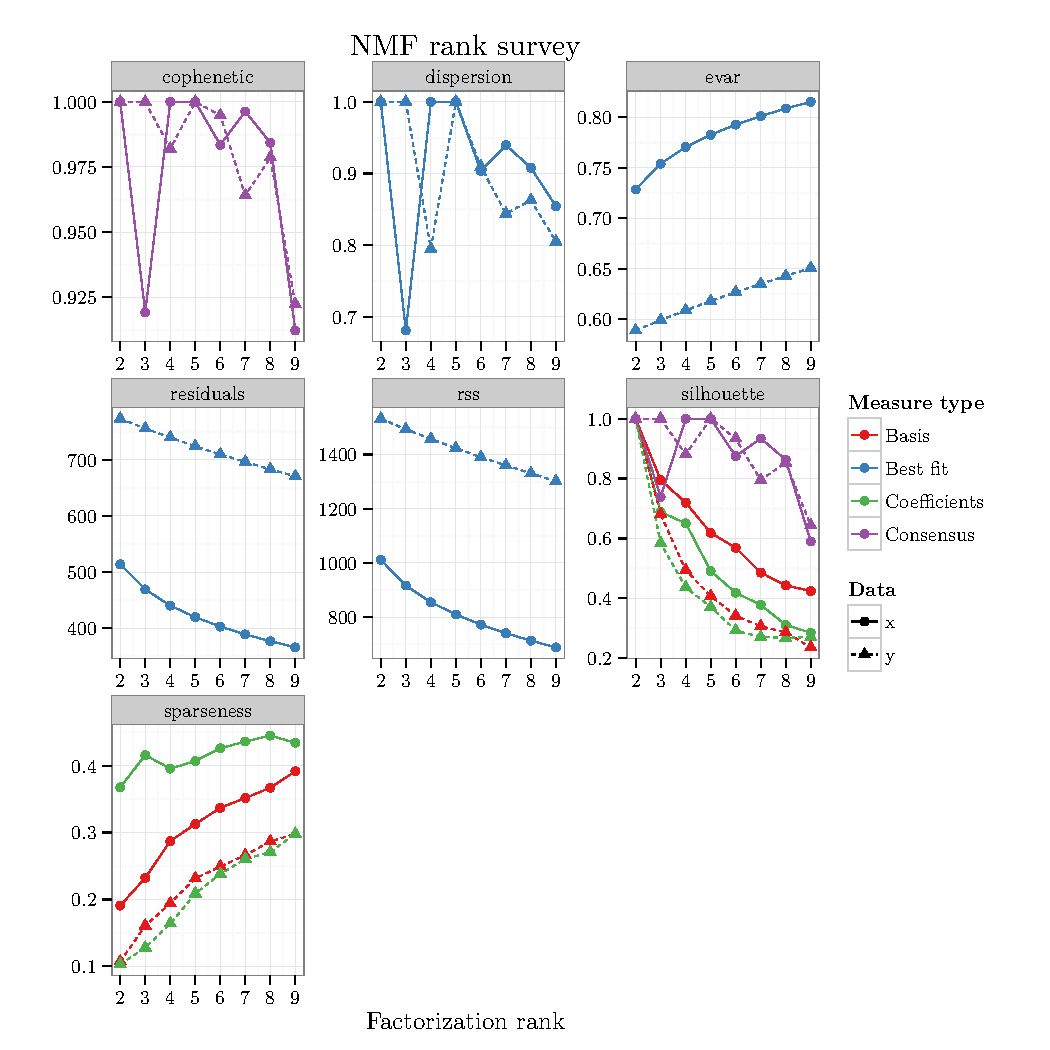
\includegraphics[width=\maxwidth]{figure/nmf-rank-plots-1} 

}


\begin{kframe}\begin{alltt}
\hlkwd{plot}\hlstd{(nmf.rankrange[}\hlopt{-}\hlnum{1}\hlstd{],} \hlopt{-}\hlstd{temp.orig_resids.delta,} \hlkwc{type} \hlstd{=} \hlstr{"o"}\hlstd{,} \hlkwc{col} \hlstd{=} \hlstr{"black"}\hlstd{,}
    \hlkwc{pch} \hlstd{=} \hlnum{21}\hlstd{,} \hlkwc{ylim} \hlstd{=} \hlkwd{range}\hlstd{(}\hlopt{-}\hlkwd{c}\hlstd{(temp.orig_resids.delta, temp.perm_resids.delta.mean)),}
    \hlkwc{xlab} \hlstd{=} \hlstr{"Factorization Rank Added"}\hlstd{,} \hlkwc{ylab} \hlstd{=} \hlstr{"Improvement in Total Residual Error"}\hlstd{)}
\hlkwd{lines}\hlstd{(nmf.rankrange[}\hlopt{-}\hlnum{1}\hlstd{],} \hlopt{-}\hlstd{temp.perm_resids.delta.mean,} \hlkwc{col} \hlstd{=} \hlstr{"red"}\hlstd{,} \hlkwc{type} \hlstd{=} \hlstr{"o"}\hlstd{,}
    \hlkwc{pch} \hlstd{=} \hlnum{21}\hlstd{,} \hlkwc{lwd} \hlstd{=} \hlnum{1}\hlstd{)}
\hlkwa{for} \hlstd{(i} \hlkwa{in} \hlnum{1}\hlopt{:}\hlkwd{ncol}\hlstd{(temp.perm_resids)) \{}
    \hlkwd{lines}\hlstd{(nmf.rankrange[}\hlopt{-}\hlnum{1}\hlstd{],} \hlopt{-}\hlstd{temp.perm_resids.delta[, i],} \hlkwc{type} \hlstd{=} \hlstr{"o"}\hlstd{,} \hlkwc{col} \hlstd{=} \hlkwd{rgb}\hlstd{(}\hlnum{1}\hlstd{,}
        \hlnum{0}\hlstd{,} \hlnum{0}\hlstd{,} \hlnum{0.25}\hlstd{))}
\hlstd{\}}
\hlkwd{lines}\hlstd{(nmf.rankrange[}\hlopt{-}\hlnum{1}\hlstd{],} \hlopt{-}\hlstd{temp.perm_resids.delta.threshold,} \hlkwc{col} \hlstd{=} \hlstr{"red"}\hlstd{,} \hlkwc{lty} \hlstd{=} \hlstr{"dotted"}\hlstd{)}
\hlkwa{if} \hlstd{(nmf.rank.wasauto} \hlopt{==} \hlnum{TRUE}\hlstd{) \{}
    \hlstd{temp.col} \hlkwb{=} \hlstr{"green"}
\hlstd{\}} \hlkwa{else} \hlstd{\{}
    \hlstd{temp.col} \hlkwb{=} \hlstr{"blue"}
\hlstd{\}}
\hlkwd{abline}\hlstd{(}\hlkwc{v} \hlstd{= nmf.rank,} \hlkwc{col} \hlstd{= temp.col,} \hlkwc{lwd} \hlstd{=} \hlnum{2}\hlstd{)}
\hlkwd{legend}\hlstd{(}\hlstr{"topright"}\hlstd{,} \hlkwc{legend} \hlstd{=} \hlkwd{c}\hlstd{(}\hlstr{"Original data"}\hlstd{,} \hlstr{"Permuted data"}\hlstd{,} \hlkwd{sprintf}\hlstd{(}\hlstr{"Selected rank (%s)"}\hlstd{,}
    \hlkwd{ifelse}\hlstd{(nmf.rank.wasauto} \hlopt{==} \hlnum{TRUE}\hlstd{,} \hlstr{"auto"}\hlstd{,} \hlstr{"fixed"}\hlstd{))),} \hlkwc{col} \hlstd{=} \hlkwd{c}\hlstd{(}\hlstr{"black"}\hlstd{,} \hlstr{"red"}\hlstd{,}
    \hlstd{temp.col),} \hlkwc{lty} \hlstd{=} \hlstr{"solid"}\hlstd{,} \hlkwc{pch} \hlstd{=} \hlnum{21}\hlstd{,} \hlkwc{inset} \hlstd{=} \hlnum{0.05}\hlstd{)}
\end{alltt}
\end{kframe}

{\centering 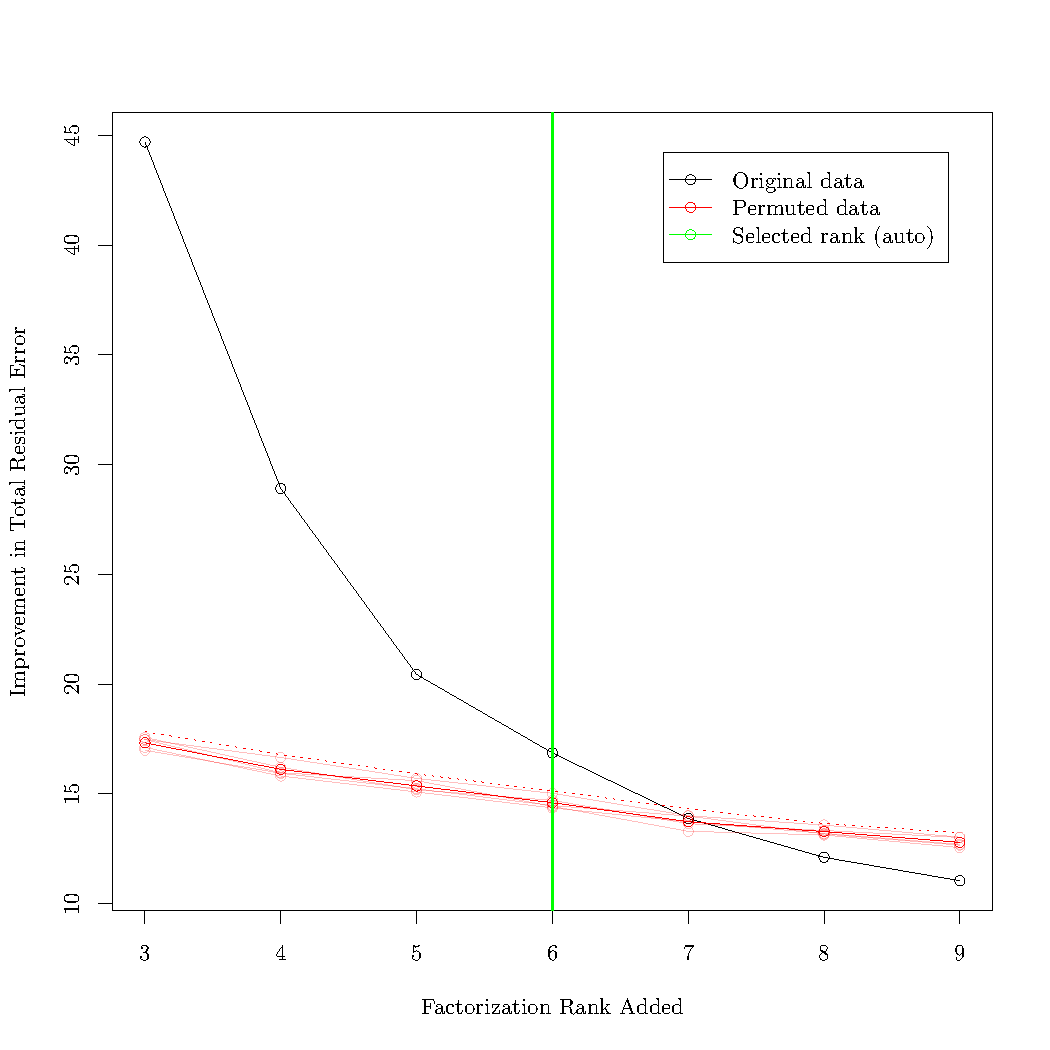
\includegraphics[width=\maxwidth]{figure/nmf-rank-plots-2} 

}



\end{knitrout}

\subsection{Fit}
\begin{knitrout}
\definecolor{shadecolor}{rgb}{0.969, 0.969, 0.969}\color{fgcolor}\begin{kframe}
\begin{alltt}
\hlkwd{consensusmap}\hlstd{(nmf.final)}
\end{alltt}
\end{kframe}

{\centering 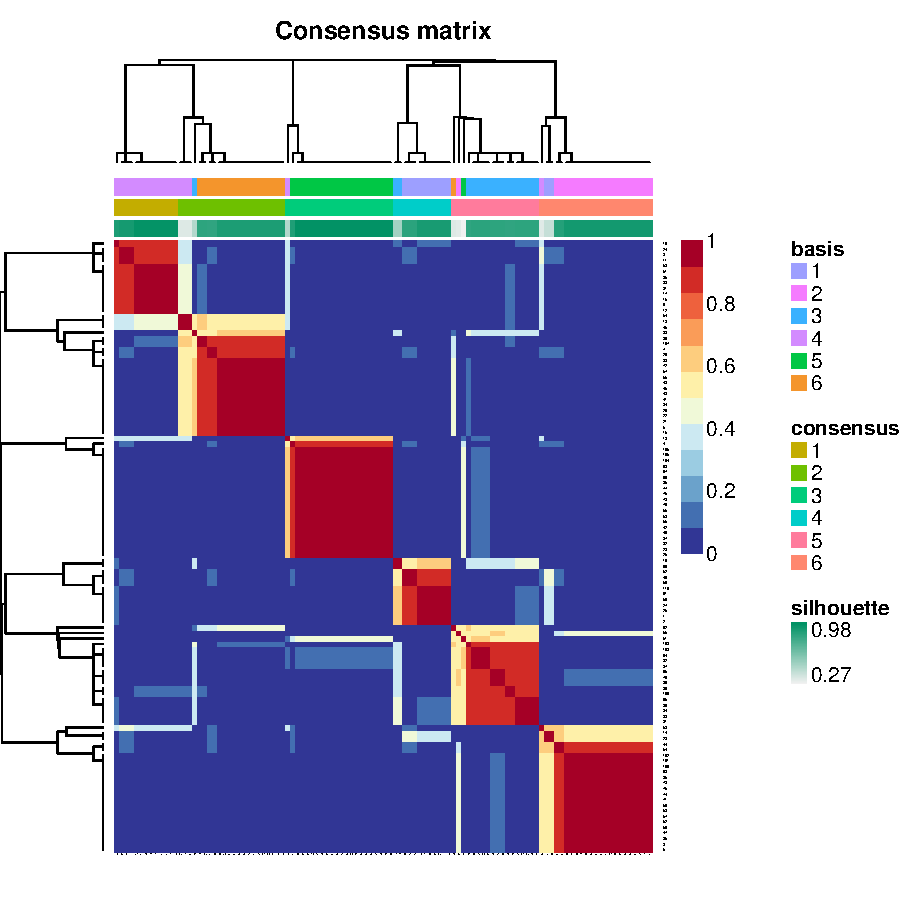
\includegraphics[width=\maxwidth]{figure/nmf-plots-1} 

}


\begin{kframe}\begin{alltt}
\hlkwd{basismap}\hlstd{(nmf.final)}
\end{alltt}
\end{kframe}

{\centering 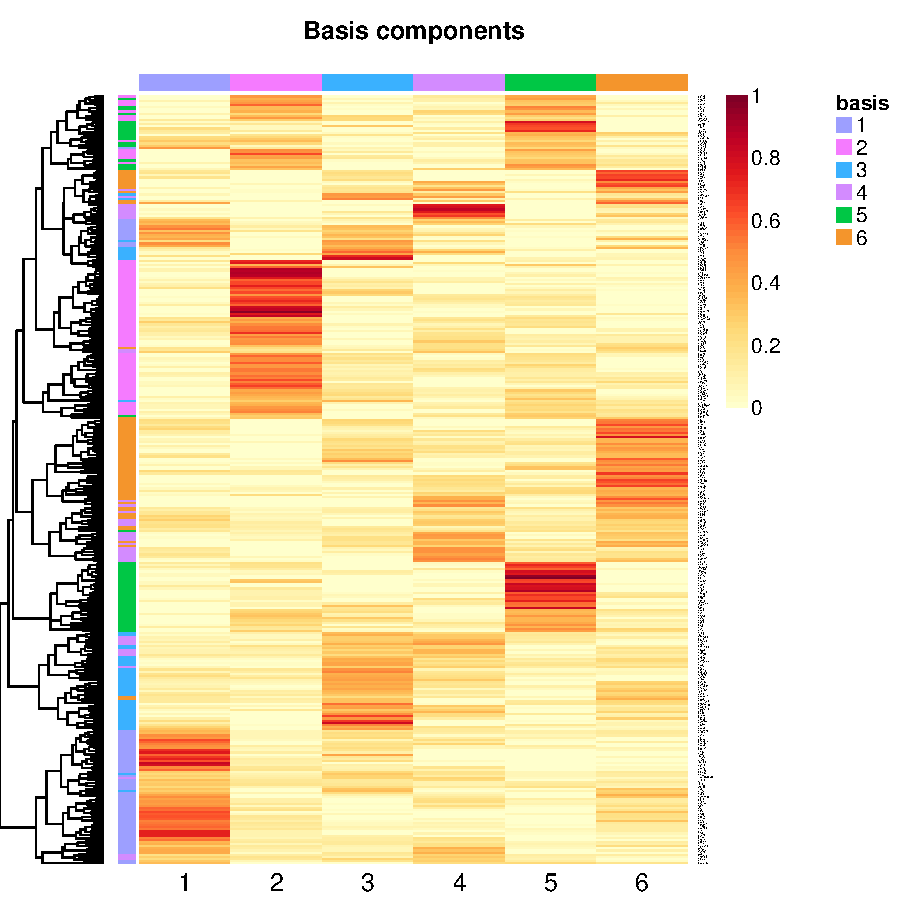
\includegraphics[width=\maxwidth]{figure/nmf-plots-2} 

}


\begin{kframe}\begin{alltt}
\hlkwd{coefmap}\hlstd{(nmf.final)}
\end{alltt}
\end{kframe}

{\centering 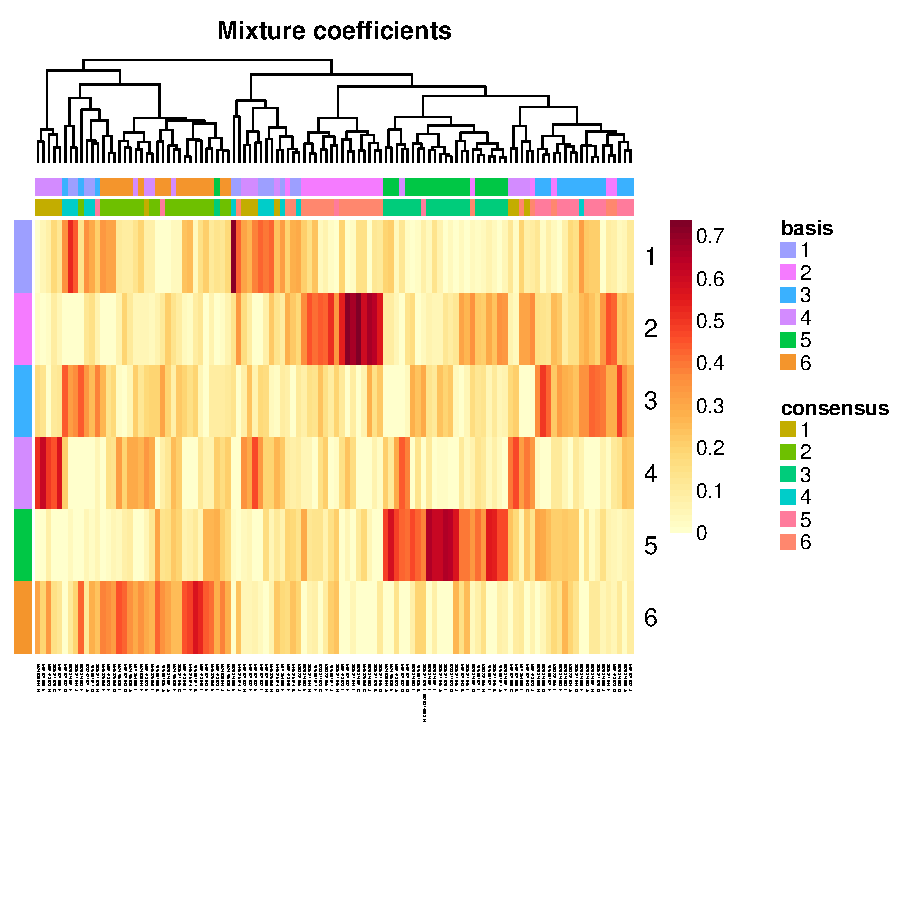
\includegraphics[width=\maxwidth]{figure/nmf-plots-3} 

}



\end{knitrout}


%%%%%%%%%%%%%%%%%%%%%%%%%%%%%%%%%%%%%%%%%%%%%%%%%%%%%%%%%%%%%%%%%%%%%%
% SIGNATURE ESTIMATION
%%%%%%%%%%%%%%%%%%%%%%%%%%%%%%%%%%%%%%%%%%%%%%%%%%%%%%%%%%%%%%%%%%%%%%
\begin{knitrout}
\definecolor{shadecolor}{rgb}{0.969, 0.969, 0.969}\color{fgcolor}\begin{kframe}
\begin{alltt}
\hlstd{coefs.diag_dsd} \hlkwb{=} \hlkwd{apply}\hlstd{(xlin.diag_dsd.sel,} \hlnum{2}\hlstd{,} \hlkwa{function}\hlstd{(}\hlkwc{xcol}\hlstd{)} \hlkwd{nnls}\hlstd{(}\hlkwd{basis}\hlstd{(nmf.final),}
    \hlstd{xcol)}\hlopt{$}\hlstd{x)}
\hlstd{coefs.diag_rec} \hlkwb{=} \hlkwd{apply}\hlstd{(xlin.diag_rec.sel,} \hlnum{2}\hlstd{,} \hlkwa{function}\hlstd{(}\hlkwc{xcol}\hlstd{)} \hlkwd{nnls}\hlstd{(}\hlkwd{basis}\hlstd{(nmf.final),}
    \hlstd{xcol)}\hlopt{$}\hlstd{x)}
\hlstd{coefs.recr_dsd} \hlkwb{=} \hlkwd{apply}\hlstd{(xlin.recr_dsd.sel,} \hlnum{2}\hlstd{,} \hlkwa{function}\hlstd{(}\hlkwc{xcol}\hlstd{)} \hlkwd{nnls}\hlstd{(}\hlkwd{basis}\hlstd{(nmf.final),}
    \hlstd{xcol)}\hlopt{$}\hlstd{x)}
\hlstd{coefs.pdac_au} \hlkwb{=} \hlkwd{apply}\hlstd{(xlin.pdac_au.sel,} \hlnum{2}\hlstd{,} \hlkwa{function}\hlstd{(}\hlkwc{xcol}\hlstd{)} \hlkwd{nnls}\hlstd{(}\hlkwd{basis}\hlstd{(nmf.final),}
    \hlstd{xcol)}\hlopt{$}\hlstd{x)}
\end{alltt}
\end{kframe}
\end{knitrout}





\begin{knitrout}
\definecolor{shadecolor}{rgb}{0.969, 0.969, 0.969}\color{fgcolor}\begin{kframe}
\begin{alltt}
\hlstd{temp.pred.pairs} \hlkwb{=} \hlkwd{t}\hlstd{(}\hlkwd{rbind}\hlstd{(coefs.pdac_au, metapcna.scores[}\hlkwd{colnames}\hlstd{(coefs.pdac_au)]))}
\hlkwd{colnames}\hlstd{(temp.pred.pairs)} \hlkwb{=} \hlkwd{paste}\hlstd{(}\hlstr{"mg"}\hlstd{,} \hlnum{1}\hlopt{:}\hlkwd{ncol}\hlstd{(temp.pred.pairs),} \hlkwc{sep} \hlstd{=} \hlstr{"."}\hlstd{)}
\hlkwd{colnames}\hlstd{(temp.pred.pairs)[}\hlkwd{ncol}\hlstd{(temp.pred.pairs)]} \hlkwb{=} \hlstr{"PCNA"}
\hlstd{temp.pred.pairs} \hlkwb{=} \hlkwd{cbind}\hlstd{(temp.pred.pairs,} \hlkwc{qpure} \hlstd{= samps.pdac_au}\hlopt{$}\hlstd{purity_qpure,}
    \hlkwc{pkyrs} \hlstd{= cpvs.pdac_au}\hlopt{$}\hlstd{History.Smoking.PackYears)}
\hlkwd{pairs}\hlstd{(temp.pred.pairs,} \hlkwc{pch} \hlstd{=} \hlnum{16}\hlstd{,} \hlkwc{cex} \hlstd{=} \hlnum{1}\hlstd{,} \hlkwc{col} \hlstd{=} \hlkwd{ifelse}\hlstd{(}\hlkwd{rownames}\hlstd{(temp.pred.pairs)} \hlopt
    \hlkwd{colnames}\hlstd{(xlin.diag_dsd.sel),} \hlkwd{rgb}\hlstd{(}\hlnum{0}\hlstd{,} \hlnum{0}\hlstd{,} \hlnum{0}\hlstd{,} \hlnum{0.5}\hlstd{),} \hlkwd{rgb}\hlstd{(}\hlnum{1}\hlstd{,} \hlnum{0}\hlstd{,} \hlnum{1}\hlstd{,} \hlnum{0.5}\hlstd{)))}
\end{alltt}
\end{kframe}

{\centering 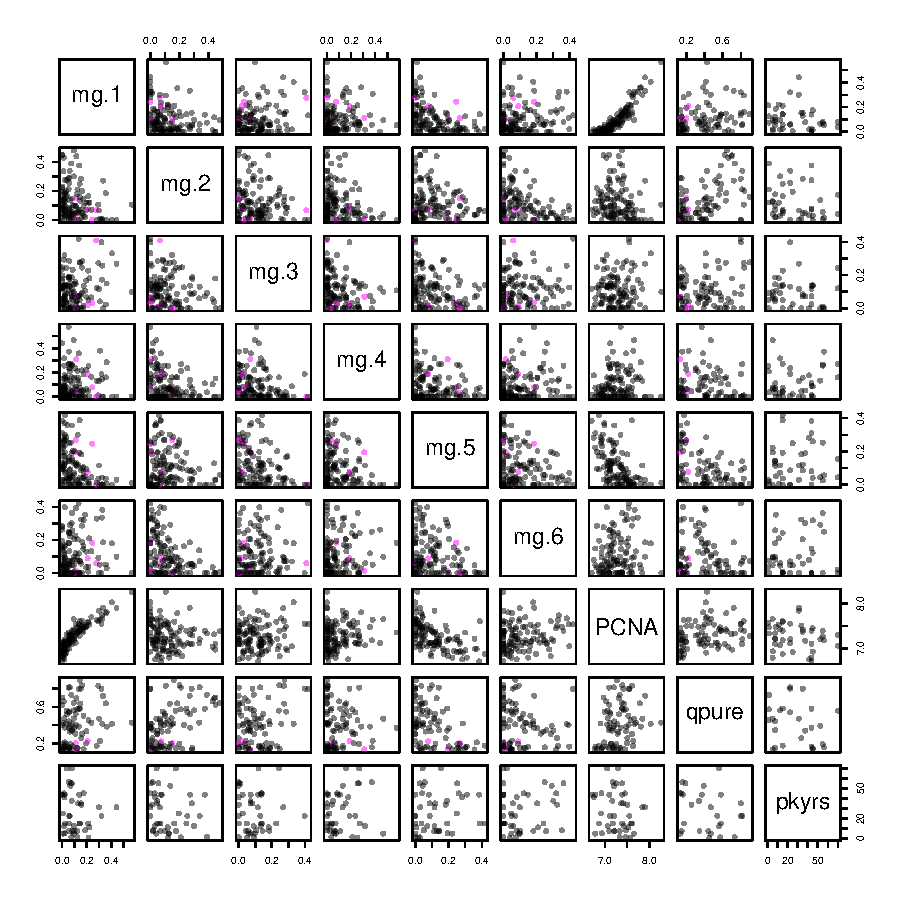
\includegraphics[width=\maxwidth]{figure/metagene-pairs-1} 

}


\begin{kframe}\begin{alltt}
\hlstd{temp.pred.pairs.rescaled} \hlkwb{=} \hlkwd{t}\hlstd{((}\hlkwd{t}\hlstd{(temp.pred.pairs)} \hlopt{-} \hlkwd{apply}\hlstd{(temp.pred.pairs,} \hlnum{2}\hlstd{,}
    \hlstd{min,} \hlkwc{na.rm} \hlstd{=} \hlnum{TRUE}\hlstd{))}\hlopt{/}\hlstd{(}\hlkwd{apply}\hlstd{(temp.pred.pairs,} \hlnum{2}\hlstd{,} \hlkwa{function}\hlstd{(}\hlkwc{x}\hlstd{)} \hlkwd{diff}\hlstd{(}\hlkwd{range}\hlstd{(x,}
    \hlkwc{na.rm} \hlstd{=} \hlnum{TRUE}\hlstd{)))))}
\hlkwd{heatmap.2}\hlstd{(temp.pred.pairs.rescaled,} \hlkwc{trace} \hlstd{=} \hlstr{"none"}\hlstd{,} \hlkwc{scale} \hlstd{=} \hlstr{"none"}\hlstd{,} \hlkwc{col} \hlstd{=} \hlkwd{brewer.pal}\hlstd{(}\hlnum{9}\hlstd{,}
    \hlstr{"GnBu"}\hlstd{))}
\end{alltt}
\end{kframe}

{\centering 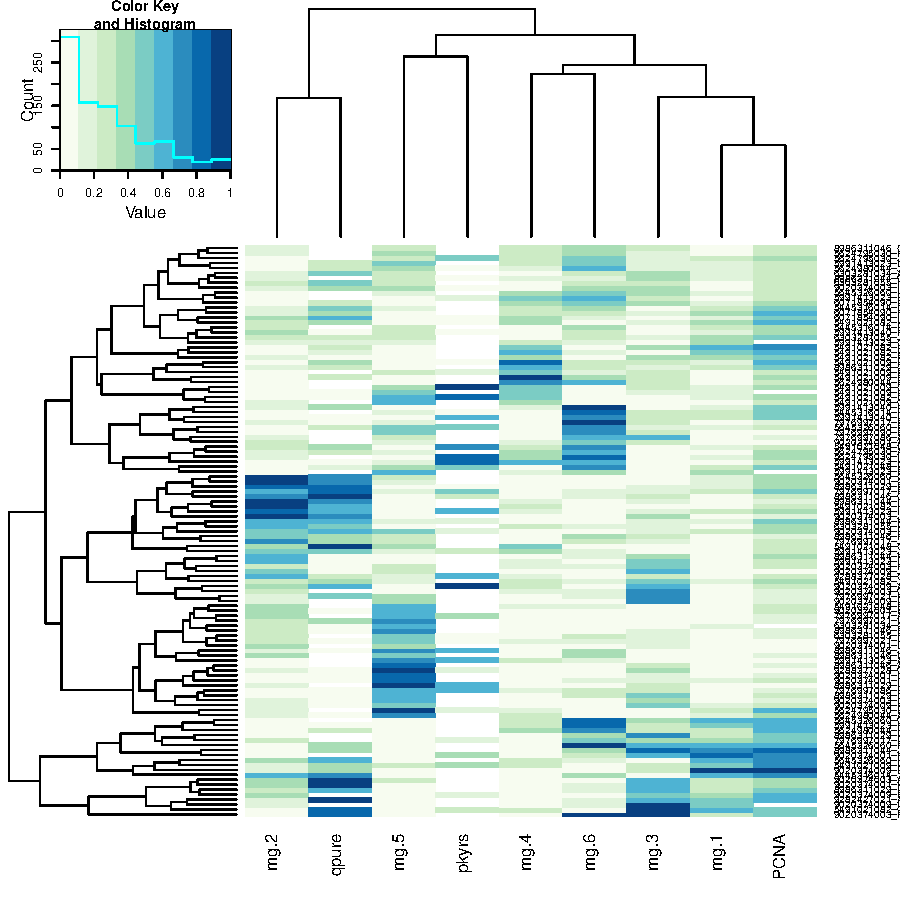
\includegraphics[width=\maxwidth]{figure/metagene-pairs-2} 

}


\begin{kframe}\begin{alltt}
\hlkwd{heatmap.2}\hlstd{(temp.pred.pairs.rescaled[}\hlkwd{apply}\hlstd{(}\hlopt{!}\hlkwd{is.na}\hlstd{(temp.pred.pairs.rescaled),} \hlnum{1}\hlstd{,}
    \hlstd{all), ],} \hlkwc{trace} \hlstd{=} \hlstr{"none"}\hlstd{,} \hlkwc{scale} \hlstd{=} \hlstr{"none"}\hlstd{,} \hlkwc{col} \hlstd{=} \hlkwd{brewer.pal}\hlstd{(}\hlnum{9}\hlstd{,} \hlstr{"GnBu"}\hlstd{))}
\end{alltt}
\end{kframe}

{\centering 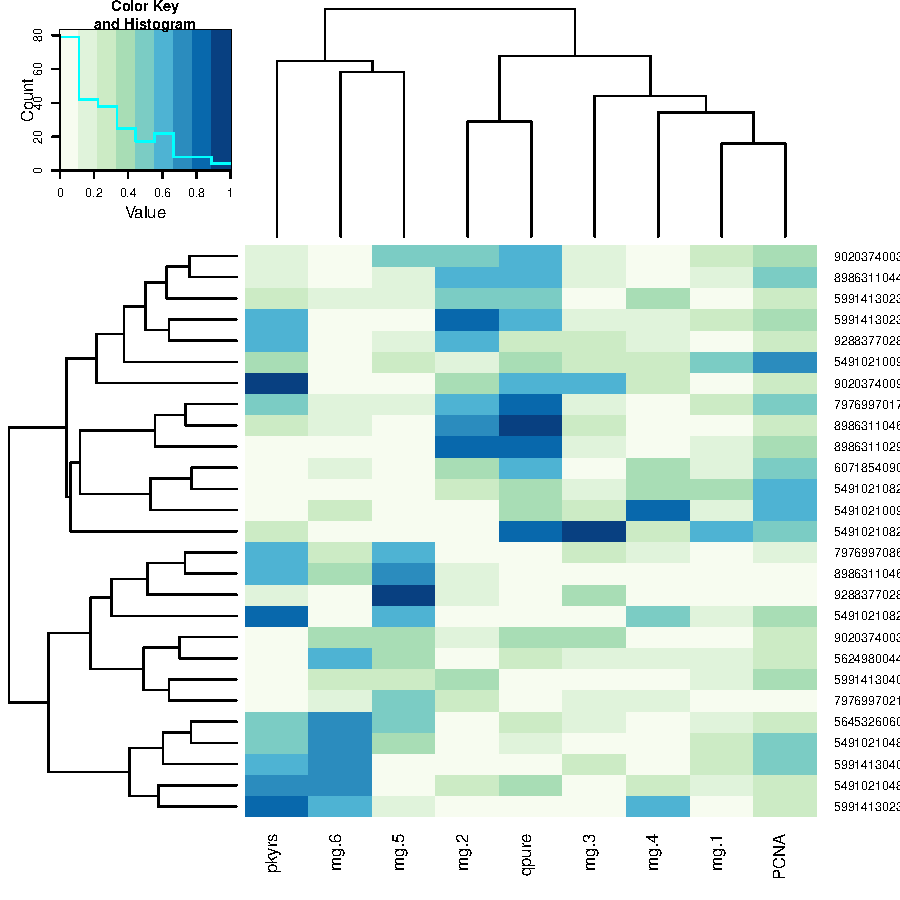
\includegraphics[width=\maxwidth]{figure/metagene-pairs-3} 

}


\begin{kframe}\begin{alltt}
\hlstd{temp.pred.pairs.rescaled2} \hlkwb{=} \hlstd{temp.pred.pairs.rescaled[,} \hlkwd{colnames}\hlstd{(temp.pred.pairs.rescaled)} \hlopt{!=}
    \hlstr{"pkyrs"}\hlstd{]}
\hlkwd{heatmap.2}\hlstd{(temp.pred.pairs.rescaled2,} \hlkwc{trace} \hlstd{=} \hlstr{"none"}\hlstd{,} \hlkwc{scale} \hlstd{=} \hlstr{"none"}\hlstd{,} \hlkwc{col} \hlstd{=} \hlkwd{brewer.pal}\hlstd{(}\hlnum{9}\hlstd{,}
    \hlstr{"GnBu"}\hlstd{))}
\end{alltt}
\end{kframe}

{\centering 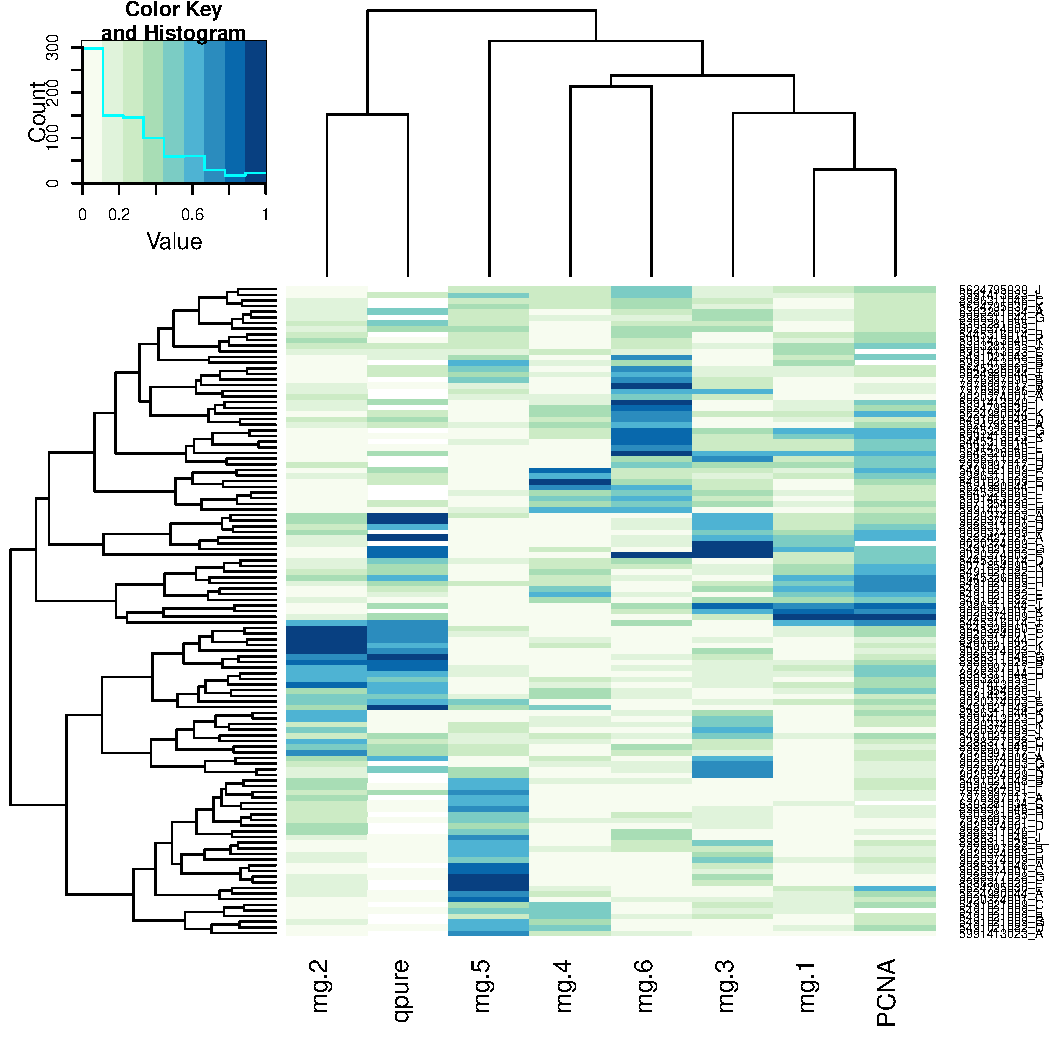
\includegraphics[width=\maxwidth]{figure/metagene-pairs-4} 

}


\begin{kframe}\begin{alltt}
\hlkwd{heatmap.2}\hlstd{(temp.pred.pairs.rescaled2[}\hlkwd{apply}\hlstd{(}\hlopt{!}\hlkwd{is.na}\hlstd{(temp.pred.pairs.rescaled2),}
    \hlnum{1}\hlstd{, all), ],} \hlkwc{trace} \hlstd{=} \hlstr{"none"}\hlstd{,} \hlkwc{scale} \hlstd{=} \hlstr{"none"}\hlstd{,} \hlkwc{col} \hlstd{=} \hlkwd{brewer.pal}\hlstd{(}\hlnum{9}\hlstd{,} \hlstr{"GnBu"}\hlstd{))}
\end{alltt}
\end{kframe}

{\centering 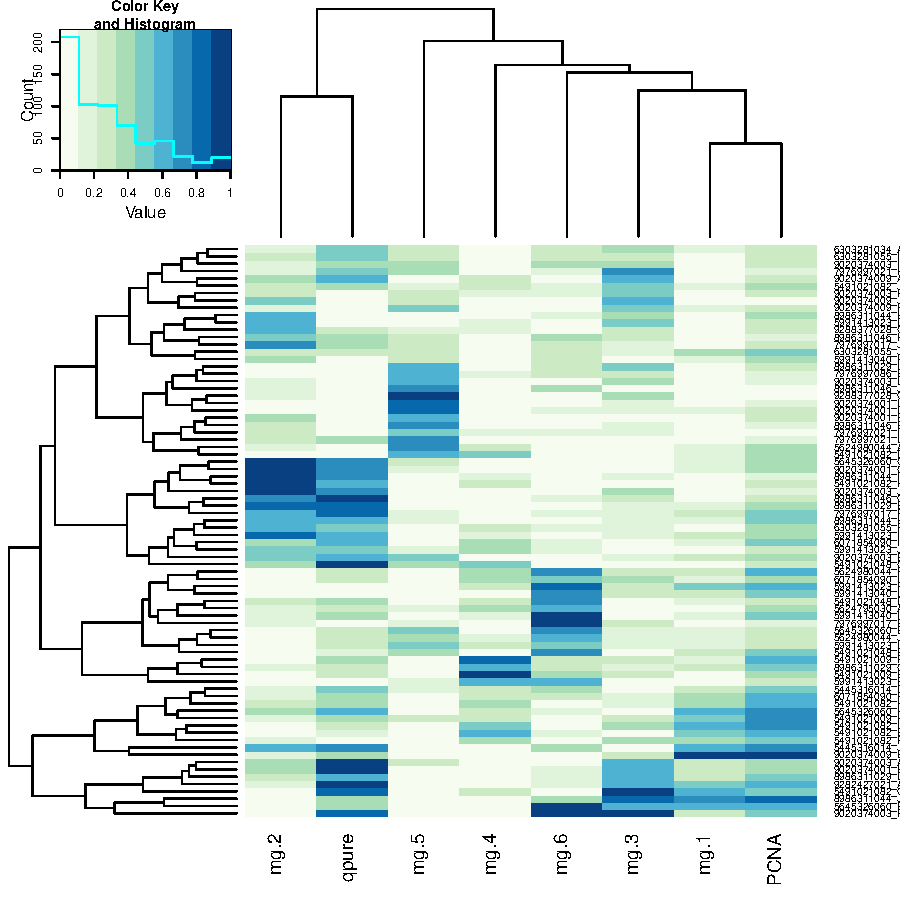
\includegraphics[width=\maxwidth]{figure/metagene-pairs-5} 

}


\begin{kframe}\begin{alltt}
\hlstd{temp.cors} \hlkwb{=} \hlkwd{apply}\hlstd{(temp.pred.pairs[,} \hlkwd{colnames}\hlstd{(temp.pred.pairs)} \hlopt{!=} \hlstr{"pkyrs"}\hlstd{],} \hlnum{2}\hlstd{,}
    \hlkwa{function}\hlstd{(}\hlkwc{x}\hlstd{)} \hlkwd{apply}\hlstd{(temp.pred.pairs[,} \hlkwd{colnames}\hlstd{(temp.pred.pairs)} \hlopt{!=} \hlstr{"pkyrs"}\hlstd{],}
        \hlnum{2}\hlstd{,} \hlkwa{function}\hlstd{(}\hlkwc{y}\hlstd{) \{}
            \hlstd{sel} \hlkwb{=} \hlopt{!}\hlstd{(}\hlkwd{is.na}\hlstd{(x)} \hlopt{|} \hlkwd{is.na}\hlstd{(y))}
            \hlkwd{cor}\hlstd{(x[sel], y[sel],} \hlkwc{method} \hlstd{=} \hlstr{"kendall"}\hlstd{)}
        \hlstd{\}))}
\hlcom{# diag(temp.cors) = NA}
\hlkwd{heatmap.2}\hlstd{(temp.cors,} \hlkwc{trace} \hlstd{=} \hlstr{"none"}\hlstd{,} \hlkwc{Rowv} \hlstd{=} \hlnum{FALSE}\hlstd{,} \hlkwc{Colv} \hlstd{=} \hlnum{FALSE}\hlstd{,} \hlkwc{col} \hlstd{=} \hlkwd{brewer.pal}\hlstd{(}\hlnum{11}\hlstd{,}
    \hlstr{"PiYG"}\hlstd{),} \hlkwc{dendrogram} \hlstd{=} \hlstr{"none"}\hlstd{,} \hlkwc{scale} \hlstd{=} \hlstr{"none"}\hlstd{)}
\end{alltt}
\end{kframe}

{\centering 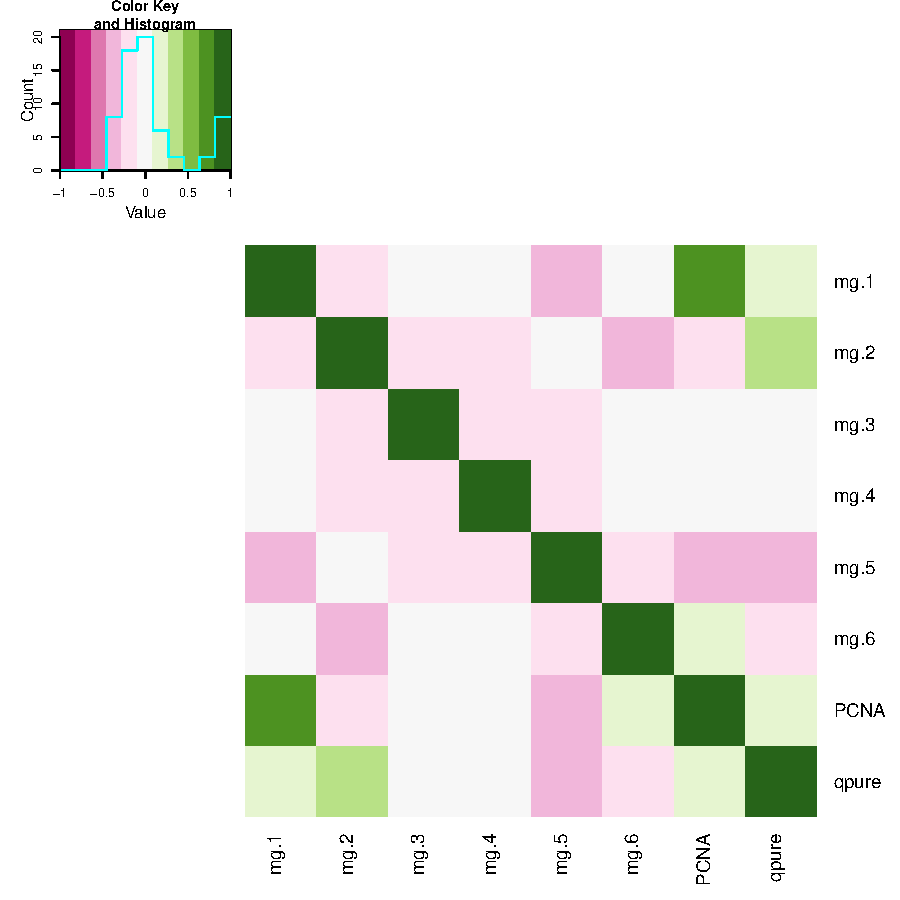
\includegraphics[width=\maxwidth]{figure/metagene-pairs-6} 

}



\end{knitrout}


%%%%%%%%%%%%%%%%%%%%%%%%%%%%%%%%%%%%%%%%%%%%%%%%%%%%%%%%%%%%%%%%%%%%%%
% SIGNATURE PROGNOSTIC PERFORMANCE: TRAINING SET, ALONE
%%%%%%%%%%%%%%%%%%%%%%%%%%%%%%%%%%%%%%%%%%%%%%%%%%%%%%%%%%%%%%%%%%%%%%
\subsection{LASSO on training set}
\begin{knitrout}
\definecolor{shadecolor}{rgb}{0.969, 0.969, 0.969}\color{fgcolor}\begin{kframe}
\begin{alltt}
\hlstd{glmnet.fit.cv.diag_dsd} \hlkwb{=} \hlkwd{cv.glmnet}\hlstd{(}\hlkwd{t}\hlstd{(coefs.diag_dsd), y.diag_dsd,} \hlkwc{family} \hlstd{=} \hlstr{"cox"}\hlstd{,}
    \hlkwc{nfolds} \hlstd{=} \hlnum{10}\hlstd{)}
\hlstd{glmnet.fit.cv.diag_rec} \hlkwb{=} \hlkwd{cv.glmnet}\hlstd{(}\hlkwd{t}\hlstd{(coefs.diag_rec), y.diag_rec,} \hlkwc{family} \hlstd{=} \hlstr{"cox"}\hlstd{,}
    \hlkwc{nfolds} \hlstd{=} \hlnum{10}\hlstd{)}
\hlstd{glmnet.fit.cv.recr_dsd} \hlkwb{=} \hlkwd{cv.glmnet}\hlstd{(}\hlkwd{t}\hlstd{(coefs.recr_dsd), y.recr_dsd,} \hlkwc{family} \hlstd{=} \hlstr{"cox"}\hlstd{,}
    \hlkwc{nfolds} \hlstd{=} \hlnum{10}\hlstd{)}
\end{alltt}
\end{kframe}
\end{knitrout}

\begin{knitrout}
\definecolor{shadecolor}{rgb}{0.969, 0.969, 0.969}\color{fgcolor}\begin{kframe}
\begin{alltt}
\hlkwd{plot}\hlstd{(glmnet.fit.cv.diag_dsd)}
\end{alltt}
\end{kframe}

{\centering 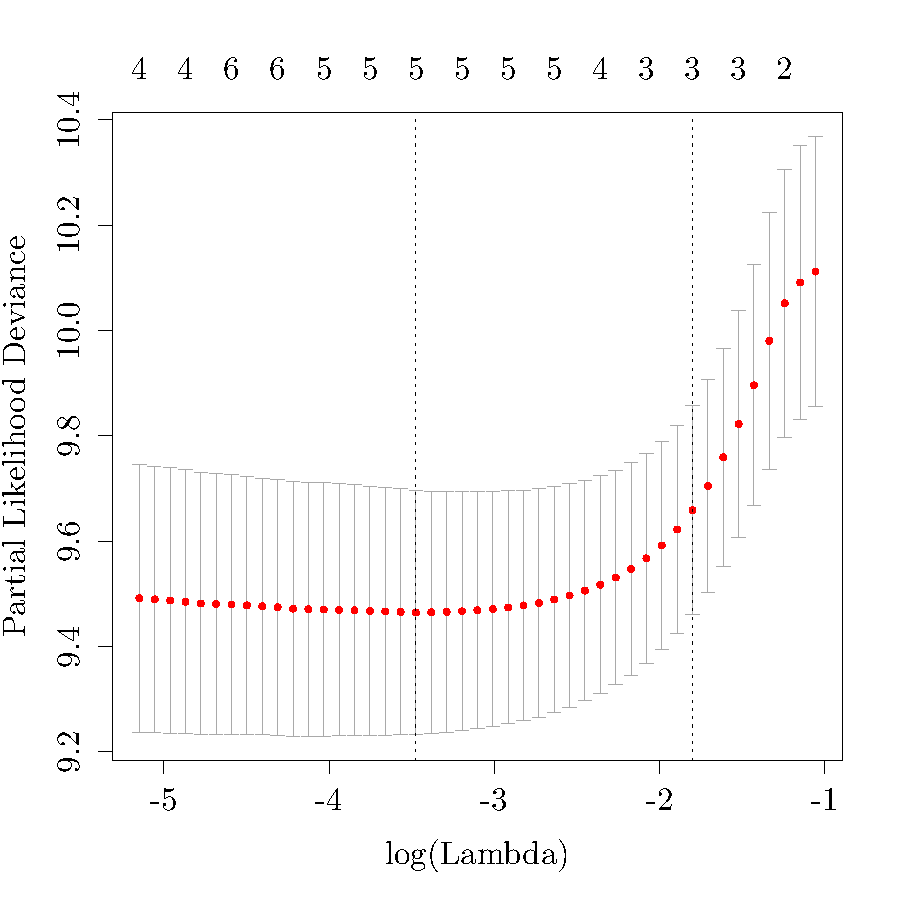
\includegraphics[width=\maxwidth]{figure/nmf-metagene-glmnet-plots-1} 

}


\begin{kframe}\begin{alltt}
\hlkwd{plot}\hlstd{(glmnet.fit.cv.diag_dsd}\hlopt{$}\hlstd{glmnet.fit,} \hlkwc{label} \hlstd{=} \hlnum{TRUE}\hlstd{)}
\hlkwd{abline}\hlstd{(}\hlkwc{v} \hlstd{=} \hlkwd{sum}\hlstd{(}\hlkwd{abs}\hlstd{(}\hlkwd{coef}\hlstd{(glmnet.fit.cv.diag_dsd}\hlopt{$}\hlstd{glmnet.fit,} \hlkwc{s} \hlstd{= glmnet.fit.cv.diag_dsd}\hlopt{$}\hlstd{lambda.1se))))}
\end{alltt}
\end{kframe}

{\centering 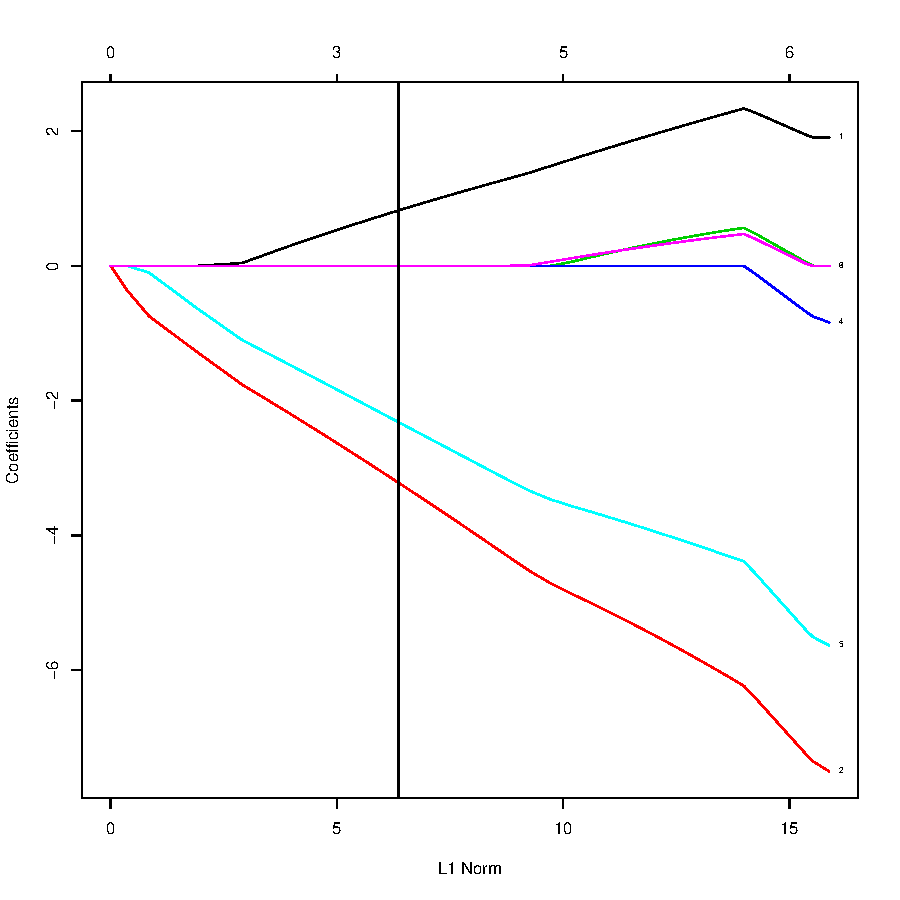
\includegraphics[width=\maxwidth]{figure/nmf-metagene-glmnet-plots-2} 

}


\begin{kframe}\begin{alltt}
\hlcom{# abline(v = sum(abs(coef(glmnet.fit.cv.diag_dsd$glmnet.fit, s =}
\hlcom{# glmnet.fit.cv.diag_dsd$lambda.min))))}
\hlkwd{coef}\hlstd{(glmnet.fit.cv.diag_dsd}\hlopt{$}\hlstd{glmnet.fit,} \hlkwc{s} \hlstd{= glmnet.fit.cv.diag_dsd}\hlopt{$}\hlstd{lambda.1se)}
\end{alltt}
\begin{verbatim}
## 6 x 1 sparse Matrix of class "dgCMatrix"
##          1
## V1  0.8238
## V2 -3.2195
## V3  .     
## V4  .     
## V5 -2.3208
## V6  .
\end{verbatim}
\begin{alltt}
\hlkwd{plot}\hlstd{(glmnet.fit.cv.diag_rec)}
\end{alltt}
\end{kframe}

{\centering 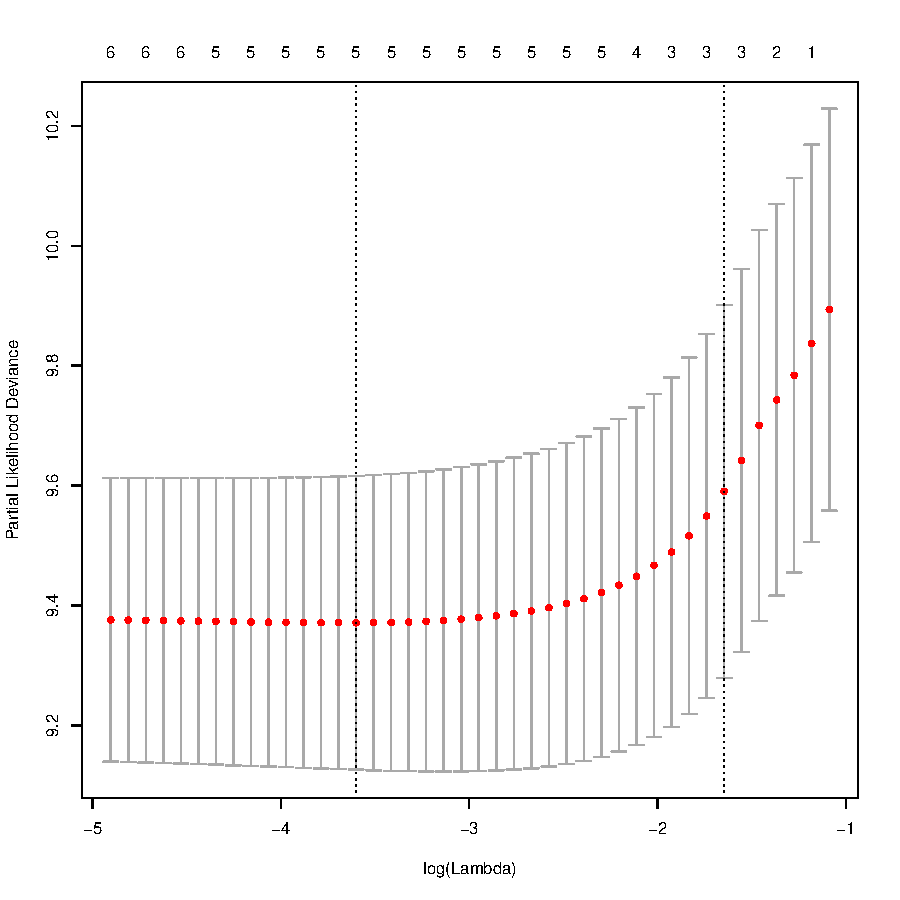
\includegraphics[width=\maxwidth]{figure/nmf-metagene-glmnet-plots-3} 

}


\begin{kframe}\begin{alltt}
\hlkwd{plot}\hlstd{(glmnet.fit.cv.diag_rec}\hlopt{$}\hlstd{glmnet.fit,} \hlkwc{label} \hlstd{=} \hlnum{TRUE}\hlstd{)}
\hlkwd{abline}\hlstd{(}\hlkwc{v} \hlstd{=} \hlkwd{sum}\hlstd{(}\hlkwd{abs}\hlstd{(}\hlkwd{coef}\hlstd{(glmnet.fit.cv.diag_rec}\hlopt{$}\hlstd{glmnet.fit,} \hlkwc{s} \hlstd{= glmnet.fit.cv.diag_rec}\hlopt{$}\hlstd{lambda.1se))))}
\end{alltt}
\end{kframe}

{\centering 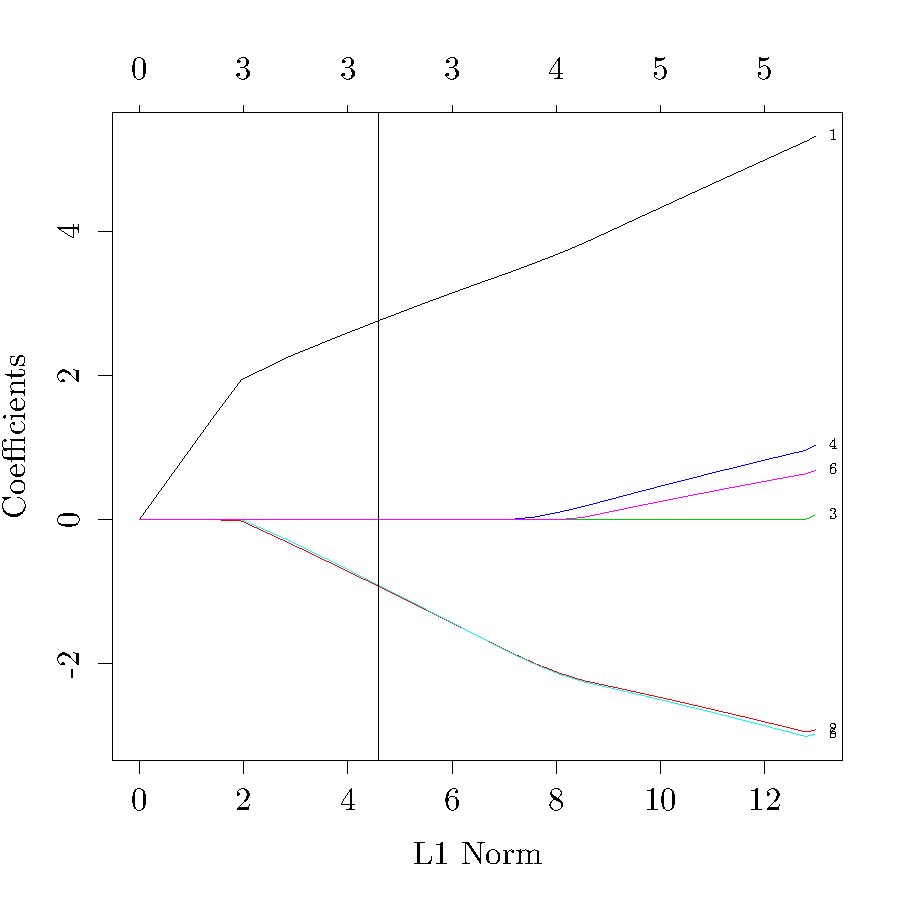
\includegraphics[width=\maxwidth]{figure/nmf-metagene-glmnet-plots-4} 

}


\begin{kframe}\begin{alltt}
\hlcom{# abline(v = sum(abs(coef(glmnet.fit.cv.diag_rec$glmnet.fit, s =}
\hlcom{# glmnet.fit.cv.diag_rec$lambda.min))))}
\hlkwd{coef}\hlstd{(glmnet.fit.cv.diag_rec}\hlopt{$}\hlstd{glmnet.fit,} \hlkwc{s} \hlstd{= glmnet.fit.cv.diag_rec}\hlopt{$}\hlstd{lambda.1se)}
\end{alltt}
\begin{verbatim}
## 6 x 1 sparse Matrix of class "dgCMatrix"
##          1
## V1  2.2667
## V2 -0.3332
## V3  .     
## V4  .     
## V5 -0.2974
## V6  .
\end{verbatim}
\begin{alltt}
\hlkwd{plot}\hlstd{(glmnet.fit.cv.recr_dsd)}
\end{alltt}
\end{kframe}

{\centering 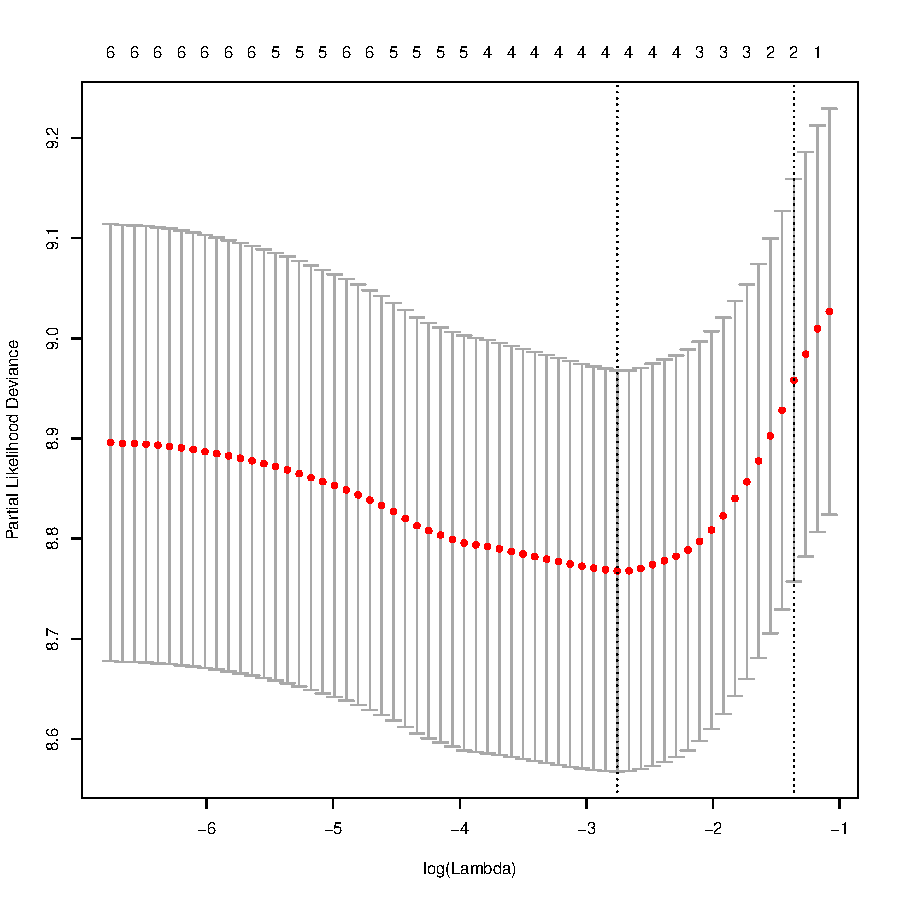
\includegraphics[width=\maxwidth]{figure/nmf-metagene-glmnet-plots-5} 

}


\begin{kframe}\begin{alltt}
\hlkwd{plot}\hlstd{(glmnet.fit.cv.recr_dsd}\hlopt{$}\hlstd{glmnet.fit,} \hlkwc{label} \hlstd{=} \hlnum{TRUE}\hlstd{)}
\hlkwd{abline}\hlstd{(}\hlkwc{v} \hlstd{=} \hlkwd{sum}\hlstd{(}\hlkwd{abs}\hlstd{(}\hlkwd{coef}\hlstd{(glmnet.fit.cv.recr_dsd}\hlopt{$}\hlstd{glmnet.fit,} \hlkwc{s} \hlstd{= glmnet.fit.cv.recr_dsd}\hlopt{$}\hlstd{lambda.1se))))}
\end{alltt}
\end{kframe}

{\centering 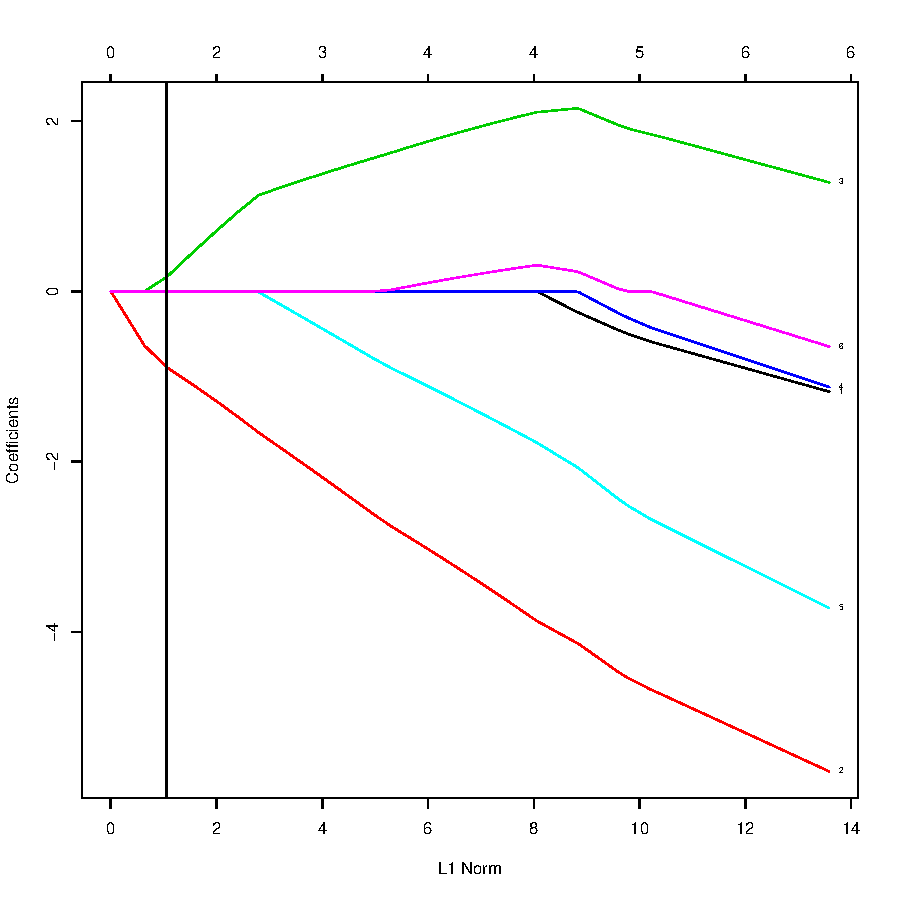
\includegraphics[width=\maxwidth]{figure/nmf-metagene-glmnet-plots-6} 

}


\begin{kframe}\begin{alltt}
\hlcom{# abline(v = sum(abs(coef(glmnet.fit.cv.recr_dsd$glmnet.fit, s =}
\hlcom{# glmnet.fit.cv.recr_dsd$lambda.min))))}
\hlkwd{coef}\hlstd{(glmnet.fit.cv.recr_dsd}\hlopt{$}\hlstd{glmnet.fit,} \hlkwc{s} \hlstd{= glmnet.fit.cv.recr_dsd}\hlopt{$}\hlstd{lambda.1se)}
\end{alltt}
\begin{verbatim}
## 6 x 1 sparse Matrix of class "dgCMatrix"
##    1
## V1 .
## V2 .
## V3 .
## V4 .
## V5 .
## V6 .
\end{verbatim}
\end{kframe}
\end{knitrout}


%%%%%%%%%%%%%%%%%%%%%%%%%%%%%%%%%%%%%%%%%%%%%%%%%%%%%%%%%%%%%%%%%%%%%%
% SIGNATURE PROGNOSTIC PERFORMANCE: CROSS-VALIDATION
%%%%%%%%%%%%%%%%%%%%%%%%%%%%%%%%%%%%%%%%%%%%%%%%%%%%%%%%%%%%%%%%%%%%%%
\subsection{Prediction on 10-fold CV}
\begin{knitrout}
\definecolor{shadecolor}{rgb}{0.969, 0.969, 0.969}\color{fgcolor}\begin{kframe}
\begin{alltt}
\hlstd{cv_preds} \hlkwb{=} \hlkwd{readRDS}\hlstd{(}\hlstr{"../../analysis/14_SIS_NMF_CV_results.rds"}\hlstd{)}
\end{alltt}
\end{kframe}
\end{knitrout}

\begin{knitrout}
\definecolor{shadecolor}{rgb}{0.969, 0.969, 0.969}\color{fgcolor}\begin{kframe}
\begin{alltt}
\hlkwd{summary}\hlstd{(}\hlkwd{coxph}\hlstd{(y.diag_dsd} \hlopt{~} \hlstd{cv_preds[}\hlstr{"lasso.1se"}\hlstd{, ]))}
\end{alltt}
\begin{verbatim}
## Call:
## coxph(formula = y.diag_dsd ~ cv_preds["lasso.1se", ])
## 
##   n= 110, number of events= 70 
## 
##                          coef exp(coef) se(coef)    z Pr(>|z|)
## cv_preds["lasso.1se", ] 0.606     1.833    0.200 3.03   0.0024
## 
##                         exp(coef) exp(-coef) lower .95 upper .95
## cv_preds["lasso.1se", ]      1.83      0.545      1.24      2.71
## 
## Concordance= 0.594  (se = 0.038 )
## Rsquare= 0.078   (max possible= 0.995 )
## Likelihood ratio test= 8.91  on 1 df,   p=0.00284
## Wald test            = 9.18  on 1 df,   p=0.00244
## Score (logrank) test = 9.07  on 1 df,   p=0.0026
\end{verbatim}
\end{kframe}
\end{knitrout}


%%%%%%%%%%%%%%%%%%%%%%%%%%%%%%%%%%%%%%%%%%%%%%%%%%%%%%%%%%%%%%%%%%%%%%
% SIGNATURE PROGNOSTIC PERFORMANCE: EXTERNAL VALIDATION
%%%%%%%%%%%%%%%%%%%%%%%%%%%%%%%%%%%%%%%%%%%%%%%%%%%%%%%%%%%%%%%%%%%%%%
\subsection{Prediction on validation sets}
\begin{knitrout}
\definecolor{shadecolor}{rgb}{0.969, 0.969, 0.969}\color{fgcolor}\begin{kframe}
\begin{alltt}
\hlkwd{load}\hlstd{(}\hlstr{"../../data/15_validation.rda"}\hlstd{)}
\end{alltt}
\end{kframe}
\end{knitrout}

\begin{knitrout}
\definecolor{shadecolor}{rgb}{0.969, 0.969, 0.969}\color{fgcolor}\begin{kframe}
\begin{alltt}
\hlstd{val.basis} \hlkwb{=} \hlkwd{basis}\hlstd{(nmf.final)}
\hlkwd{rownames}\hlstd{(GSE21501.lingex)} \hlkwb{=} \hlstd{GSE21501.feat}\hlopt{$}\hlstd{Gene.symbol}
\hlkwd{rownames}\hlstd{(GSE28735.lingex)} \hlkwb{=} \hlstd{GSE28735.feat}\hlopt{$}\hlstd{Gene.symbol}
\hlstd{GSE21501.lingex.for_basis} \hlkwb{=} \hlstd{GSE21501.lingex[}\hlkwd{match}\hlstd{(}\hlkwd{rownames}\hlstd{(val.basis),} \hlkwd{rownames}\hlstd{(GSE21501.lingex)),}
    \hlstd{]}
\hlstd{GSE28735.lingex.for_basis} \hlkwb{=} \hlstd{GSE28735.lingex[}\hlkwd{match}\hlstd{(}\hlkwd{rownames}\hlstd{(val.basis),} \hlkwd{rownames}\hlstd{(GSE28735.lingex)),}
    \hlstd{]}
\hlstd{GSE21501.lingex.for_basis[}\hlkwd{is.na}\hlstd{(GSE21501.lingex.for_basis)]} \hlkwb{=} \hlnum{0}
\hlstd{GSE28735.lingex.for_basis[}\hlkwd{is.na}\hlstd{(GSE28735.lingex.for_basis)]} \hlkwb{=} \hlnum{0}

\hlstd{GSE21501.coefs} \hlkwb{=} \hlkwd{apply}\hlstd{(GSE21501.lingex.for_basis,} \hlnum{2}\hlstd{,} \hlkwa{function}\hlstd{(}\hlkwc{xcol}\hlstd{)} \hlkwd{nnls}\hlstd{(val.basis,}
    \hlstd{xcol)}\hlopt{$}\hlstd{x)}
\hlstd{GSE28735.coefs} \hlkwb{=} \hlkwd{apply}\hlstd{(GSE28735.lingex.for_basis,} \hlnum{2}\hlstd{,} \hlkwa{function}\hlstd{(}\hlkwc{xcol}\hlstd{)} \hlkwd{nnls}\hlstd{(val.basis,}
    \hlstd{xcol)}\hlopt{$}\hlstd{x)}

\hlstd{GSE21501.pcna} \hlkwb{=} \hlkwd{apply}\hlstd{(GSE21501.gex[}\hlkwd{match}\hlstd{(metapcna.sig, GSE21501.feat}\hlopt{$}\hlstd{Gene.symbol),}
    \hlstd{],} \hlnum{2}\hlstd{, median,} \hlkwc{na.rm} \hlstd{=} \hlnum{TRUE}\hlstd{)}
\hlstd{GSE28735.pcna} \hlkwb{=} \hlkwd{apply}\hlstd{(GSE28735.gex[}\hlkwd{match}\hlstd{(metapcna.sig, GSE28735.feat}\hlopt{$}\hlstd{Gene.symbol),}
    \hlstd{],} \hlnum{2}\hlstd{, median,} \hlkwc{na.rm} \hlstd{=} \hlnum{TRUE}\hlstd{)}
\end{alltt}
\end{kframe}
\end{knitrout}

\begin{knitrout}
\definecolor{shadecolor}{rgb}{0.969, 0.969, 0.969}\color{fgcolor}\begin{kframe}
\begin{alltt}
\hlstd{temp} \hlkwb{=} \hlkwd{coxph}\hlstd{(}\hlkwd{Surv}\hlstd{(GSE21501.samp}\hlopt{$}\hlstd{time, GSE21501.samp}\hlopt{$}\hlstd{event)} \hlopt{~} \hlkwd{predict}\hlstd{(glmnet.fit.cv.diag_dsd}\hlopt{$}\hlstd{glmnet.fit,}
    \hlkwc{newx} \hlstd{=} \hlkwd{t}\hlstd{(GSE21501.coefs),} \hlkwc{s} \hlstd{= glmnet.fit.cv.recr_dsd}\hlopt{$}\hlstd{lambda.1se))}
\hlkwd{summary}\hlstd{(temp)}
\end{alltt}
\begin{verbatim}
## Call:
## coxph(formula = Surv(GSE21501.samp$time, GSE21501.samp$event) ~ 
##     predict(glmnet.fit.cv.diag_dsd$glmnet.fit, newx = t(GSE21501.coefs), 
##         s = glmnet.fit.cv.recr_dsd$lambda.1se))
## 
##   n= 102, number of events= 66 
## 
##                                                                                                                  coef
## predict(glmnet.fit.cv.diag_dsd$glmnet.fit, newx = t(GSE21501.coefs), s = glmnet.fit.cv.recr_dsd$lambda.1se) -1.20e+01
##                                                                                                             exp(coef)
## predict(glmnet.fit.cv.diag_dsd$glmnet.fit, newx = t(GSE21501.coefs), s = glmnet.fit.cv.recr_dsd$lambda.1se)  6.05e-06
##                                                                                                              se(coef)
## predict(glmnet.fit.cv.diag_dsd$glmnet.fit, newx = t(GSE21501.coefs), s = glmnet.fit.cv.recr_dsd$lambda.1se)  6.30e+01
##                                                                                                                 z
## predict(glmnet.fit.cv.diag_dsd$glmnet.fit, newx = t(GSE21501.coefs), s = glmnet.fit.cv.recr_dsd$lambda.1se) -0.19
##                                                                                                             Pr(>|z|)
## predict(glmnet.fit.cv.diag_dsd$glmnet.fit, newx = t(GSE21501.coefs), s = glmnet.fit.cv.recr_dsd$lambda.1se)     0.85
## 
##                                                                                                             exp(coef)
## predict(glmnet.fit.cv.diag_dsd$glmnet.fit, newx = t(GSE21501.coefs), s = glmnet.fit.cv.recr_dsd$lambda.1se)  6.05e-06
##                                                                                                             exp(-coef)
## predict(glmnet.fit.cv.diag_dsd$glmnet.fit, newx = t(GSE21501.coefs), s = glmnet.fit.cv.recr_dsd$lambda.1se)     165155
##                                                                                                             lower .95
## predict(glmnet.fit.cv.diag_dsd$glmnet.fit, newx = t(GSE21501.coefs), s = glmnet.fit.cv.recr_dsd$lambda.1se)  1.57e-59
##                                                                                                             upper .95
## predict(glmnet.fit.cv.diag_dsd$glmnet.fit, newx = t(GSE21501.coefs), s = glmnet.fit.cv.recr_dsd$lambda.1se)  2.34e+48
## 
## Concordance= 0.499  (se = 0.039 )
## Rsquare= 0   (max possible= 0.993 )
## Likelihood ratio test= 0.04  on 1 df,   p=0.849
## Wald test            = 0.04  on 1 df,   p=0.849
## Score (logrank) test = 0.04  on 1 df,   p=0.849
\end{verbatim}
\begin{alltt}
\hlstd{temp} \hlkwb{=} \hlkwd{coxph}\hlstd{(}\hlkwd{Surv}\hlstd{(GSE28735.samp}\hlopt{$}\hlstd{time, GSE28735.samp}\hlopt{$}\hlstd{event)} \hlopt{~} \hlkwd{predict}\hlstd{(glmnet.fit.cv.diag_dsd}\hlopt{$}\hlstd{glmnet.fit,}
    \hlkwc{newx} \hlstd{=} \hlkwd{t}\hlstd{(GSE28735.coefs),} \hlkwc{s} \hlstd{= glmnet.fit.cv.recr_dsd}\hlopt{$}\hlstd{lambda.1se))}
\hlkwd{summary}\hlstd{(temp)}
\end{alltt}
\begin{verbatim}
## Call:
## coxph(formula = Surv(GSE28735.samp$time, GSE28735.samp$event) ~ 
##     predict(glmnet.fit.cv.diag_dsd$glmnet.fit, newx = t(GSE28735.coefs), 
##         s = glmnet.fit.cv.recr_dsd$lambda.1se))
## 
##   n= 42, number of events= 29 
## 
##                                                                                                                 coef
## predict(glmnet.fit.cv.diag_dsd$glmnet.fit, newx = t(GSE28735.coefs), s = glmnet.fit.cv.recr_dsd$lambda.1se) 1.20e+02
##                                                                                                             exp(coef)
## predict(glmnet.fit.cv.diag_dsd$glmnet.fit, newx = t(GSE28735.coefs), s = glmnet.fit.cv.recr_dsd$lambda.1se)  1.37e+52
##                                                                                                             se(coef)
## predict(glmnet.fit.cv.diag_dsd$glmnet.fit, newx = t(GSE28735.coefs), s = glmnet.fit.cv.recr_dsd$lambda.1se) 5.02e+01
##                                                                                                                z
## predict(glmnet.fit.cv.diag_dsd$glmnet.fit, newx = t(GSE28735.coefs), s = glmnet.fit.cv.recr_dsd$lambda.1se) 2.39
##                                                                                                             Pr(>|z|)
## predict(glmnet.fit.cv.diag_dsd$glmnet.fit, newx = t(GSE28735.coefs), s = glmnet.fit.cv.recr_dsd$lambda.1se)    0.017
## 
##                                                                                                             exp(coef)
## predict(glmnet.fit.cv.diag_dsd$glmnet.fit, newx = t(GSE28735.coefs), s = glmnet.fit.cv.recr_dsd$lambda.1se)  1.37e+52
##                                                                                                             exp(-coef)
## predict(glmnet.fit.cv.diag_dsd$glmnet.fit, newx = t(GSE28735.coefs), s = glmnet.fit.cv.recr_dsd$lambda.1se)   7.32e-53
##                                                                                                             lower .95
## predict(glmnet.fit.cv.diag_dsd$glmnet.fit, newx = t(GSE28735.coefs), s = glmnet.fit.cv.recr_dsd$lambda.1se)  2.39e+09
##                                                                                                             upper .95
## predict(glmnet.fit.cv.diag_dsd$glmnet.fit, newx = t(GSE28735.coefs), s = glmnet.fit.cv.recr_dsd$lambda.1se)  7.81e+94
## 
## Concordance= 0.693  (se = 0.064 )
## Rsquare= 0.134   (max possible= 0.981 )
## Likelihood ratio test= 6.06  on 1 df,   p=0.0139
## Wald test            = 5.71  on 1 df,   p=0.0169
## Score (logrank) test = 6.04  on 1 df,   p=0.014
\end{verbatim}
\end{kframe}
\end{knitrout}


%%%%%%%%%%%%%%%%%%%%%%%%%%%%%%%%%%%%%%%%%%%%%%%%%%%%%%%%%%%%%%%%%%%%%%
% SIGNATURE BIOLOGY
%%%%%%%%%%%%%%%%%%%%%%%%%%%%%%%%%%%%%%%%%%%%%%%%%%%%%%%%%%%%%%%%%%%%%%
\subsection{MSigDB score correlation thresholding}
\begin{knitrout}
\definecolor{shadecolor}{rgb}{0.969, 0.969, 0.969}\color{fgcolor}\begin{kframe}
\begin{alltt}
\hlstd{temp.sel_cols} \hlkwb{=} \hlkwd{apply}\hlstd{(}\hlkwd{abs}\hlstd{(nmf.final.msigdb.corr)} \hlopt{>=} \hlstd{sig.corr.threshold,} \hlnum{2}\hlstd{, any)}
\hlkwd{heatmap.2}\hlstd{(nmf.final.msigdb.corr[, temp.sel_cols],} \hlkwc{trace} \hlstd{=} \hlstr{"none"}\hlstd{,} \hlkwc{scale} \hlstd{=} \hlstr{"none"}\hlstd{,}
    \hlkwc{useRaster} \hlstd{=} \hlnum{TRUE}\hlstd{,} \hlkwc{col} \hlstd{=} \hlkwd{brewer.pal}\hlstd{(}\hlnum{11}\hlstd{,} \hlstr{"PiYG"}\hlstd{),} \hlkwc{symbreaks} \hlstd{=} \hlnum{TRUE}\hlstd{)}
\end{alltt}
\end{kframe}

{\centering 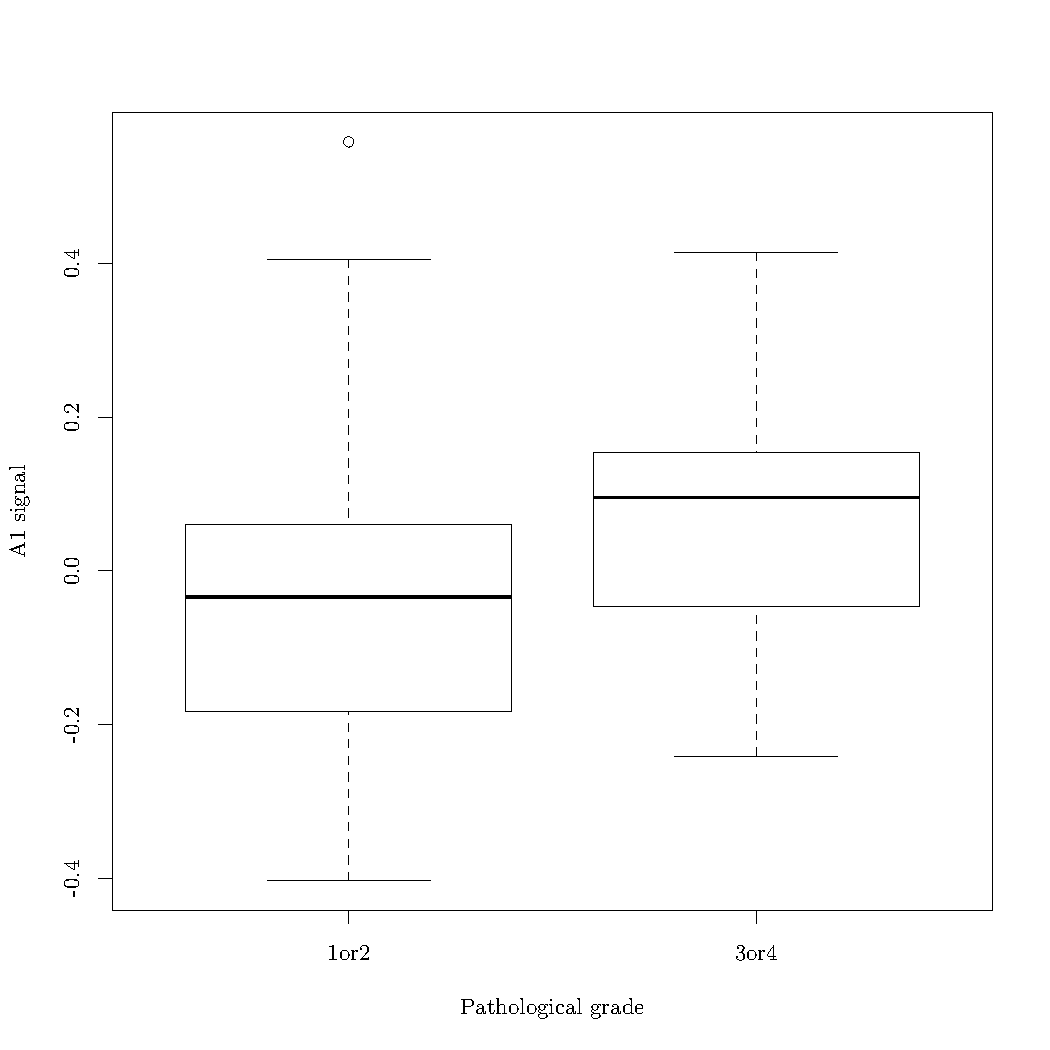
\includegraphics[width=\maxwidth]{figure/nmf-msigdb-cor-plots-1} 

}


\begin{kframe}\begin{alltt}
\hlkwd{heatmap.2}\hlstd{(nmf.final.msigdb.corr[, temp.sel_cols],} \hlkwc{trace} \hlstd{=} \hlstr{"none"}\hlstd{,} \hlkwc{scale} \hlstd{=} \hlstr{"none"}\hlstd{,}
    \hlkwc{useRaster} \hlstd{=} \hlnum{TRUE}\hlstd{,} \hlkwc{col} \hlstd{=} \hlkwd{brewer.pal}\hlstd{(}\hlnum{3}\hlstd{,} \hlstr{"PiYG"}\hlstd{),} \hlkwc{breaks} \hlstd{=} \hlkwd{c}\hlstd{(}\hlopt{-}\hlnum{1}\hlstd{,} \hlopt{-}\hlstd{sig.corr.threshold,}
        \hlstd{sig.corr.threshold,} \hlnum{1}\hlstd{))}
\end{alltt}
\end{kframe}

{\centering 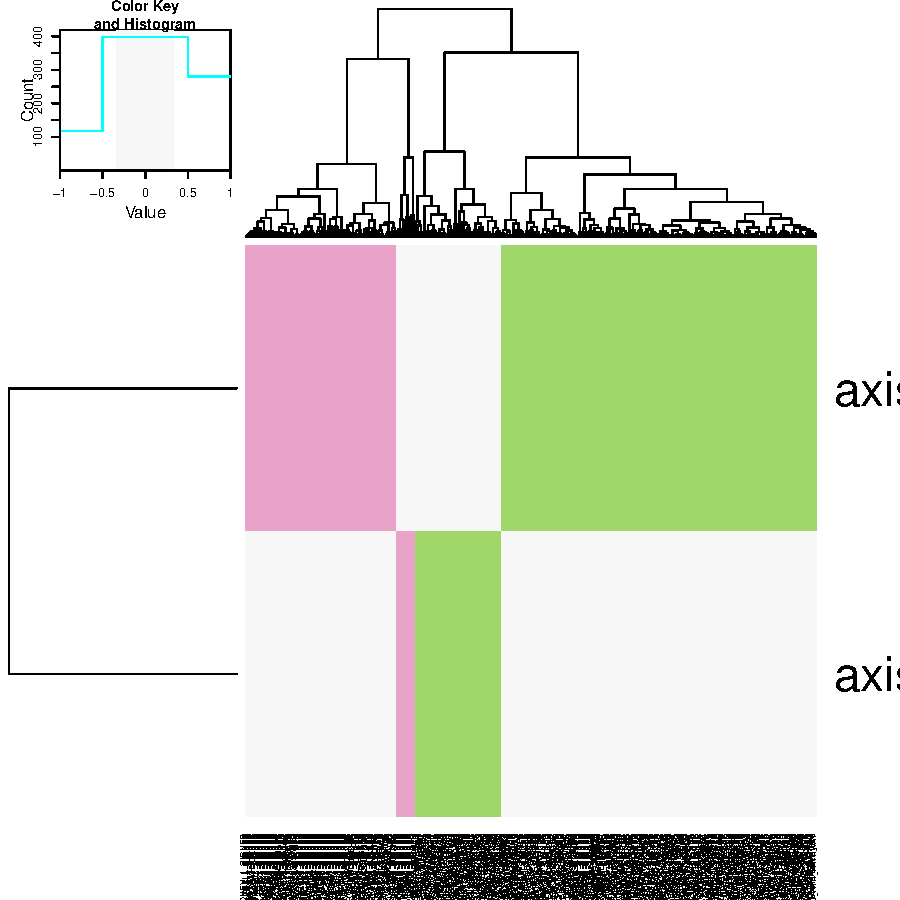
\includegraphics[width=\maxwidth]{figure/nmf-msigdb-cor-plots-2} 

}


\begin{kframe}\begin{alltt}
\hlstd{cpv.pvals} \hlkwb{=} \hlkwd{apply}\hlstd{(}\hlkwd{coef}\hlstd{(nmf.final),} \hlnum{1}\hlstd{,} \hlkwa{function}\hlstd{(}\hlkwc{mg}\hlstd{)} \hlkwd{sapply}\hlstd{(}\hlkwd{cbind}\hlstd{(cpvs.diag_dsd,}
    \hlkwc{purity} \hlstd{= samps}\hlopt{$}\hlstd{purity_qpure),} \hlkwa{function}\hlstd{(}\hlkwc{x}\hlstd{) \{}
    \hlstd{s} \hlkwb{=} \hlopt{!}\hlkwd{is.na}\hlstd{(mg)} \hlopt{& !}\hlkwd{is.na}\hlstd{(x)}
    \hlstd{x} \hlkwb{=} \hlstd{x[s]}
    \hlstd{mg} \hlkwb{=} \hlstd{mg[s]}
    \hlkwa{if} \hlstd{(}\hlkwd{any}\hlstd{(}\hlkwd{c}\hlstd{(}\hlstr{"numeric"}\hlstd{,} \hlstr{"integer"}\hlstd{)} \hlopt \hlkwd{class}\hlstd{(x))) \{}
        \hlkwd{return}\hlstd{(}\hlkwd{cor.test}\hlstd{(x, mg,} \hlkwc{method} \hlstd{=} \hlstr{"pearson"}\hlstd{)}\hlopt{$}\hlstd{p.value)}
    \hlstd{\}} \hlkwa{else if} \hlstd{(}\hlkwd{any}\hlstd{(}\hlkwd{c}\hlstd{(}\hlstr{"factor"}\hlstd{,} \hlstr{"ordered"}\hlstd{,} \hlstr{"logical"}\hlstd{)} \hlopt \hlkwd{class}\hlstd{(x))} \hlopt{&&} \hlkwd{length}\hlstd{(}\hlkwd{unique}\hlstd{(x))} \hlopt{>}
        \hlnum{1}\hlstd{) \{}
        \hlkwd{return}\hlstd{(}\hlkwd{anova}\hlstd{(}\hlkwd{lm}\hlstd{(mg} \hlopt{~} \hlstd{x))[,} \hlstr{"Pr(>F)"}\hlstd{][}\hlnum{1}\hlstd{])}
    \hlstd{\}}
    \hlnum{NA}
\hlstd{\}))}
\hlstd{cpv.pvals} \hlkwb{=} \hlstd{cpv.pvals[}\hlopt{!}\hlkwd{apply}\hlstd{(}\hlkwd{is.na}\hlstd{(cpv.pvals),} \hlnum{1}\hlstd{, all), ]}
\hlstd{cpv.pvals} \hlkwb{=} \hlstd{cpv.pvals[}\hlopt{!}\hlkwd{grepl}\hlstd{(}\hlstr{"^Surv\textbackslash{}\textbackslash{}."}\hlstd{,} \hlkwd{rownames}\hlstd{(cpv.pvals)), ]}
\hlstd{cpv.pvals} \hlkwb{=} \hlstd{cpv.pvals[}\hlopt{!}\hlkwd{grepl}\hlstd{(}\hlstr{"^Treat\textbackslash{}\textbackslash{}."}\hlstd{,} \hlkwd{rownames}\hlstd{(cpv.pvals)), ]}
\hlstd{cpv.pvals} \hlkwb{=} \hlstd{cpv.pvals[}\hlopt{!}\hlkwd{grepl}\hlstd{(}\hlstr{"^Path\textbackslash{}\textbackslash{}.Nodes"}\hlstd{,} \hlkwd{rownames}\hlstd{(cpv.pvals)), ]}
\hlstd{cpv.pvals} \hlkwb{=} \hlstd{cpv.pvals[}\hlopt{!}\hlkwd{grepl}\hlstd{(}\hlstr{"^Staging\textbackslash{}\textbackslash{}.Version"}\hlstd{,} \hlkwd{rownames}\hlstd{(cpv.pvals)), ]}
\hlstd{cpv.pvals} \hlkwb{=} \hlstd{cpv.pvals[}\hlopt{!}\hlkwd{grepl}\hlstd{(}\hlstr{"^History\textbackslash{}\textbackslash{}.Recurrence$"}\hlstd{,} \hlkwd{rownames}\hlstd{(cpv.pvals)),}
    \hlstd{]}
\hlstd{cpv.pvals} \hlkwb{=} \hlstd{cpv.pvals[}\hlopt{!}\hlkwd{grepl}\hlstd{(}\hlstr{"^History\textbackslash{}\textbackslash{}.Status$"}\hlstd{,} \hlkwd{rownames}\hlstd{(cpv.pvals)), ]}
\hlstd{cpv.pvals} \hlkwb{=} \hlstd{cpv.pvals[}\hlopt{!}\hlkwd{grepl}\hlstd{(}\hlstr{"^History\textbackslash{}\textbackslash{}.Death\textbackslash{}\textbackslash{}.Cause$"}\hlstd{,} \hlkwd{rownames}\hlstd{(cpv.pvals)),}
    \hlstd{]}
\hlstd{cpv.pvals} \hlkwb{=} \hlstd{cpv.pvals[}\hlopt{!}\hlkwd{grepl}\hlstd{(}\hlstr{"^Path\textbackslash{}\textbackslash{}.Grade$"}\hlstd{,} \hlkwd{rownames}\hlstd{(cpv.pvals)), ]}
\hlstd{cpv.pvals} \hlkwb{=} \hlstd{cpv.pvals[}\hlopt{!}\hlkwd{grepl}\hlstd{(}\hlstr{"^Path\textbackslash{}\textbackslash{}.TumourLocation$"}\hlstd{,} \hlkwd{rownames}\hlstd{(cpv.pvals)),}
    \hlstd{]}

\hlstd{temp} \hlkwb{=} \hlkwd{as.vector}\hlstd{(cpv.pvals)}
\hlstd{temp} \hlkwb{=} \hlkwd{p.adjust}\hlstd{(temp,} \hlstr{"holm"}\hlstd{)}
\hlstd{cpv.qvals} \hlkwb{=} \hlkwd{matrix}\hlstd{(temp,} \hlkwc{nrow} \hlstd{=} \hlkwd{nrow}\hlstd{(cpv.pvals))}
\hlkwd{rownames}\hlstd{(cpv.qvals)} \hlkwb{=} \hlkwd{rownames}\hlstd{(cpv.pvals)}
\hlkwd{colnames}\hlstd{(cpv.qvals)} \hlkwb{=} \hlkwd{colnames}\hlstd{(cpv.pvals)}
\hlstd{cpv.pvals}
\end{alltt}
\begin{verbatim}
##                                         [,1]      [,2]    [,3]     [,4]
## Patient.Gender                      0.138407 2.069e-02 0.72732 0.135009
## Patient.Ethnicity                   0.622781 7.244e-01 0.18976 0.765995
## History.Smoking.PackYears           0.348090 2.604e-01 0.73136 0.321908
## History.Diagnosis.AgeAtYears        0.881590 6.816e-01 0.49230 0.914690
## Path.HistoType.Subtype              0.893359 5.620e-01 0.22914 0.104016
## Path.TumourSizeMm                   0.940836 1.352e-01 0.70907 0.215133
## Path.Invasion.PN                    0.326270 6.452e-02 0.89694 0.509692
## Path.Invasion.VS                    0.626581 1.745e-01 0.93410 0.631215
## Staging.pM                          0.396481 3.624e-01 0.85889 0.135211
## Staging.pN                          0.731239 1.811e-01 0.62403 0.751373
## Staging.pT                          0.137691 5.530e-01 0.34901 0.064967
## Staging.Stage                       0.038185 2.195e-01 0.60239 0.089545
## History.Recurrence.Site.Peritoneum  0.958146 5.285e-02 0.61695 0.281081
## History.Recurrence.Site.PancRemnant 0.551611 2.399e-01 0.01780 0.914636
## History.Recurrence.Site.PancBed     0.869281 3.251e-01 0.66994 0.475247
## History.Recurrence.Site.Other       0.682468 2.960e-01 0.70889 0.003592
## History.Recurrence.Site.Omentum     0.120811 2.790e-01 0.95417 0.784937
## History.Recurrence.Site.Mesentery   0.502274 2.771e-01 0.78581 0.707436
## History.Recurrence.Site.LymphNodes  0.331799 9.865e-01 0.63649 0.014826
## History.Recurrence.Site.Lung        0.488661 2.979e-01 0.55622 0.748563
## History.Recurrence.Site.Liver       0.129400 4.693e-02 0.06894 0.547538
## History.Recurrence.Site.Brain       0.774503 2.987e-02 0.63502 0.971582
## History.Recurrence.Site.Bone        0.782178 8.047e-01 0.98003 0.854252
## Path.Grade.Coarse                   0.006438 5.655e-03 0.36879 0.129514
## Path.TumourLocation.Coarse          0.469811 2.301e-01 0.07124 0.567640
## purity                              0.047335 1.512e-05 0.09329 0.463260
##                                          [,5]      [,6]
## Patient.Gender                      3.733e-01 0.0387623
## Patient.Ethnicity                   9.939e-01 0.0191721
## History.Smoking.PackYears           5.061e-01 0.4738379
## History.Diagnosis.AgeAtYears        7.512e-01 0.7515763
## Path.HistoType.Subtype              5.660e-01 0.0595163
## Path.TumourSizeMm                   8.154e-01 0.4037090
## Path.Invasion.PN                    6.422e-02 0.8347923
## Path.Invasion.VS                    7.806e-01 0.0862062
## Staging.pM                          7.803e-01 0.2488073
## Staging.pN                          1.124e-01 0.5892122
## Staging.pT                          6.051e-01 0.4778634
## Staging.Stage                       1.922e-01 0.4591937
## History.Recurrence.Site.Peritoneum  8.085e-01 0.0275532
## History.Recurrence.Site.PancRemnant 6.621e-01 0.2693233
## History.Recurrence.Site.PancBed     9.389e-01 0.9235058
## History.Recurrence.Site.Other       6.915e-02 0.1710832
## History.Recurrence.Site.Omentum     3.392e-01 0.0596320
## History.Recurrence.Site.Mesentery   4.057e-01 0.1203379
## History.Recurrence.Site.LymphNodes  3.963e-01 0.7818857
## History.Recurrence.Site.Lung        2.854e-02 0.0896567
## History.Recurrence.Site.Liver       3.725e-01 0.4265668
## History.Recurrence.Site.Brain       2.810e-01 0.3088652
## History.Recurrence.Site.Bone        4.605e-01 0.0952863
## Path.Grade.Coarse                   1.468e-02 0.0001869
## Path.TumourLocation.Coarse          1.092e-01 0.1813727
## purity                              1.375e-05 0.1063724
\end{verbatim}
\begin{alltt}
\hlstd{cpv.qvals}
\end{alltt}
\begin{verbatim}
##                                       [,1]     [,2] [,3]   [,4]     [,5]
## Patient.Gender                      1.0000 1.000000    1 1.0000 1.000000
## Patient.Ethnicity                   1.0000 1.000000    1 1.0000 1.000000
## History.Smoking.PackYears           1.0000 1.000000    1 1.0000 1.000000
## History.Diagnosis.AgeAtYears        1.0000 1.000000    1 1.0000 1.000000
## Path.HistoType.Subtype              1.0000 1.000000    1 1.0000 1.000000
## Path.TumourSizeMm                   1.0000 1.000000    1 1.0000 1.000000
## Path.Invasion.PN                    1.0000 1.000000    1 1.0000 1.000000
## Path.Invasion.VS                    1.0000 1.000000    1 1.0000 1.000000
## Staging.pM                          1.0000 1.000000    1 1.0000 1.000000
## Staging.pN                          1.0000 1.000000    1 1.0000 1.000000
## Staging.pT                          1.0000 1.000000    1 1.0000 1.000000
## Staging.Stage                       1.0000 1.000000    1 1.0000 1.000000
## History.Recurrence.Site.Peritoneum  1.0000 1.000000    1 1.0000 1.000000
## History.Recurrence.Site.PancRemnant 1.0000 1.000000    1 1.0000 1.000000
## History.Recurrence.Site.PancBed     1.0000 1.000000    1 1.0000 1.000000
## History.Recurrence.Site.Other       1.0000 1.000000    1 0.5496 1.000000
## History.Recurrence.Site.Omentum     1.0000 1.000000    1 1.0000 1.000000
## History.Recurrence.Site.Mesentery   1.0000 1.000000    1 1.0000 1.000000
## History.Recurrence.Site.LymphNodes  1.0000 1.000000    1 1.0000 1.000000
## History.Recurrence.Site.Lung        1.0000 1.000000    1 1.0000 1.000000
## History.Recurrence.Site.Liver       1.0000 1.000000    1 1.0000 1.000000
## History.Recurrence.Site.Brain       1.0000 1.000000    1 1.0000 1.000000
## History.Recurrence.Site.Bone        1.0000 1.000000    1 1.0000 1.000000
## Path.Grade.Coarse                   0.9721 0.859520    1 1.0000 1.000000
## Path.TumourLocation.Coarse          1.0000 1.000000    1 1.0000 1.000000
## purity                              1.0000 0.002343    1 1.0000 0.002145
##                                        [,6]
## Patient.Gender                      1.00000
## Patient.Ethnicity                   1.00000
## History.Smoking.PackYears           1.00000
## History.Diagnosis.AgeAtYears        1.00000
## Path.HistoType.Subtype              1.00000
## Path.TumourSizeMm                   1.00000
## Path.Invasion.PN                    1.00000
## Path.Invasion.VS                    1.00000
## Staging.pM                          1.00000
## Staging.pN                          1.00000
## Staging.pT                          1.00000
## Staging.Stage                       1.00000
## History.Recurrence.Site.Peritoneum  1.00000
## History.Recurrence.Site.PancRemnant 1.00000
## History.Recurrence.Site.PancBed     1.00000
## History.Recurrence.Site.Other       1.00000
## History.Recurrence.Site.Omentum     1.00000
## History.Recurrence.Site.Mesentery   1.00000
## History.Recurrence.Site.LymphNodes  1.00000
## History.Recurrence.Site.Lung        1.00000
## History.Recurrence.Site.Liver       1.00000
## History.Recurrence.Site.Brain       1.00000
## History.Recurrence.Site.Bone        1.00000
## Path.Grade.Coarse                   0.02879
## Path.TumourLocation.Coarse          1.00000
## purity                              1.00000
\end{verbatim}
\begin{alltt}
\hlstd{cpv.pvals} \hlkwb{=} \hlstd{cpv.pvals[,} \hlkwd{c}\hlstd{(}\hlnum{1}\hlstd{,} \hlnum{2}\hlstd{,} \hlnum{5}\hlstd{,} \hlnum{6}\hlstd{)]}
\hlstd{temp} \hlkwb{=} \hlkwd{as.vector}\hlstd{(cpv.pvals)}
\hlstd{temp} \hlkwb{=} \hlkwd{p.adjust}\hlstd{(temp,} \hlstr{"holm"}\hlstd{)}
\hlstd{cpv.qvals} \hlkwb{=} \hlkwd{matrix}\hlstd{(temp,} \hlkwc{nrow} \hlstd{=} \hlkwd{nrow}\hlstd{(cpv.pvals))}
\hlkwd{rownames}\hlstd{(cpv.qvals)} \hlkwb{=} \hlkwd{rownames}\hlstd{(cpv.pvals)}
\hlkwd{colnames}\hlstd{(cpv.qvals)} \hlkwb{=} \hlkwd{colnames}\hlstd{(cpv.pvals)}
\hlstd{cpv.pvals}
\end{alltt}
\begin{verbatim}
##                                         [,1]      [,2]      [,3]      [,4]
## Patient.Gender                      0.138407 2.069e-02 3.733e-01 0.0387623
## Patient.Ethnicity                   0.622781 7.244e-01 9.939e-01 0.0191721
## History.Smoking.PackYears           0.348090 2.604e-01 5.061e-01 0.4738379
## History.Diagnosis.AgeAtYears        0.881590 6.816e-01 7.512e-01 0.7515763
## Path.HistoType.Subtype              0.893359 5.620e-01 5.660e-01 0.0595163
## Path.TumourSizeMm                   0.940836 1.352e-01 8.154e-01 0.4037090
## Path.Invasion.PN                    0.326270 6.452e-02 6.422e-02 0.8347923
## Path.Invasion.VS                    0.626581 1.745e-01 7.806e-01 0.0862062
## Staging.pM                          0.396481 3.624e-01 7.803e-01 0.2488073
## Staging.pN                          0.731239 1.811e-01 1.124e-01 0.5892122
## Staging.pT                          0.137691 5.530e-01 6.051e-01 0.4778634
## Staging.Stage                       0.038185 2.195e-01 1.922e-01 0.4591937
## History.Recurrence.Site.Peritoneum  0.958146 5.285e-02 8.085e-01 0.0275532
## History.Recurrence.Site.PancRemnant 0.551611 2.399e-01 6.621e-01 0.2693233
## History.Recurrence.Site.PancBed     0.869281 3.251e-01 9.389e-01 0.9235058
## History.Recurrence.Site.Other       0.682468 2.960e-01 6.915e-02 0.1710832
## History.Recurrence.Site.Omentum     0.120811 2.790e-01 3.392e-01 0.0596320
## History.Recurrence.Site.Mesentery   0.502274 2.771e-01 4.057e-01 0.1203379
## History.Recurrence.Site.LymphNodes  0.331799 9.865e-01 3.963e-01 0.7818857
## History.Recurrence.Site.Lung        0.488661 2.979e-01 2.854e-02 0.0896567
## History.Recurrence.Site.Liver       0.129400 4.693e-02 3.725e-01 0.4265668
## History.Recurrence.Site.Brain       0.774503 2.987e-02 2.810e-01 0.3088652
## History.Recurrence.Site.Bone        0.782178 8.047e-01 4.605e-01 0.0952863
## Path.Grade.Coarse                   0.006438 5.655e-03 1.468e-02 0.0001869
## Path.TumourLocation.Coarse          0.469811 2.301e-01 1.092e-01 0.1813727
## purity                              0.047335 1.512e-05 1.375e-05 0.1063724
\end{verbatim}
\begin{alltt}
\hlstd{cpv.qvals}
\end{alltt}
\begin{verbatim}
##                                       [,1]     [,2]    [,3]    [,4]
## Patient.Gender                      1.0000 1.000000 1.00000 1.00000
## Patient.Ethnicity                   1.0000 1.000000 1.00000 1.00000
## History.Smoking.PackYears           1.0000 1.000000 1.00000 1.00000
## History.Diagnosis.AgeAtYears        1.0000 1.000000 1.00000 1.00000
## Path.HistoType.Subtype              1.0000 1.000000 1.00000 1.00000
## Path.TumourSizeMm                   1.0000 1.000000 1.00000 1.00000
## Path.Invasion.PN                    1.0000 1.000000 1.00000 1.00000
## Path.Invasion.VS                    1.0000 1.000000 1.00000 1.00000
## Staging.pM                          1.0000 1.000000 1.00000 1.00000
## Staging.pN                          1.0000 1.000000 1.00000 1.00000
## Staging.pT                          1.0000 1.000000 1.00000 1.00000
## Staging.Stage                       1.0000 1.000000 1.00000 1.00000
## History.Recurrence.Site.Peritoneum  1.0000 1.000000 1.00000 1.00000
## History.Recurrence.Site.PancRemnant 1.0000 1.000000 1.00000 1.00000
## History.Recurrence.Site.PancBed     1.0000 1.000000 1.00000 1.00000
## History.Recurrence.Site.Other       1.0000 1.000000 1.00000 1.00000
## History.Recurrence.Site.Omentum     1.0000 1.000000 1.00000 1.00000
## History.Recurrence.Site.Mesentery   1.0000 1.000000 1.00000 1.00000
## History.Recurrence.Site.LymphNodes  1.0000 1.000000 1.00000 1.00000
## History.Recurrence.Site.Lung        1.0000 1.000000 1.00000 1.00000
## History.Recurrence.Site.Liver       1.0000 1.000000 1.00000 1.00000
## History.Recurrence.Site.Brain       1.0000 1.000000 1.00000 1.00000
## History.Recurrence.Site.Bone        1.0000 1.000000 1.00000 1.00000
## Path.Grade.Coarse                   0.6438 0.571128 1.00000 0.01907
## Path.TumourLocation.Coarse          1.0000 1.000000 1.00000 1.00000
## purity                              1.0000 0.001557 0.00143 1.00000
\end{verbatim}
\begin{alltt}
\hlkwd{boxplot}\hlstd{(}\hlkwd{coef}\hlstd{(nmf.final)[}\hlnum{6}\hlstd{, ]} \hlopt{~} \hlstd{cpvs.diag_dsd}\hlopt{$}\hlstd{Path.Grade.Coarse)}
\end{alltt}
\end{kframe}

{\centering 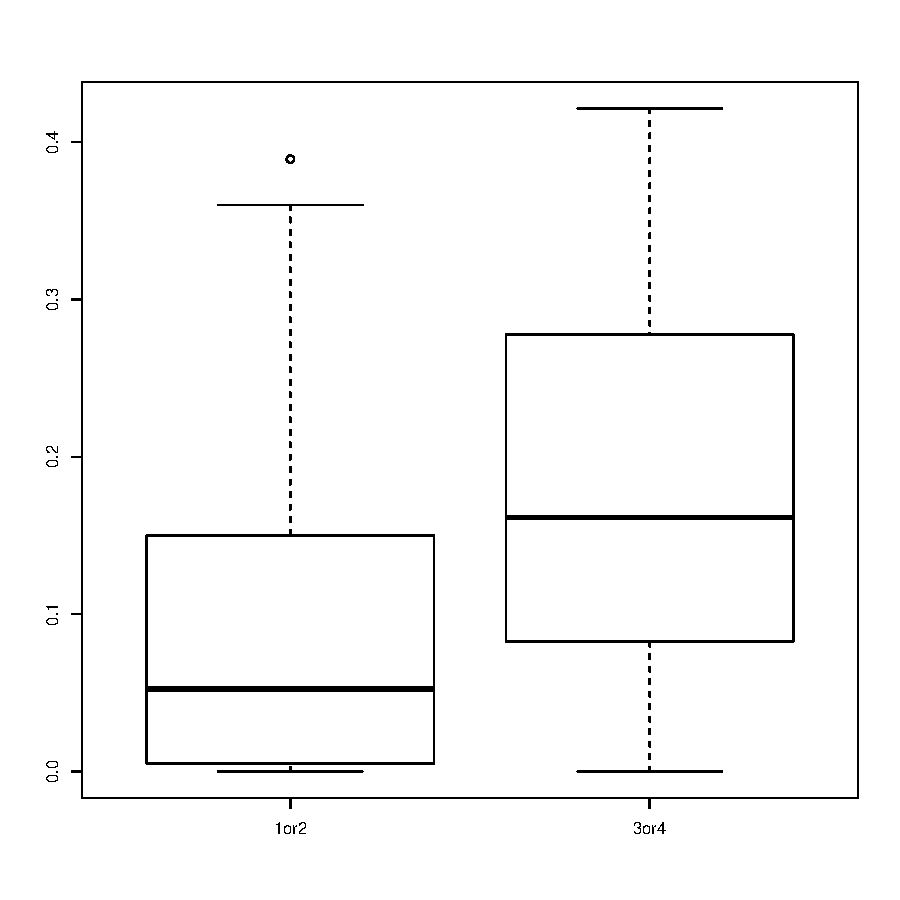
\includegraphics[width=\maxwidth]{figure/nmf-msigdb-cor-plots-3} 

}


\begin{kframe}\begin{alltt}
\hlcom{# plot(coef(nmf.final)[1,] ~ samps$purity_qpure) plot(coef(nmf.final)[2,] ~}
\hlcom{# samps$purity_qpure) plot(coef(nmf.final)[3,] ~ samps$purity_qpure)}
\hlcom{# plot(coef(nmf.final)[4,] ~ samps$purity_qpure) plot(coef(nmf.final)[5,] ~}
\hlcom{# samps$purity_qpure) plot(coef(nmf.final)[6,] ~ samps$purity_qpure)}

\hlkwd{apply}\hlstd{(}\hlkwd{coef}\hlstd{(nmf.final),} \hlnum{1}\hlstd{,} \hlkwa{function}\hlstd{(}\hlkwc{c1}\hlstd{)} \hlkwd{cor.test}\hlstd{(c1, samps}\hlopt{$}\hlstd{purity_qpure,} \hlkwc{method} \hlstd{=} \hlstr{"kendall"}\hlstd{))}
\end{alltt}
\begin{verbatim}
## [[1]]
## 
## 	Kendall's rank correlation tau
## 
## data:  c1 and samps$purity_qpure
## z = 2.503, p-value = 0.01233
## alternative hypothesis: true tau is not equal to 0
## sample estimates:
##    tau 
## 0.1934 
## 
## 
## [[2]]
## 
## 	Kendall's rank correlation tau
## 
## data:  c1 and samps$purity_qpure
## z = 3.915, p-value = 9.044e-05
## alternative hypothesis: true tau is not equal to 0
## sample estimates:
##    tau 
## 0.3031 
## 
## 
## [[3]]
## 
## 	Kendall's rank correlation tau
## 
## data:  c1 and samps$purity_qpure
## z = 0.2677, p-value = 0.789
## alternative hypothesis: true tau is not equal to 0
## sample estimates:
##     tau 
## 0.02075 
## 
## 
## [[4]]
## 
## 	Kendall's rank correlation tau
## 
## data:  c1 and samps$purity_qpure
## z = -0.7204, p-value = 0.4713
## alternative hypothesis: true tau is not equal to 0
## sample estimates:
##     tau 
## -0.0572 
## 
## 
## [[5]]
## 
## 	Kendall's rank correlation tau
## 
## data:  c1 and samps$purity_qpure
## z = -3.714, p-value = 0.0002043
## alternative hypothesis: true tau is not equal to 0
## sample estimates:
##     tau 
## -0.2882 
## 
## 
## [[6]]
## 
## 	Kendall's rank correlation tau
## 
## data:  c1 and samps$purity_qpure
## z = -2.15, p-value = 0.03156
## alternative hypothesis: true tau is not equal to 0
## sample estimates:
##     tau 
## -0.1686
\end{verbatim}
\begin{alltt}
\hlkwd{p.adjust}\hlstd{(}\hlkwd{apply}\hlstd{(}\hlkwd{coef}\hlstd{(nmf.final),} \hlnum{1}\hlstd{,} \hlkwa{function}\hlstd{(}\hlkwc{c1}\hlstd{)} \hlkwd{cor.test}\hlstd{(c1, samps}\hlopt{$}\hlstd{purity_qpure,}
    \hlkwc{method} \hlstd{=} \hlstr{"kendall"}\hlstd{)}\hlopt{$}\hlstd{p.value),} \hlstr{"BY"}\hlstd{)}
\end{alltt}
\begin{verbatim}
## [1] 0.060403 0.001329 1.000000 1.000000 0.001501 0.115993
\end{verbatim}
\begin{alltt}
\hlcom{# termplot(lm(coef(nmf.final)[6,] ~ cpvs.diag_dsd$Path.Grade.Coarse), se =}
\hlcom{# TRUE, rug = TRUE)}
\hlkwd{lm}\hlstd{(}\hlkwd{coef}\hlstd{(nmf.final)[}\hlnum{6}\hlstd{, ]} \hlopt{~} \hlstd{cpvs.diag_dsd}\hlopt{$}\hlstd{Path.Grade.Coarse)}
\end{alltt}
\begin{verbatim}
## 
## Call:
## lm(formula = coef(nmf.final)[6, ] ~ cpvs.diag_dsd$Path.Grade.Coarse)
## 
## Coefficients:
##                       (Intercept)  cpvs.diag_dsd$Path.Grade.Coarse.L  
##                            0.1353                             0.0623
\end{verbatim}
\begin{alltt}
\hlkwd{summary}\hlstd{(}\hlkwd{lm}\hlstd{(}\hlkwd{coef}\hlstd{(nmf.final)[}\hlnum{6}\hlstd{, ]} \hlopt{~} \hlstd{cpvs.diag_dsd}\hlopt{$}\hlstd{Path.Grade.Coarse))}
\end{alltt}
\begin{verbatim}
## 
## Call:
## lm(formula = coef(nmf.final)[6, ] ~ cpvs.diag_dsd$Path.Grade.Coarse)
## 
## Residuals:
##     Min      1Q  Median      3Q     Max 
## -0.1793 -0.0878 -0.0365  0.0655  0.2979 
## 
## Coefficients:
##                                   Estimate Std. Error t value Pr(>|t|)
## (Intercept)                         0.1353     0.0114   11.89  < 2e-16
## cpvs.diag_dsd$Path.Grade.Coarse.L   0.0623     0.0161    3.87  0.00019
## 
## Residual standard error: 0.107 on 108 degrees of freedom
## Multiple R-squared:  0.122,	Adjusted R-squared:  0.114 
## F-statistic:   15 on 1 and 108 DF,  p-value: 0.000187
\end{verbatim}
\begin{alltt}
\hlkwd{anova}\hlstd{(}\hlkwd{lm}\hlstd{(}\hlkwd{coef}\hlstd{(nmf.final)[}\hlnum{6}\hlstd{, ]} \hlopt{~} \hlstd{cpvs.diag_dsd}\hlopt{$}\hlstd{Path.Grade.Coarse))}
\end{alltt}
\begin{verbatim}
## Analysis of Variance Table
## 
## Response: coef(nmf.final)[6, ]
##                                  Df Sum Sq Mean Sq F value  Pr(>F)
## cpvs.diag_dsd$Path.Grade.Coarse   1  0.173  0.1727      15 0.00019
## Residuals                       108  1.245  0.0115
\end{verbatim}
\end{kframe}
\end{knitrout}


\begin{knitrout}
\definecolor{shadecolor}{rgb}{0.969, 0.969, 0.969}\color{fgcolor}\begin{kframe}
\begin{alltt}
\hlstd{temp.sig_id} \hlkwb{=} \hlkwd{colnames}\hlstd{(nmf.final.msigdb.corr)}
\hlstd{temp.sig_class} \hlkwb{=} \hlkwd{gsub}\hlstd{(}\hlstr{"\textbackslash{}\textbackslash{}..*"}\hlstd{,} \hlstr{""}\hlstd{, temp.sig_id)}
\hlstd{temp.nsigs} \hlkwb{=} \hlkwd{length}\hlstd{(temp.sig_id)}
\hlstd{temp.nmeta} \hlkwb{=} \hlkwd{nrow}\hlstd{(nmf.final.msigdb.corr)}
\hlstd{tables} \hlkwb{=} \hlkwd{lapply}\hlstd{(}\hlnum{1}\hlopt{:}\hlstd{temp.nmeta,} \hlkwa{function}\hlstd{(}\hlkwc{metagene_i}\hlstd{) \{}
    \hlkwd{tapply}\hlstd{(}\hlnum{1}\hlopt{:}\hlstd{temp.nsigs, temp.sig_class,} \hlkwa{function}\hlstd{(}\hlkwc{sig_class_is}\hlstd{) \{}
        \hlstd{all_cors} \hlkwb{=} \hlstd{nmf.final.msigdb.corr[, sig_class_is]}
        \hlstd{this_cors} \hlkwb{=} \hlstd{all_cors[metagene_i, ]}
        \hlstd{this_ids} \hlkwb{=} \hlstd{temp.sig_id[sig_class_is]}

        \hlstd{all_sig_cors} \hlkwb{=} \hlkwd{abs}\hlstd{(all_cors)} \hlopt{>=} \hlstd{sig.corr.threshold}
        \hlstd{this_sig_cors} \hlkwb{=} \hlstd{all_sig_cors[metagene_i, ]}

        \hlstd{sigs_to_report} \hlkwb{=} \hlkwd{which}\hlstd{(this_sig_cors)}

        \hlkwa{if} \hlstd{(}\hlkwd{length}\hlstd{(sigs_to_report)} \hlopt{==} \hlnum{0}\hlstd{) \{}
            \hlstd{table} \hlkwb{=} \hlkwd{data.frame}\hlstd{(}\hlkwc{GeneSet} \hlstd{=} \hlkwd{c}\hlstd{(),} \hlkwc{Correlation} \hlstd{=} \hlkwd{c}\hlstd{(),} \hlkwc{Metagenes} \hlstd{=} \hlkwd{c}\hlstd{())}
        \hlstd{\}} \hlkwa{else} \hlstd{\{}
            \hlstd{table} \hlkwb{=} \hlkwd{data.frame}\hlstd{(}\hlkwc{GeneSet} \hlstd{= this_ids[sigs_to_report],} \hlkwc{Correlation} \hlstd{= this_cors[sigs_to_report],}
                \hlkwc{Metagenes} \hlstd{=} \hlkwd{apply}\hlstd{(all_cors[, sigs_to_report,} \hlkwc{drop} \hlstd{=} \hlnum{FALSE}\hlstd{],}
                  \hlnum{2}\hlstd{,} \hlkwa{function}\hlstd{(}\hlkwc{cors}\hlstd{) \{}
                    \hlstd{sel} \hlkwb{=} \hlkwd{abs}\hlstd{(cors)} \hlopt{>=} \hlstd{sig.corr.threshold}
                    \hlcom{# A positive number implies that positive GSVA signal is associated with}
                    \hlcom{# worse prognosis}
                    \hlkwd{paste}\hlstd{(}\hlkwd{which}\hlstd{(sel)} \hlopt{*} \hlkwd{sign}\hlstd{(cors[}\hlkwd{which}\hlstd{(sel)]),} \hlkwc{collapse} \hlstd{=} \hlstr{","}\hlstd{)}
                  \hlstd{\}))}
            \hlstd{table} \hlkwb{=} \hlstd{table[}\hlkwd{order}\hlstd{(}\hlopt{-}\hlstd{(table}\hlopt{$}\hlstd{Correlation)), ]}
            \hlkwd{rownames}\hlstd{(table)} \hlkwb{<-} \hlkwa{NULL}
        \hlstd{\}}
        \hlstd{table}
    \hlstd{\},} \hlkwc{simplify} \hlstd{=} \hlnum{FALSE}\hlstd{)}
\hlstd{\})}
\hlstd{tables}
\end{alltt}
\begin{verbatim}
## [[1]]
## [[1]]$c1
## data frame with 0 columns and 0 rows
## 
## [[1]]$c2
##                                                                                                                                                                                                                                                                                                                                                   GeneSet
## 1                                                                                                                                                                                                                                                                                                                      c2.WU_APOPTOSIS_BY_CDKN1A_VIA_TP53
## 2                                                                                                                                                                                        c2.AMUNDSON_GAMMA_RADIATION_RESPONSE/c4.GNF2_CDC20/c4.GNF2_CDC2/c4.GNF2_CENPE/c4.GNF2_CENPF/c4.GNF2_CCNA2/c4.GNF2_CCNB2/c4.GNF2_H2AFX/c4.GNF2_HMMR/c4.GNF2_MKI67
## 3                                                                                                                                                                                                                                                                                   c2.FARMER_BREAST_CANCER_CLUSTER_2/c2.FINETTI_BREAST_CANCER_KINOME_RED
## 4                                                                                                                                                                                                                                                                  c2.WHITEFORD_PEDIATRIC_CANCER_MARKERS/c2.CHANG_CYCLING_GENES/c4.MODULE_54/c4.MODULE_57
## 5                                                                                                                                                                                                                                                                                                                       c2.GAVIN_FOXP3_TARGETS_CLUSTER_P6
## 6                                                                                                                                                                                         c2.EGUCHI_CELL_CYCLE_RB1_TARGETS/c2.ROSTY_CERVICAL_CANCER_PROLIFERATION_CLUSTER/c4.GNF2_BUB1/c4.GNF2_ESPL1/c4.GNF2_PCNA/c4.GNF2_RRM2/c4.GNF2_BUB1B/c4.GNF2_MCM4
## 7                                                                                                                                                                                                                                                                   c2.GOBERT_OLIGODENDROCYTE_DIFFERENTIATION_SIGNED/c2.MARSON_BOUND_BY_E2F4_UNSTIMULATED
## 8                                                                                                                                                                                                                                                                                                           c2.SOTIRIOU_BREAST_CANCER_GRADE_1_VS_3_SIGNED
## 9                                                                                                                                                                                                                                           c2.KONG_E2F3_TARGETS/c2.ZHOU_CELL_CYCLE_GENES_IN_IR_RESPONSE_6HR/c2.ZHOU_CELL_CYCLE_GENES_IN_IR_RESPONSE_24HR
## 10                                                                                                                                                                                                     c2.REACTOME_ACTIVATION_OF_THE_PRE_REPLICATIVE_COMPLEX/c2.REACTOME_ACTIVATION_OF_ATR_IN_RESPONSE_TO_REPLICATION_STRESS/c2.REACTOME_G2_M_CHECKPOINTS
## 11                                                                                                                                                                                                                                                                                                                      c2.RHODES_UNDIFFERENTIATED_CANCER
## 12                                                                                                                                                                                                                                                                                                  c2.REACTOME_CELL_CYCLE/c2.REACTOME_CELL_CYCLE_MITOTIC
## 13                                                                                                                                                                                                                                                                                                                       c2.REICHERT_MITOSIS_LIN9_TARGETS
## 14                                                                                                                                                                                                                                                                                                                c2.SHEDDEN_LUNG_CANCER_POOR_SURVIVAL_A6
## 15                                                                                                                                                                                                                                                                                                   c2.HOFFMANN_LARGE_TO_SMALL_PRE_BII_LYMPHOCYTE_SIGNED
## 16                                                                                                                                                                                                                                                                                                                    c2.BURTON_ADIPOGENESIS_PEAK_AT_24HR
## 17                                                                                                                                                                                                                                                                                                                                    c2.REN_BOUND_BY_E2F
## 18                                                                                                                                                                                                                                                                                                                                     c2.KEGG_CELL_CYCLE
## 19                                                                                                                                                                                                                                                                      c2.BURTON_ADIPOGENESIS_3/c2.ISHIDA_E2F_TARGETS/c2.WHITFIELD_CELL_CYCLE_LITERATURE
## 20                                                                                                                                                                                                                                                                                                                             c2.HU_GENOTOXIC_DAMAGE_4HR
## 21                                                                                                                                                                                                                                                                                      c2.KAMMINGA_EZH2_TARGETS/c4.GNF2_FEN1/c4.GNF2_RRM1/c4.GNF2_SMC4L1
## 22                                                                                                                                       c2.REACTOME_CELL_CYCLE_CHECKPOINTS/c2.REACTOME_G1_S_TRANSITION/c2.REACTOME_SYNTHESIS_OF_DNA/c2.REACTOME_MITOTIC_G1_G1_S_PHASES/c2.REACTOME_MITOTIC_M_M_G1_PHASES/c2.REACTOME_DNA_REPLICATION/c2.REACTOME_S_PHASE
## 23                                                                                                                                                                                                                                                                                                                             c2.BENPORATH_CYCLING_GENES
## 24                                                                                                                                                                                                                                                                                                                  c2.FOURNIER_ACINAR_DEVELOPMENT_LATE_2
## 25                                                                                                                                                                                                                                                                                                                     c2.ZHAN_MULTIPLE_MYELOMA_PR_SIGNED
## 26                                                                                                                                                                                                                                                                c2.PUJANA_XPRSS_INT_NETWORK/c2.PUJANA_BRCA2_PCC_NETWORK/c2.PUJANA_BRCA_CENTERED_NETWORK
## 27                                                                                                                                                                                                                                                                                                                       c2.REACTOME_MITOTIC_PROMETAPHASE
## 28                                                                                                                                                                                                                                                                                                                             c2.WHITFIELD_CELL_CYCLE_G2
## 29                                                                                                                                                                                                                                                                                                                    c2.BURTON_ADIPOGENESIS_PEAK_AT_16HR
## 30                                                                                                                                                                                                                                                                                                                           c2.WHITFIELD_CELL_CYCLE_G2_M
## 31                                                                                                                                                                                                                                                                                                                c2.BERENJENO_TRANSFORMED_BY_RHOA_SIGNED
## 32                                                                                                                                                                                                                                                                                                 c2.REACTOME_E2F_MEDIATED_REGULATION_OF_DNA_REPLICATION
## 33                                                                                                                                                                                                                                                                                                                          c2.KAUFFMANN_DNA_REPAIR_GENES
## 34                                                                                                                                                                                                                                                                                              c2.KEGG_DNA_REPLICATION/c2.REACTOME_DNA_STRAND_ELONGATION
## 35                                                                                                                                                                                                                                                                                                                                    c2.PID_FOXM1PATHWAY
## 36                                                                                                                                                                                                                                                                                                                                           c2.SU_TESTIS
## 37                                                                                                                                                                                                                                                                                       c2.REACTOME_CYCLIN_A_B1_ASSOCIATED_EVENTS_DURING_G2_M_TRANSITION
## 38                                                                                                                                                                                                                                                                                                                                     c2.PID_ATR_PATHWAY
## 39                                                                                                                                                                                                                                                                                                                             c2.BENPORATH_PROLIFERATION
## 40                                                                                                                                                                                                                                                                                                   c2.CHIANG_LIVER_CANCER_SUBCLASS_PROLIFERATION_SIGNED
## 41                                                                                                                                                                                                                                                                                                                     c2.KAUFFMANN_DNA_REPLICATION_GENES
## 42                                                                                                                                                                                                                                                                                                                                c2.OHASHI_AURKB_TARGETS
## 43                                                                                                                                                                                                                                                                                                                              c2.LE_EGR2_TARGETS_SIGNED
## 44                                                                                                                                                                                                                                                                                                                    c2.SONG_TARGETS_OF_IE86_CMV_PROTEIN
## 45                                                                                                                                                                                                                                                                                                                                      c2.BENPORATH_ES_1
## 46                                                                                                                                                                                                                                                                                                                c2.HONRADO_BREAST_CANCER_BRCA1_VS_BRCA2
## 47                                                                                                                                                                                                                                                                                                                                c2.BIOCARTA_MCM_PATHWAY
## 48                                                                                                                                                                                                                                                                                                                                  c2.KALMA_E2F1_TARGETS
## 49                                                                                                                                                                                                                                                                                                                                   c2.REACTOME_KINESINS
## 50                                                                                                                                                                                                                                                                                                                                c2.SHEPARD_BMYB_TARGETS
## 51                                                                                                                                                                                                                                                                                                             c2.REICHERT_G1S_REGULATORS_AS_PI3K_TARGETS
## 52                                                                                                                                                                                                                                                                                                         c2.MONTERO_THYROID_CANCER_POOR_SURVIVAL_SIGNED
## 53                                                                                                                                                                                                                                                                                                                 c2.REACTOME_G2_M_DNA_DAMAGE_CHECKPOINT
## 54                                                                                                                                                                                                                                                                                                                                 c2.BIOCARTA_G2_PATHWAY
## 55                                                                                                                                                                                                                                                                                                                           c2.REACTOME_UNWINDING_OF_DNA
## 56                                                                                                                                                                                                                                                                                                                                c2.PID_AURORA_B_PATHWAY
## 57                                                                                                                                                                                                                                                                                                     c2.SARRIO_EPITHELIAL_MESENCHYMAL_TRANSITION_SIGNED
## 58                                                                                                                                                                                                                                                                                                             c2.DUTERTRE_ESTRADIOL_RESPONSE_24HR_SIGNED
## 59                                                                                                                                                                                                                                                                                                                c2.REACTOME_G1_S_SPECIFIC_TRANSCRIPTION
## 60                                                                                                                                                                                                                                                                                                                            c2.ZHANG_TLX_TARGETS_SIGNED
## 61                                                                                                                                                                                                                                                                                                        c2.CHEMNITZ_RESPONSE_TO_PROSTAGLANDIN_E2_SIGNED
## 62                                                                                                                                                                                                                                                                                                   c2.FERREIRA_EWINGS_SARCOMA_UNSTABLE_VS_STABLE_SIGNED
## 63                                                                                                                                                                                                                                                                                                                c2.ZHENG_GLIOBLASTOMA_PLASTICITY_SIGNED
## 64                                                                                                                                                                                                                                                                                                        c2.WANG_METASTASIS_OF_BREAST_CANCER_ESR1_SIGNED
## 65                                                                                                                                                                                                                                                                                                                              c2.BIOCARTA_RANMS_PATHWAY
## 66                                                                                                                                                                                                                                                                                                                    c2.CHANG_CORE_SERUM_RESPONSE_SIGNED
## 67                                                                                                                                                                                                                                                                                                                                c2.PID_AURORA_A_PATHWAY
## 68                                                                                                                                                                                                                                c2.REACTOME_ORC1_REMOVAL_FROM_CHROMATIN/c2.REACTOME_M_G1_TRANSITION/c2.REACTOME_ASSEMBLY_OF_THE_PRE_REPLICATIVE_COMPLEX
## 69                                                                                                                                                                                                                                                                                            c2.RODRIGUES_THYROID_CARCINOMA_POORLY_DIFFERENTIATED_SIGNED
## 70                                                                                                                                                                                                                                                                                                                                    c2.PID_PLK1_PATHWAY
## 71                                                                                                                                                                                                                                                                                                                       c2.MORI_PRE_BI_LYMPHOCYTE_SIGNED
## 72                                                                                                                                                                                                                                                                                                                       c2.WONG_EMBRYONIC_STEM_CELL_CORE
## 73                                                                                                                                                                                                                                                                                                                  c2.KANG_DOXORUBICIN_RESISTANCE_SIGNED
## 74                                                                                                                                                                                                                                                                                                                                    c2.MUELLER_PLURINET
## 75                                                                                                                                                                                                                                                                                                                                    c2.PID_BARD1PATHWAY
## 76                                                                                                                                                                                                                                                                                c2.REACTOME_E2F_ENABLED_INHIBITION_OF_PRE_REPLICATION_COMPLEX_FORMATION
## 77                                                                                                                                                                                                                                                                                                       c2.RODRIGUES_THYROID_CARCINOMA_ANAPLASTIC_SIGNED
## 78                                                                                                                                                                                                                                                                                c2.REACTOME_LAGGING_STRAND_SYNTHESIS/c2.REACTOME_EXTENSION_OF_TELOMERES
## 79  c2.REACTOME_CYCLIN_E_ASSOCIATED_EVENTS_DURING_G1_S_TRANSITION_/c2.REACTOME_REGULATION_OF_MITOTIC_CELL_CYCLE/c2.REACTOME_APC_C_CDH1_MEDIATED_DEGRADATION_OF_CDC20_AND_OTHER_APC_C_CDH1_TARGETED_PROTEINS_IN_LATE_MITOSIS_EARLY_G1/c2.REACTOME_APC_C_CDC20_MEDIATED_DEGRADATION_OF_MITOTIC_PROTEINS/c2.REACTOME_SCFSKP2_MEDIATED_DEGRADATION_OF_P27_P21
## 80                                                                                                                                                                                                                                                                                                                c2.PUJANA_BREAST_CANCER_LIT_INT_NETWORK
## 81                                                                                                                                                                                                                                                                                                                                 c2.BIOCARTA_RB_PATHWAY
## 82                                                                                                                                                                                                                                                                                                                       c2.LEE_EARLY_T_LYMPHOCYTE_SIGNED
## 83                                                                                                                                                                                                                                                                                                                                c2.OHASHI_AURKA_TARGETS
## 84                                                                                                                                                                                                                                                                                                                        c2.SASAKI_ADULT_T_CELL_LEUKEMIA
## 85                                                                                                                                                                                                                                                                                                                                 c2.CROSBY_E2F4_TARGETS
## 86                                                                                                                                                                                                                                                                                                                        c2.RHODES_CANCER_META_SIGNATURE
## 87                                                                                                                                                                                                                                                                                                                          c2.BASAKI_YBX1_TARGETS_SIGNED
## 88                                                                                                                                                                                                                                                                                                                                 c2.KEGG_OOCYTE_MEIOSIS
## 89                                                                                                                                                                                                                                                                                                           c2.WINNEPENNINCKX_MELANOMA_METASTASIS_SIGNED
## 90                                                                                                                                                                                                                                                                                                                  c2.WAKASUGI_HAVE_ZNF143_BINDING_SITES
## 91                                                                                                                                                                                                                                                                                 c2.REACTOME_HIV_INFECTION/c2.REACTOME_HOST_INTERACTIONS_OF_HIV_FACTORS
## 92                                                                                                                                                                                                                                                                                                c2.PUJANA_BRCA1_PCC_NETWORK/c2.PUJANA_CHEK2_PCC_NETWORK
## 93                                                                                                                                                                                                                                                                                                                               c2.LY_AGING_PREMATURE_DN
## 94                                                                                                                                                                                                                                                                                                                              c2.REACTOME_POL_SWITCHING
## 95                                                                                                                                                                                                                                                                                                                             c2.GLINSKY_CANCER_DEATH_UP
## 96                                                                                                                                                                                                                                                                                                c2.REACTOME_ANTIVIRAL_MECHANISM_BY_IFN_STIMULATED_GENES
## 97                                                                                                                                                                                                                                                                                                    c2.NAKAMURA_TUMOR_ZONE_PERIPHERAL_VS_CENTRAL_SIGNED
## 98                                                                                                                                                                                                                                                                                                            c2.WEST_ADRENOCORTICAL_TUMOR_MARKERS_SIGNED
## 99                                                                                                                                                                                                                                                                                                             c2.BOYAULT_LIVER_CANCER_SUBCLASS_G3_SIGNED
## 100                                                                                                                                            c2.REACTOME_NEP_NS2_INTERACTS_WITH_THE_CELLULAR_EXPORT_MACHINERY/c2.REACTOME_TRANSPORT_OF_RIBONUCLEOPROTEINS_INTO_THE_HOST_NUCLEUS/c2.REACTOME_REGULATION_OF_GLUCOKINASE_BY_GLUCOKINASE_REGULATORY_PROTEIN
## 101                                                                                                                                                                                                                                                                                                                c2.TOYOTA_TARGETS_OF_MIR34B_AND_MIR34C
## 102                                                                                                                                                                                                                                                                                                               c2.GRADE_COLON_AND_RECTAL_CANCER_SIGNED
## 103                                                                                                                                                                                                                                                                                   c2.REACTOME_CHROMOSOME_MAINTENANCE/c2.REACTOME_TELOMERE_MAINTENANCE
## 104                                                                                                                                                                                                                                                                                                                         c2.BASSO_B_LYMPHOCYTE_NETWORK
## 105                                                                                                                                                                                                                                                                                                                           c2.CHEN_ETV5_TARGETS_TESTIS
## 106                                                                                                                                                                                                                                                                                                                   c2.WEST_ADRENOCORTICAL_TUMOR_SIGNED
## 107                                                                                                                                                                                                                                                                                                                                    c2.PID_ATM_PATHWAY
## 108                                                                                                                                                                                                                                                                                                c2.REACTOME_PROCESSIVE_SYNTHESIS_ON_THE_LAGGING_STRAND
## 109                                                                                                                                                                                                                                                                                                                      c2.RIZ_ERYTHROID_DIFFERENTIATION
## 110                                                                                                                                                                                                                                                                                           c2.REACTOME_INTERACTIONS_OF_VPR_WITH_HOST_CELLULAR_PROTEINS
## 111                                                                                                                                                                                                                                                                       c2.REACTOME_REGULATION_OF_MRNA_STABILITY_BY_PROTEINS_THAT_BIND_AU_RICH_ELEMENTS
## 112                                                                                                                                                                                                                                                                                                           c2.BOYAULT_LIVER_CANCER_SUBCLASS_G23_SIGNED
## 113                                                                                                                                                                                                                                                                                                                                c2.REACTOME_DNA_REPAIR
## 114                                                                                                                                                                                                                                                                                                                           c2.FERRANDO_HOX11_NEIGHBORS
## 115                                                                                                                                                                                                                                                                                                     c2.GRAHAM_CML_DIVIDING_VS_NORMAL_QUIESCENT_SIGNED
## 116                                                                                                                                                                                                                                                                            c2.REACTOME_TRANSPORT_OF_MATURE_MRNA_DERIVED_FROM_AN_INTRONLESS_TRANSCRIPT
## 117                                                                                                                                                                                                                                                                                                                        c2.WEI_MYCN_TARGETS_WITH_E_BOX
## 118                                                                                                                                                                                                                                                                                                                                 c2.SA_G2_AND_M_PHASES
## 119                                                                                                                                                                                                                                                                                                            c2.NAKAYAMA_SOFT_TISSUE_TUMORS_PCA2_SIGNED
## 120                                                                                                                                                                                                                                                                                                                 c2.VECCHI_GASTRIC_CANCER_EARLY_SIGNED
## 121                                                                                                                                                                                                                                                                                     c2.REACTOME_REPAIR_SYNTHESIS_FOR_GAP_FILLING_BY_DNA_POL_IN_TC_NER
## 122                                                                                                                                                                                                                                                                                                                   c2.BHATTACHARYA_EMBRYONIC_STEM_CELL
## 123                                                                                                                                                                                                                                                                                                         c2.KINSEY_TARGETS_OF_EWSR1_FLII_FUSION_SIGNED
## 124                                                                                                                                                                                                                                                                                                                                 c2.REACTOME_APOPTOSIS
## 125                                                                                                                                                                                                                                                                                   c2.REACTOME_HIV_LIFE_CYCLE/c2.REACTOME_LATE_PHASE_OF_HIV_LIFE_CYCLE
## 126                                                                                                                                                                                                                                                                                                              c2.REACTOME_METABOLISM_OF_NON_CODING_RNA
## 127                                                                                                                                                                                                                                                                                                               c2.MITSIADES_RESPONSE_TO_APLIDIN_SIGNED
## 128                                                                                                                                                                                                                                                                                                            c2.ALCALAY_AML_BY_NPM1_LOCALIZATION_SIGNED
## 129                                                                                                                                                                                                                                                                                                            c2.ODONNELL_TARGETS_OF_MYC_AND_TFRC_SIGNED
## 130                                                                                                                                                                                                                                                                                                            c2.CHUANG_OXIDATIVE_STRESS_RESPONSE_SIGNED
## 131                                                                                                                                                                                                                                                                                                                            c2.LEE_BMP2_TARGETS_SIGNED
## 132                                                                                                                                                                                                                                                                                                                             c2.LY_AGING_MIDDLE_SIGNED
## 133                                                                                                                                                                                                                                                                                                                 c2.LE_NEURONAL_DIFFERENTIATION_SIGNED
## 134                                                                                                                                                                                                                                                                                                    c2.WANG_RESPONSE_TO_GSK3_INHIBITOR_SB216763_SIGNED
## 135                                                                                                                                                                                                                                                                                                                              c2.MANALO_HYPOXIA_SIGNED
## 136                                                                                                                                                                                                                                                                                                                      c2.ZHANG_TLX_TARGETS_36HR_SIGNED
## 137                                                                                                                                                                                                                                                                                                   c2.SCIAN_CELL_CYCLE_TARGETS_OF_TP53_AND_TP73_SIGNED
## 138                                                                                                                                                                                                                                                                                                                c2.SMID_BREAST_CANCER_LUMINAL_A_SIGNED
## 139                                                                                                                                                                                                                                                                                                  c2.GRAHAM_NORMAL_QUIESCENT_VS_NORMAL_DIVIDING_SIGNED
## 140                                                                                                                                                                                                                                                                                                                  c2.CROONQUIST_IL6_DEPRIVATION_SIGNED
## 141                                                                                                                                                                                                                                                                                                                          c2.FUJII_YBX1_TARGETS_SIGNED
## 142                                                                                                                                                                                                                                                                                                  c2.STEIN_ESRRA_TARGETS_RESPONSIVE_TO_ESTROGEN_SIGNED
## 143                                                                                                                                                                                                                                                                                                                      c2.SIMBULAN_PARP1_TARGETS_SIGNED
## 144                                                                                                                                                                                                                                                                                                            c2.TARTE_PLASMA_CELL_VS_PLASMABLAST_SIGNED
## 145                                                                                                                                                                                                                                                                                                            c2.LI_WILMS_TUMOR_VS_FETAL_KIDNEY_1_SIGNED
## 146                                                                                                                                                                                                                                                                                                            c2.FOURNIER_ACINAR_DEVELOPMENT_LATE_SIGNED
## 147                                                                                                                                                                                                                                                                                                           c2.VANTVEER_BREAST_CANCER_METASTASIS_SIGNED
## 148                                                                                                                                                                                                                                                                                                          c2.MOLENAAR_TARGETS_OF_CCND1_AND_CDK4_SIGNED
## 149                                                                                                                                                                                                                                                                                                                       c2.HORIUCHI_WTAP_TARGETS_SIGNED
## 150                                                                                                                                                                                                                                                                                                                           c2.AFFAR_YY1_TARGETS_SIGNED
## 151                                                                                                                                                                                                                                                                                                              c2.KUMAMOTO_RESPONSE_TO_NUTLIN_3A_SIGNED
## 152                                                                                                                                                                                                                                                                                                                       c2.ODONNELL_TFRC_TARGETS_SIGNED
## 153                                                                                                                                                                                                                                                                                                            c2.NAKAMURA_CANCER_MICROENVIRONMENT_SIGNED
## 154                                                                                                                                                                                                                                                                                                                      c2.ZHANG_TLX_TARGETS_60HR_SIGNED
## 155                                                                                                                                                                                                                                                                                                                c2.TANG_SENESCENCE_TP53_TARGETS_SIGNED
## 156                                                                                                                                                                                                                                                                                                                            c2.RUIZ_TNC_TARGETS_SIGNED
## 157                                                                                                                                                                                                                                                                                                               c2.KOBAYASHI_EGFR_SIGNALING_24HR_SIGNED
##     Correlation Metagenes
## 1        0.7237         1
## 2        0.7139         1
## 3        0.7106         1
## 4        0.7103         1
## 5        0.7019         1
## 6        0.7002         1
## 7        0.6945         1
## 8        0.6858         1
## 9        0.6828         1
## 10       0.6825         1
## 11       0.6818         1
## 12       0.6808         1
## 13       0.6784         1
## 14       0.6748      1,-5
## 15       0.6691         1
## 16       0.6654         1
## 17       0.6597         1
## 18       0.6567         1
## 19       0.6537         1
## 20       0.6523         1
## 21       0.6500         1
## 22       0.6476         1
## 23       0.6473         1
## 24       0.6436      1,-5
## 25       0.6399      1,-5
## 26       0.6366         1
## 27       0.6359         1
## 28       0.6309         1
## 29       0.6188         1
## 30       0.6175         1
## 31       0.6172         1
## 32       0.6158         1
## 33       0.6158         1
## 34       0.6128         1
## 35       0.6128         1
## 36       0.6121         1
## 37       0.6115         1
## 38       0.6101         1
## 39       0.6095         1
## 40       0.6088         1
## 41       0.6088         1
## 42       0.6081         1
## 43       0.6068         1
## 44       0.6065         1
## 45       0.6048         1
## 46       0.6014         1
## 47       0.5981         1
## 48       0.5967         1
## 49       0.5964         1
## 50       0.5957         1
## 51       0.5941         1
## 52       0.5937         1
## 53       0.5937         1
## 54       0.5914         1
## 55       0.5904         1
## 56       0.5887         1
## 57       0.5854         1
## 58       0.5850         1
## 59       0.5820         1
## 60       0.5817         1
## 61       0.5813         1
## 62       0.5807         1
## 63       0.5800         1
## 64       0.5770         1
## 65       0.5766         1
## 66       0.5753      1,-5
## 67       0.5753         1
## 68       0.5746         1
## 69       0.5743      1,-5
## 70       0.5720         1
## 71       0.5713         1
## 72       0.5706         1
## 73       0.5679         1
## 74       0.5673         1
## 75       0.5666         1
## 76       0.5663         1
## 77       0.5612      1,-5
## 78       0.5612         1
## 79       0.5606         1
## 80       0.5602         1
## 81       0.5582         1
## 82       0.5552      1,-5
## 83       0.5552         1
## 84       0.5545         1
## 85       0.5529         1
## 86       0.5502         1
## 87       0.5489         1
## 88       0.5472         1
## 89       0.5468         1
## 90       0.5455         1
## 91       0.5425         1
## 92       0.5408         1
## 93       0.5385         1
## 94       0.5381         1
## 95       0.5375         1
## 96       0.5361         1
## 97       0.5348         1
## 98       0.5338         1
## 99       0.5318      1,-5
## 100      0.5311         1
## 101      0.5301         1
## 102      0.5291      1,-5
## 103      0.5281         1
## 104      0.5274         1
## 105      0.5271         1
## 106      0.5241      1,-5
## 107      0.5224         1
## 108      0.5221         1
## 109      0.5217         1
## 110      0.5187         1
## 111      0.5184         1
## 112      0.5177      1,-5
## 113      0.5174         1
## 114      0.5170         1
## 115      0.5167         1
## 116      0.5160         1
## 117      0.5150         1
## 118      0.5120         1
## 119      0.5113      1,-5
## 120      0.5113      1,-5
## 121      0.5113         1
## 122      0.5110         1
## 123      0.5100         1
## 124      0.5097         1
## 125      0.5090         1
## 126      0.5083         1
## 127     -0.5053        -1
## 128     -0.5080        -1
## 129     -0.5090        -1
## 130     -0.5100        -1
## 131     -0.5134        -1
## 132     -0.5134        -1
## 133     -0.5150      -1,5
## 134     -0.5187        -1
## 135     -0.5201        -1
## 136     -0.5274        -1
## 137     -0.5318        -1
## 138     -0.5351        -1
## 139     -0.5475        -1
## 140     -0.5495        -1
## 141     -0.5556        -1
## 142     -0.5582        -1
## 143     -0.5586        -1
## 144     -0.5699      -1,5
## 145     -0.5780        -1
## 146     -0.5877        -1
## 147     -0.5884        -1
## 148     -0.5954        -1
## 149     -0.5961        -1
## 150     -0.5994        -1
## 151     -0.6105        -1
## 152     -0.6128        -1
## 153     -0.6138        -1
## 154     -0.6165        -1
## 155     -0.6570        -1
## 156     -0.6594        -1
## 157     -0.6979        -1
## 
## [[1]]$c3
##                          GeneSet Correlation Metagenes
## 1                 c3.V$E2F_Q4_01      0.5401         1
## 2                 c3.V$E2F_Q6_01      0.5284         1
## 3 c3.V$E2F_Q3_01/c3.V$E2F1_Q4_01      0.5167         1
## 4      c3.SGCGSSAAA_V$E2F1DP2_01      0.5093         1
## 
## [[1]]$c4
##                                                                            GeneSet
## 1  c4.GNF2_RFC3/c4.GNF2_RFC4/c4.GNF2_SMC2L1/c4.GNF2_CKS1B/c4.GNF2_CKS2/c4.GNF2_TTK
## 2                                                                    c4.MORF_BUB1B
## 3                                                                    c4.MODULE_403
## 4                                                                     c4.MORF_FEN1
## 5                                                      c4.MODULE_125/c4.MODULE_158
## 6                                                                     c4.MODULE_17
## 7                                                                    c4.MODULE_320
## 8                                                                    c4.MODULE_126
## 9                                                                    c4.MORF_ESPL1
## 10                                                                   c4.MODULE_315
## 11                                                                   c4.MODULE_124
## 12                                                                   c4.MODULE_244
## 13                                                                    c4.GNF2_MSH2
## 14                                        c4.MODULE_98/c4.MODULE_198/c4.MODULE_252
## 15                                                                    c4.GNF2_MCM5
## 16                                                                   c4.MODULE_451
## 17                                                                    c4.MORF_BUB1
## 18                                                                   c4.MODULE_278
## 19                                                                    c4.MORF_CCNF
## 20                                                       c4.GNF2_PA2G4/c4.GNF2_RAN
## 21                                                       c4.MORF_RFC4/c4.MORF_RRM1
## 22                                                                    c4.GNF2_MSH6
## 23                                                                     c4.MORF_UNG
## 24                                                                   c4.MORF_DNMT1
## 25                                                     c4.MORF_BUB3/c4.MORF_RAD23A
## 26                                                                    c4.MORF_PCNA
## 27                                                                   c4.MODULE_337
## 28                                                                     c4.MODULE_8
##    Correlation Metagenes
## 1       0.7032         1
## 2       0.6517         1
## 3       0.6245         1
## 4       0.6239         1
## 5       0.6212         1
## 6       0.6175         1
## 7       0.6078         1
## 8       0.6061         1
## 9       0.6048         1
## 10      0.5998         1
## 11      0.5904         1
## 12      0.5904         1
## 13      0.5820         1
## 14      0.5787         1
## 15      0.5713         1
## 16      0.5643         1
## 17      0.5602         1
## 18      0.5545         1
## 19      0.5425         1
## 20      0.5348         1
## 21      0.5278         1
## 22      0.5244         1
## 23      0.5154         1
## 24      0.5117         1
## 25      0.5093         1
## 26      0.5063         1
## 27      0.5030      1,-5
## 28      0.5006         1
## 
## [[1]]$c5
##                                                                                  GeneSet
## 1                                 c5.M_PHASE/c5.MITOSIS/c5.M_PHASE_OF_MITOTIC_CELL_CYCLE
## 2                        c5.CELL_CYCLE_PROCESS/c5.MITOTIC_CELL_CYCLE/c5.CELL_CYCLE_PHASE
## 3                                                               c5.REGULATION_OF_MITOSIS
## 4                                                                             c5.SPINDLE
## 5                                                               c5.CELL_CYCLE_GO_0007049
## 6                                                    c5.CELL_CYCLE_CHECKPOINT_GO_0000075
## 7  c5.MITOTIC_SPINDLE_ORGANIZATION_AND_BIOGENESIS/c5.SPINDLE_ORGANIZATION_AND_BIOGENESIS
## 8                                                       c5.MITOTIC_CELL_CYCLE_CHECKPOINT
## 9                                                                        c5.SPINDLE_POLE
## 10                                                     c5.CHROMOSOMAL_PART/c5.CHROMOSOME
## 11                                                              c5.DNA_METABOLIC_PROCESS
## 12                                                                c5.SPINDLE_MICROTUBULE
## 13                                                           c5.REGULATION_OF_CELL_CYCLE
## 14                                     c5.ORGANELLE_PART/c5.INTRACELLULAR_ORGANELLE_PART
## 15                                        c5.CHROMOSOMEPERICENTRIC_REGION/c5.KINETOCHORE
## 16                               c5.MICROTUBULE_CYTOSKELETON_ORGANIZATION_AND_BIOGENESIS
## 17                                                                    c5.DNA_REPLICATION
## 18               c5.MITOTIC_SISTER_CHROMATID_SEGREGATION/c5.SISTER_CHROMATID_SEGREGATION
## 19                                     c5.INTERPHASE/c5.INTERPHASE_OF_MITOTIC_CELL_CYCLE
## 20                    c5.DNA_POLYMERASE_ACTIVITY/c5.DNA_DIRECTED_DNA_POLYMERASE_ACTIVITY
## 21                 c5.RESPONSE_TO_ENDOGENOUS_STIMULUS/c5.RESPONSE_TO_DNA_DAMAGE_STIMULUS
## 22                                                             c5.CHROMOSOME_SEGREGATION
##    Correlation Metagenes
## 1       0.6808         1
## 2       0.6798         1
## 3       0.6543         1
## 4       0.6496         1
## 5       0.6493         1
## 6       0.6316         1
## 7       0.6195         1
## 8       0.6162         1
## 9       0.5827         1
## 10      0.5740         1
## 11      0.5706         1
## 12      0.5612         1
## 13      0.5458         1
## 14      0.5432         1
## 15      0.5301         1
## 16      0.5284         1
## 17      0.5281         1
## 18      0.5207         1
## 19      0.5201         1
## 20      0.5157         1
## 21      0.5137         1
## 22      0.5124         1
## 
## [[1]]$c6
##                    GeneSet Correlation Metagenes
## 1 c6.CSR_LATE_UP.V1_SIGNED      0.5612         1
## 2     c6.E2F1_UP.V1_SIGNED      0.5274         1
## 
## [[1]]$c7
##                                                                                                                                                                               GeneSet
## 1                                                                                                                    c7.GSE30962_PRIMARY_VS_SECONDARY_ACUTE_LCMV_INF_CD8_TCELL_SIGNED
## 2                                                                               c7.GSE15750_DAY6_VS_DAY10_EFF_CD8_TCELL_SIGNED/c7.GSE15750_DAY6_VS_DAY10_TRAF6KO_EFF_CD8_TCELL_SIGNED
## 3                                                                                                                                  c7.GSE7764_IL15_TREATED_VS_CTRL_NK_CELL_24H_SIGNED
## 4                                                                                                                                          c7.GOLDRATH_EFF_VS_MEMORY_CD8_TCELL_SIGNED
## 5                                                                          c7.GSE24634_TEFF_VS_TCONV_DAY7_IN_CULTURE_SIGNED/c7.GSE24634_TREG_VS_TCONV_POST_DAY7_IL4_CONVERSION_SIGNED
## 6                                                                                                                                     c7.GSE7460_CTRL_VS_TGFB_TREATED_ACT_TREG_SIGNED
## 7                                                                                                                                    c7.GSE24634_TEFF_VS_TCONV_DAY5_IN_CULTURE_SIGNED
## 8                                                                                                           c7.GSE1460_INTRATHYMIC_T_PROGENITOR_VS_NAIVE_CD4_TCELL_ADULT_BLOOD_SIGNED
## 9                                                                                                                                           c7.GOLDRATH_NAIVE_VS_EFF_CD8_TCELL_SIGNED
## 10                                                                                                                            c7.GSE12845_IGD_POS_BLOOD_VS_PRE_GC_TONSIL_BCELL_SIGNED
## 11                                                                                                                      c7.GSE15930_NAIVE_VS_48H_IN_VITRO_STIM_IFNAB_CD8_TCELL_SIGNED
## 12                                                                                                                                                c7.GSE3982_EOSINOPHIL_VS_TH2_SIGNED
## 13                                                                                                                 c7.GSE24081_CONTROLLER_VS_PROGRESSOR_HIV_SPECIFIC_CD8_TCELL_SIGNED
## 14                                                                                                                                                c7.GSE3982_EOSINOPHIL_VS_TH1_SIGNED
## 15                                                                                                                                          c7.GSE3982_MEMORY_CD4_TCELL_VS_TH2_SIGNED
## 16                                                                                                                                     c7.GSE22886_UNSTIM_VS_STIM_MEMORY_TCELL_SIGNED
## 17                                                                                                                                c7.GSE17974_0H_VS_24H_IN_VITRO_ACT_CD4_TCELL_SIGNED
## 18                                                                                                                            c7.GSE15930_NAIVE_VS_48H_IN_VITRO_STIM_CD8_TCELL_SIGNED
## 19                                                                                                                     c7.GSE30962_ACUTE_VS_CHRONIC_LCMV_PRIMARY_INF_CD8_TCELL_SIGNED
## 20                                                                                                                           c7.GSE24634_NAIVE_CD4_TCELL_VS_DAY7_IL4_CONV_TREG_SIGNED
## 21                                                                                                                   c7.GSE30962_ACUTE_VS_CHRONIC_LCMV_SECONDARY_INF_CD8_TCELL_SIGNED
## 22                                                                                                                          c7.GSE20366_EX_VIVO_VS_HOMEOSTATIC_CONVERSION_TREG_SIGNED
## 23                                                                                                                           c7.GSE24634_NAIVE_CD4_TCELL_VS_DAY3_IL4_CONV_TREG_SIGNED
## 24                                                                                                                                                     c7.GSE3982_BCELL_VS_TH1_SIGNED
## 25                                                                                                                                       c7.GSE22886_UNSTIM_VS_IL2_STIM_NKCELL_SIGNED
## 26                                                                                                                                                    c7.GSE3982_NKCELL_VS_TH2_SIGNED
## 27 c7.GSE15930_NAIVE_VS_24H_IN_VITRO_STIM_CD8_TCELL_SIGNED/c7.GSE15930_NAIVE_VS_24H_IN_VITRO_STIM_IL12_CD8_TCELL_SIGNED/c7.GSE15930_NAIVE_VS_24H_IN_VITRO_STIM_INFAB_CD8_TCELL_SIGNED
## 28                                                                                                                                      c7.GSE22886_UNSTIM_VS_IL15_STIM_NKCELL_SIGNED
## 29                                                                                                                                      c7.GSE3982_EFF_MEMORY_CD4_TCELL_VS_TH1_SIGNED
## 30                                                                                                                                     c7.GSE3982_CENT_MEMORY_CD4_TCELL_VS_TH1_SIGNED
## 31                                                                                                                                 c7.GSE10239_NAIVE_VS_KLRG1INT_EFF_CD8_TCELL_SIGNED
## 32                                                                                                                                     c7.GSE3982_CENT_MEMORY_CD4_TCELL_VS_TH2_SIGNED
## 33                                                                                                                                               c7.GSE7852_LN_VS_THYMUS_TCONV_SIGNED
## 34                                                                                                                                          c7.GSE3982_MEMORY_CD4_TCELL_VS_TH1_SIGNED
## 35                                                                                                              c7.GSE15930_NAIVE_VS_72H_IN_VITRO_STIM_TRICHOSTATINA_CD8_TCELL_SIGNED
## 36                                                                                                                                   c7.GSE10239_NAIVE_VS_DAY4.5_EFF_CD8_TCELL_SIGNED
## 37                                                                                                                                                    c7.GSE3982_NKCELL_VS_TH1_SIGNED
## 38                                                          c7.GSE36476_CTRL_VS_TSST_ACT_40H_MEMORY_CD4_TCELL_OLD_SIGNED/c7.GSE36476_CTRL_VS_TSST_ACT_72H_MEMORY_CD4_TCELL_OLD_SIGNED
## 39                                                                                                                                c7.GSE10239_NAIVE_VS_KLRG1HIGH_EFF_CD8_TCELL_SIGNED
## 40                                                      c7.GSE36476_CTRL_VS_TSST_ACT_40H_MEMORY_CD4_TCELL_YOUNG_SIGNED/c7.GSE36476_CTRL_VS_TSST_ACT_72H_MEMORY_CD4_TCELL_YOUNG_SIGNED
##    Correlation Metagenes
## 1       0.6664         1
## 2       0.6131         1
## 3       0.5847         1
## 4       0.5710         1
## 5       0.5468         1
## 6       0.5224         1
## 7       0.5217      1,-5
## 8       0.5204         1
## 9      -0.5057        -1
## 10     -0.5060        -1
## 11     -0.5080        -1
## 12     -0.5083        -1
## 13     -0.5097        -1
## 14     -0.5097        -1
## 15     -0.5130        -1
## 16     -0.5134        -1
## 17     -0.5147        -1
## 18     -0.5170        -1
## 19     -0.5234        -1
## 20     -0.5254        -1
## 21     -0.5314      -1,5
## 22     -0.5358        -1
## 23     -0.5361      -1,5
## 24     -0.5391      -1,5
## 25     -0.5415        -1
## 26     -0.5445        -1
## 27     -0.5458        -1
## 28     -0.5489        -1
## 29     -0.5505        -1
## 30     -0.5509        -1
## 31     -0.5519        -1
## 32     -0.5582      -1,5
## 33     -0.5639        -1
## 34     -0.5649        -1
## 35     -0.5656        -1
## 36     -0.5696        -1
## 37     -0.5854        -1
## 38     -0.5900      -1,5
## 39     -0.5964      -1,5
## 40     -0.6051      -1,5
## 
## 
## [[2]]
## [[2]]$c1
## data frame with 0 columns and 0 rows
## 
## [[2]]$c2
##                                                   GeneSet Correlation
## 1  c2.CHARAFE_BREAST_CANCER_LUMINAL_VS_MESENCHYMAL_SIGNED      0.5520
## 2                           c2.LIU_PROSTATE_CANCER_SIGNED      0.5175
## 3  c2.WANG_BARRETTS_ESOPHAGUS_AND_ESOPHAGUS_CANCER_SIGNED      0.5105
## 4             c2.SUZUKI_RESPONSE_TO_TSA_AND_DECITABINE_1A     -0.5008
## 5                                c2.PID_INTEGRIN1_PATHWAY     -0.5014
## 6                  c2.SERVITJA_ISLET_HNF1A_TARGETS_SIGNED     -0.5021
## 7         c2.SCHUETZ_BREAST_CANCER_DUCTAL_INVASIVE_SIGNED     -0.5074
## 8                        c2.ROY_WOUND_BLOOD_VESSEL_SIGNED     -0.5332
## 9       c2.VECCHI_GASTRIC_CANCER_ADVANCED_VS_EARLY_SIGNED     -0.5352
## 10                             c2.KARAKAS_TGFB1_SIGNALING     -0.5493
## 11                   c2.HUANG_DASATINIB_RESISTANCE_SIGNED     -0.5523
## 12                    c2.KAN_RESPONSE_TO_ARSENIC_TRIOXIDE     -0.5546
## 13  c2.LIEN_BREAST_CARCINOMA_METAPLASTIC_VS_DUCTAL_SIGNED     -0.6035
##    Metagenes
## 1          2
## 2          2
## 3          2
## 4       -2,6
## 5       -2,6
## 6         -2
## 7         -2
## 8         -2
## 9         -2
## 10        -2
## 11        -2
## 12        -2
## 13        -2
## 
## [[2]]$c3
## data frame with 0 columns and 0 rows
## 
## [[2]]$c4
##         GeneSet Correlation Metagenes
## 1 c4.MODULE_488     -0.5085        -2
## 
## [[2]]$c5
## data frame with 0 columns and 0 rows
## 
## [[2]]$c6
##                                 GeneSet Correlation Metagenes
## 1                  c6.LEF1_UP.V1_SIGNED     -0.5259        -2
## 2 c6.CORDENONSI_YAP_CONSERVED_SIGNATURE     -0.5319        -2
## 
## [[2]]$c7
## data frame with 0 columns and 0 rows
## 
## 
## [[3]]
## [[3]]$c1
## data frame with 0 columns and 0 rows
## 
## [[3]]$c2
##                   GeneSet Correlation Metagenes
## 1 c2.ZHENG_BOUND_BY_FOXP3     -0.5047        -3
## 
## [[3]]$c3
## data frame with 0 columns and 0 rows
## 
## [[3]]$c4
## data frame with 0 columns and 0 rows
## 
## [[3]]$c5
## data frame with 0 columns and 0 rows
## 
## [[3]]$c6
## data frame with 0 columns and 0 rows
## 
## [[3]]$c7
## data frame with 0 columns and 0 rows
## 
## 
## [[4]]
## [[4]]$c1
## data frame with 0 columns and 0 rows
## 
## [[4]]$c2
##                                                                   GeneSet
## 1 c2.MARTINEZ_RB1_AND_TP53_TARGETS_SIGNED/c2.MARTINEZ_TP53_TARGETS_SIGNED
## 2                    c2.FLECHNER_PBL_KIDNEY_TRANSPLANT_OK_VS_DONOR_SIGNED
## 3                                       c2.DASU_IL6_SIGNALING_SCAR_SIGNED
## 4                                       c2.FAELT_B_CLL_WITH_VH3_21_SIGNED
##   Correlation Metagenes
## 1      0.5081         4
## 2     -0.5020        -4
## 3     -0.5050        -4
## 4     -0.5146        -4
## 
## [[4]]$c3
##                 GeneSet Correlation Metagenes
## 1 c3.GATGKMRGCG_UNKNOWN     -0.5321        -4
## 
## [[4]]$c4
##         GeneSet Correlation Metagenes
## 1 c4.MODULE_486     -0.5016        -4
## 
## [[4]]$c5
## data frame with 0 columns and 0 rows
## 
## [[4]]$c6
## data frame with 0 columns and 0 rows
## 
## [[4]]$c7
##                                               GeneSet Correlation
## 1        c7.GSE20366_CD103_KLRG1_DP_VS_DN_TREG_SIGNED     -0.5057
## 2 c7.GSE1448_CTRL_VS_ANTI_VALPHA2_DP_THYMOCYTE_SIGNED     -0.5109
##   Metagenes
## 1        -4
## 2        -4
## 
## 
## [[5]]
## [[5]]$c1
## data frame with 0 columns and 0 rows
## 
## [[5]]$c2
##                                                                                                        GeneSet
## 1                                                                      c2.REACTOME_G_ALPHA_S_SIGNALLING_EVENTS
## 2                                                                          c2.ZHAN_MULTIPLE_MYELOMA_CD2_SIGNED
## 3                                                                         c2.GENTLES_LEUKEMIC_STEM_CELL_SIGNED
## 4                                                                     c2.SMID_BREAST_CANCER_NORMAL_LIKE_SIGNED
## 5                                                                          c2.BROWNE_HCMV_INFECTION_2HR_SIGNED
## 6                                                                            c2.TERAMOTO_OPN_TARGETS_CLUSTER_6
## 7                                                                        c2.LE_NEURONAL_DIFFERENTIATION_SIGNED
## 8                                                                   c2.TARTE_PLASMA_CELL_VS_PLASMABLAST_SIGNED
## 9                                                                            c2.KATSANOU_ELAVL1_TARGETS_SIGNED
## 10                                                                         c2.MIKKELSEN_MCV6_ICP_WITH_H3K27ME3
## 11 c2.BENPORATH_SUZ12_TARGETS/c2.BENPORATH_EED_TARGETS/c2.BENPORATH_ES_WITH_H3K27ME3/c2.BENPORATH_PRC2_TARGETS
## 12                                                                              c2.ONDER_CDH1_TARGETS_3_SIGNED
## 13                                                                                      c2.AIGNER_ZEB1_TARGETS
## 14                                                                            c2.WONG_ENDMETRIUM_CANCER_SIGNED
## 15                                                                     c2.SHEDDEN_LUNG_CANCER_POOR_SURVIVAL_A6
## 16                                              c2.TURASHVILI_BREAST_DUCTAL_CARCINOMA_VS_LOBULAR_NORMAL_SIGNED
## 17                                                                          c2.ZHAN_MULTIPLE_MYELOMA_PR_SIGNED
## 18                                                                         c2.CHANG_CORE_SERUM_RESPONSE_SIGNED
## 19                                                                              c2.LI_AMPLIFIED_IN_LUNG_CANCER
## 20                                                                               c2.AKL_HTLV1_INFECTION_SIGNED
## 21                                                                       c2.FOURNIER_ACINAR_DEVELOPMENT_LATE_2
## 22                                                                      c2.CAIRO_HEPATOBLASTOMA_CLASSES_SIGNED
## 23                                                                    c2.NADERI_BREAST_CANCER_PROGNOSIS_SIGNED
## 24                                                                              c2.DELYS_THYROID_CANCER_SIGNED
## 25                                                 c2.RODRIGUES_THYROID_CARCINOMA_POORLY_DIFFERENTIATED_SIGNED
## 26                                                                 c2.BOYAULT_LIVER_CANCER_SUBCLASS_G23_SIGNED
## 27                                                               c2.BOQUEST_STEM_CELL_CULTURED_VS_FRESH_SIGNED
## 28                                                                         c2.LI_WILMS_TUMOR_ANAPLASTIC_SIGNED
## 29                                                                                    c2.YU_MYC_TARGETS_SIGNED
## 30                                                            c2.RODRIGUES_THYROID_CARCINOMA_ANAPLASTIC_SIGNED
## 31                                                                       c2.REACTOME_METABOLISM_OF_NUCLEOTIDES
## 32                                                            c2.MILICIC_FAMILIAL_ADENOMATOUS_POLYPOSIS_SIGNED
## 33                                                                     c2.GRADE_COLON_AND_RECTAL_CANCER_SIGNED
## 34                                                                  c2.BOYAULT_LIVER_CANCER_SUBCLASS_G3_SIGNED
## 35                                                  c2.CHIARADONNA_NEOPLASTIC_TRANSFORMATION_KRAS_CDC25_SIGNED
## 36                                                                             c2.GREENBAUM_E2A_TARGETS_SIGNED
## 37                                                                           c2.INAMURA_LUNG_CANCER_SCC_SIGNED
## 38                                                                       c2.VECCHI_GASTRIC_CANCER_EARLY_SIGNED
## 39                                                                            c2.LEE_EARLY_T_LYMPHOCYTE_SIGNED
## 40                                                                            c2.SWEET_LUNG_CANCER_KRAS_SIGNED
## 41                                                                               c2.HOELZEL_NF1_TARGETS_SIGNED
## 42                                                                                    c2.WINTER_HYPOXIA_SIGNED
## 43                                                                            c2.HAHTOLA_SEZARY_SYNDROM_SIGNED
## 44                                                                  c2.NAKAYAMA_SOFT_TISSUE_TUMORS_PCA2_SIGNED
## 45                                                                        c2.SABATES_COLORECTAL_ADENOMA_SIGNED
## 46                                                           c2.MARTORIATI_MDM4_TARGETS_NEUROEPITHELIUM_SIGNED
## 47                                                                         c2.WEST_ADRENOCORTICAL_TUMOR_SIGNED
## 48                                                                c2.SHIPP_DLBCL_VS_FOLLICULAR_LYMPHOMA_SIGNED
##    Correlation Metagenes
## 1       0.5493         5
## 2       0.5456         5
## 3       0.5423         5
## 4       0.5409         5
## 5       0.5369         5
## 6       0.5359         5
## 7       0.5339      -1,5
## 8       0.5262      -1,5
## 9       0.5208         5
## 10      0.5161         5
## 11      0.5151         5
## 12      0.5014         5
## 13     -0.5004        -5
## 14     -0.5014        -5
## 15     -0.5084      1,-5
## 16     -0.5088        -5
## 17     -0.5111      1,-5
## 18     -0.5151      1,-5
## 19     -0.5158        -5
## 20     -0.5168        -5
## 21     -0.5171      1,-5
## 22     -0.5181        -5
## 23     -0.5198        -5
## 24     -0.5215        -5
## 25     -0.5225      1,-5
## 26     -0.5238      1,-5
## 27     -0.5252        -5
## 28     -0.5269        -5
## 29     -0.5292        -5
## 30     -0.5336      1,-5
## 31     -0.5376        -5
## 32     -0.5419        -5
## 33     -0.5500      1,-5
## 34     -0.5560      1,-5
## 35     -0.5564        -5
## 36     -0.5657        -5
## 37     -0.5694        -5
## 38     -0.5728      1,-5
## 39     -0.5734      1,-5
## 40     -0.5734        -5
## 41     -0.5838        -5
## 42     -0.5885        -5
## 43     -0.5905        -5
## 44     -0.5925      1,-5
## 45     -0.5959        -5
## 46     -0.6053        -5
## 47     -0.6140      1,-5
## 48     -0.6324        -5
## 
## [[5]]$c3
##                 GeneSet Correlation Metagenes
## 1        c3.V$STAT5A_01      0.5181         5
## 2          c3.V$ELK1_02     -0.5007        -5
## 3 c3.SCGGAAGY_V$ELK1_02     -0.5181        -5
## 
## [[5]]$c4
##                                                 GeneSet Correlation
## 1 c4.MODULE_11/c4.MODULE_66/c4.MODULE_100/c4.MODULE_137      0.5530
## 2                                          c4.MODULE_51      0.5403
## 3                                          c4.MODULE_19      0.5232
## 4                                         c4.MODULE_361      0.5091
## 5                                         c4.MODULE_200      0.5027
## 6                                         c4.MODULE_337     -0.5215
##   Metagenes
## 1         5
## 2         5
## 3         5
## 4         5
## 5         5
## 6      1,-5
## 
## [[5]]$c5
##                                                                                               GeneSet
## 1 c5.3_5_CYCLIC_NUCLEOTIDE_PHOSPHODIESTERASE_ACTIVITY/c5.CYCLIC_NUCLEOTIDE_PHOSPHODIESTERASE_ACTIVITY
## 2                                                            c5.PHOSPHORIC_DIESTER_HYDROLASE_ACTIVITY
##   Correlation Metagenes
## 1      0.5165         5
## 2      0.5161         5
## 
## [[5]]$c6
##                               GeneSet Correlation Metagenes
## 1 c6.SINGH_KRAS_DEPENDENCY_SIGNATURE_     -0.5051        -5
## 2                 c6.AKT_UP.V1_SIGNED     -0.5218        -5
## 
## [[5]]$c7
##                                                                                                                          GeneSet
## 1                                                                                        c7.GSE20715_0H_VS_48H_OZONE_LUNG_SIGNED
## 2                                                                                c7.GSE20715_0H_VS_48H_OZONE_TLR4_KO_LUNG_SIGNED
## 3                                                                       c7.GSE24634_NAIVE_CD4_TCELL_VS_DAY3_IL4_CONV_TREG_SIGNED
## 4                                                                                 c7.GSE3982_CENT_MEMORY_CD4_TCELL_VS_TH2_SIGNED
## 5                                                                   c7.GSE22886_IGG_IGA_MEMORY_BCELL_VS_BLOOD_PLASMA_CELL_SIGNED
## 6                                                                       c7.GSE22886_IGM_MEMORY_BCELL_VS_BLOOD_PLASMA_CELL_SIGNED
## 7                                                                              c7.GSE34205_HEALTHY_VS_RSV_INF_INFANT_PBMC_SIGNED
## 8                                                                                                 c7.GSE3982_BCELL_VS_TH2_SIGNED
## 9                                                                            c7.GSE17974_0H_VS_48H_IN_VITRO_ACT_CD4_TCELL_SIGNED
## 10                                                              c7.GSE30962_ACUTE_VS_CHRONIC_LCMV_SECONDARY_INF_CD8_TCELL_SIGNED
## 11                                                                           c7.GSE17974_0H_VS_72H_IN_VITRO_ACT_CD4_TCELL_SIGNED
## 12                                                                           c7.GSE10239_NAIVE_VS_KLRG1HIGH_EFF_CD8_TCELL_SIGNED
## 13                                                                      c7.GSE24634_NAIVE_CD4_TCELL_VS_DAY5_IL4_CONV_TREG_SIGNED
## 14 c7.GSE36476_CTRL_VS_TSST_ACT_40H_MEMORY_CD4_TCELL_YOUNG_SIGNED/c7.GSE36476_CTRL_VS_TSST_ACT_72H_MEMORY_CD4_TCELL_YOUNG_SIGNED
## 15                                                                                                c7.GSE3982_BCELL_VS_TH1_SIGNED
## 16     c7.GSE36476_CTRL_VS_TSST_ACT_40H_MEMORY_CD4_TCELL_OLD_SIGNED/c7.GSE36476_CTRL_VS_TSST_ACT_72H_MEMORY_CD4_TCELL_OLD_SIGNED
## 17                                                                              c7.GSE24634_TEFF_VS_TCONV_DAY5_IN_CULTURE_SIGNED
## 18                                                                                                c7.GSE14308_TH2_VS_TH17_SIGNED
##    Correlation Metagenes
## 1       0.6033         5
## 2       0.5956         5
## 3       0.5503      -1,5
## 4       0.5383      -1,5
## 5       0.5339         5
## 6       0.5285         5
## 7       0.5282         5
## 8       0.5188         5
## 9       0.5185         5
## 10      0.5181      -1,5
## 11      0.5151         5
## 12      0.5141      -1,5
## 13      0.5098         5
## 14      0.5078      -1,5
## 15      0.5024      -1,5
## 16      0.5000      -1,5
## 17     -0.5175      1,-5
## 18     -0.5309        -5
## 
## 
## [[6]]
## [[6]]$c1
## data frame with 0 columns and 0 rows
## 
## [[6]]$c2
##                                                                                                   GeneSet
## 1                                                                                c2.PID_INTEGRIN5_PATHWAY
## 2                                                                   c2.VERRECCHIA_EARLY_RESPONSE_TO_TGFB1
## 3                                                                                 c2.PID_UPA_UPAR_PATHWAY
## 4                                                               c2.WIEDERSCHAIN_TARGETS_OF_BMI1_AND_PCGF2
## 5                                                                               c2.PID_SYNDECAN_1_PATHWAY
## 6                                                                      c2.VERRECCHIA_RESPONSE_TO_TGFB1_C5
## 7                                                                                c2.PID_INTEGRIN3_PATHWAY
## 8                                                                                c2.PID_INTEGRIN1_PATHWAY
## 9                                                                 c2.VERRECCHIA_DELAYED_RESPONSE_TO_TGFB1
## 10                           c2.REACTOME_EXTRACELLULAR_MATRIX_ORGANIZATION/c2.REACTOME_COLLAGEN_FORMATION
## 11                                                                               c2.BURTON_ADIPOGENESIS_8
## 12                                                            c2.SUZUKI_RESPONSE_TO_TSA_AND_DECITABINE_1A
## 13                                                                     c2.VERRECCHIA_RESPONSE_TO_TGFB1_C1
## 14                                                                                 c2.KEGG_FOCAL_ADHESION
## 15                                                                           c2.PID_AVB3_INTEGRIN_PATHWAY
## 16                                                                   c2.KOINUMA_TARGETS_OF_SMAD2_OR_SMAD3
## 17                                                                c2.SIMBULAN_UV_RESPONSE_IMMORTALIZED_DN
## 18                                                                                   c2.WU_CELL_MIGRATION
## 19                                                                       c2.KEGG_ECM_RECEPTOR_INTERACTION
## 20                                                                         c2.POTTI_TOPOTECAN_SENSITIVITY
## 21                                                                         c2.YIH_RESPONSE_TO_ARSENITE_C5
## 22 c2.FARMER_BREAST_CANCER_CLUSTER_5/c2.ANASTASSIOU_CANCER_MESENCHYMAL_TRANSITION_SIGNATURE/c4.GNF2_CDH11
## 23                                                                  c2.PHONG_TNF_RESPONSE_VIA_P38_PARTIAL
## 24                                                     c2.BERENJENO_TRANSFORMED_BY_RHOA_REVERSIBLY_SIGNED
## 25                                                  c2.RICKMAN_TUMOR_DIFFERENTIATED_WELL_VS_POORLY_SIGNED
## 26                                                                c2.REN_ALVEOLAR_RHABDOMYOSARCOMA_SIGNED
## 27                                                                         c2.PASINI_SUZ12_TARGETS_SIGNED
## 28                                                        c2.MIYAGAWA_TARGETS_OF_EWSR1_ETS_FUSIONS_SIGNED
##    Correlation Metagenes
## 1       0.5952         6
## 2       0.5667         6
## 3       0.5606         6
## 4       0.5555         6
## 5       0.5521         6
## 6       0.5518         6
## 7       0.5504         6
## 8       0.5450      -2,6
## 9       0.5402         6
## 10      0.5318         6
## 11      0.5291         6
## 12      0.5257      -2,6
## 13      0.5253         6
## 14      0.5250         6
## 15      0.5185         6
## 16      0.5175         6
## 17      0.5148         6
## 18      0.5107         6
## 19      0.5087         6
## 20      0.5080         6
## 21      0.5067         6
## 22      0.5053         6
## 23      0.5013         6
## 24     -0.5141        -6
## 25     -0.5152        -6
## 26     -0.5165        -6
## 27     -0.5419        -6
## 28     -0.5887        -6
## 
## [[6]]$c3
##              GeneSet Correlation Metagenes
## 1 c3.TGANTCA_V$AP1_C      0.5891         6
## 2        c3.V$AP1_Q4      0.5379         6
## 3        c3.V$AP1_Q6      0.5365         6
## 4     c3.V$AP1_Q6_01      0.5023         6
## 
## [[6]]$c4
##         GeneSet Correlation Metagenes
## 1 c4.MODULE_321      0.5616         6
## 2 c4.MODULE_562      0.5301         6
## 3 c4.MODULE_153      0.5287         6
## 4  c4.GNF2_MMP1      0.5257         6
## 
## [[6]]$c5
##            GeneSet Correlation Metagenes
## 1      c5.COLLAGEN      0.5138         6
## 2 c5.AXON_GUIDANCE      0.5101         6
## 
## [[6]]$c6
## data frame with 0 columns and 0 rows
## 
## [[6]]$c7
## data frame with 0 columns and 0 rows
\end{verbatim}
\end{kframe}
\end{knitrout}


%%%%%%%%%%%%%%%%%%%%%%%%%%%%%%%%%%%%%%%%%%%%%%%%%%%%%%%%%%%%%%%%%%%%%%
% THE END
%%%%%%%%%%%%%%%%%%%%%%%%%%%%%%%%%%%%%%%%%%%%%%%%%%%%%%%%%%%%%%%%%%%%%%
\section{Session information}
\begin{knitrout}
\definecolor{shadecolor}{rgb}{0.969, 0.969, 0.969}\color{fgcolor}\begin{kframe}
\begin{alltt}
\hlstd{session_info}
\end{alltt}
\begin{verbatim}
## R version 3.1.1 (2014-07-10)
## Platform: x86_64-unknown-linux-gnu (64-bit)
## 
## locale:
##  [1] LC_CTYPE=en_AU.UTF-8          LC_NUMERIC=C                 
##  [3] LC_TIME=en_AU.UTF-8           LC_COLLATE=en_AU.UTF-8       
##  [5] LC_MONETARY=en_AU.UTF-8       LC_MESSAGES=en_AU.UTF-8      
##  [7] LC_PAPER=en_AU.UTF-8          LC_NAME=en_AU.UTF-8          
##  [9] LC_ADDRESS=en_AU.UTF-8        LC_TELEPHONE=en_AU.UTF-8     
## [11] LC_MEASUREMENT=en_AU.UTF-8    LC_IDENTIFICATION=en_AU.UTF-8
## 
## attached base packages:
## [1] splines   parallel  methods   stats     graphics  grDevices utils    
## [8] datasets  base     
## 
## other attached packages:
##  [1] doParallel_1.0.8    iterators_1.0.7     foreach_1.4.2      
##  [4] ahaz_1.14           survival_2.37-7     NMF_0.20.5         
##  [7] Biobase_2.26.0      BiocGenerics_0.12.1 cluster_1.15.3     
## [10] rngtools_1.2.4      pkgmaker_0.22       registry_0.2       
## [13] energy_1.6.2        glmnet_1.9-8        Matrix_1.1-4       
## [16] glmulti_1.0.7       rJava_0.9-6        
## 
## loaded via a namespace (and not attached):
##  [1] boot_1.3-13        codetools_0.2-9    colorspace_1.2-4  
##  [4] compiler_3.1.1     digest_0.6.4       ggplot2_1.0.0     
##  [7] grid_3.1.1         gridBase_0.4-7     gtable_0.1.2      
## [10] lattice_0.20-29    MASS_7.3-35        munsell_0.4.2     
## [13] plyr_1.8.1         proto_0.3-10       RColorBrewer_1.0-5
## [16] Rcpp_0.11.3        reshape2_1.4       scales_0.2.4      
## [19] stringr_0.6.2      tools_3.1.1        xtable_1.7-4
\end{verbatim}
\begin{alltt}
\hlkwd{sessionInfo}\hlstd{()}
\end{alltt}
\begin{verbatim}
## R version 3.1.1 (2014-07-10)
## Platform: x86_64-unknown-linux-gnu (64-bit)
## 
## locale:
##  [1] LC_CTYPE=en_US.UTF-8          LC_NUMERIC=C                 
##  [3] LC_TIME=en_US.UTF-8           LC_COLLATE=en_US.UTF-8       
##  [5] LC_MONETARY=en_US.UTF-8       LC_MESSAGES=en_US.UTF-8      
##  [7] LC_PAPER=en_US.UTF-8          LC_NAME=en_US.UTF-8          
##  [9] LC_ADDRESS=en_US.UTF-8        LC_TELEPHONE=en_US.UTF-8     
## [11] LC_MEASUREMENT=en_US.UTF-8    LC_IDENTIFICATION=en_US.UTF-8
## 
## attached base packages:
## [1] parallel  methods   splines   stats     graphics  grDevices utils    
## [8] datasets  base     
## 
## other attached packages:
##  [1] stargazer_5.1       xtable_1.7-4        gplots_2.14.2      
##  [4] RColorBrewer_1.0-5  glmnet_1.9-8        Matrix_1.1-4       
##  [7] glmulti_1.0.7       rJava_0.9-6         nnls_1.4           
## [10] NMF_0.20.5          synchronicity_1.1.4 bigmemory_4.4.6    
## [13] BH_1.54.0-5         bigmemory.sri_0.1.3 Biobase_2.26.0     
## [16] BiocGenerics_0.12.1 cluster_1.15.3      rngtools_1.2.4     
## [19] pkgmaker_0.22       registry_0.2        energy_1.6.2       
## [22] survival_2.37-7     knitr_1.8          
## 
## loaded via a namespace (and not attached):
##  [1] bitops_1.0-6       boot_1.3-13        caTools_1.17.1    
##  [4] codetools_0.2-9    colorspace_1.2-4   digest_0.6.4      
##  [7] doParallel_1.0.8   evaluate_0.5.5     foreach_1.4.2     
## [10] formatR_1.0        gdata_2.13.3       ggplot2_1.0.0     
## [13] grid_3.1.1         gridBase_0.4-7     gtable_0.1.2      
## [16] gtools_3.4.1       highr_0.4          iterators_1.0.7   
## [19] KernSmooth_2.23-13 labeling_0.3       lattice_0.20-29   
## [22] MASS_7.3-35        munsell_0.4.2      plyr_1.8.1        
## [25] proto_0.3-10       Rcpp_0.11.3        reshape2_1.4      
## [28] scales_0.2.4       stringr_0.6.2      tools_3.1.1
\end{verbatim}
\end{kframe}
\end{knitrout}

\end{document}



